\documentclass[12pt,a4paper]{article}
\usepackage[utf8]{inputenc}
\usepackage[T1]{fontenc}
\usepackage[english]{babel}
\usepackage[english]{isodate}
\usepackage[paper=a4paper]{geometry}
\newgeometry{top=3.5cm,bottom=2.5cm,right=2.5cm,left=2.5cm}
\usepackage{graphicx}
\usepackage{comment}
\usepackage{fancyhdr}
\usepackage{framed}
\usepackage{lastpage}
\usepackage[hidelinks]{hyperref}
\usepackage{tabularx}
\usepackage[table]{xcolor}
\usepackage{enumitem}
\usepackage{mdwlist}
\usepackage{placeins}
\usepackage{amsmath}
\usepackage{xcolor}
\usepackage{listings}
\usepackage{amssymb}
\usepackage{amsthm}
\usepackage{xparse}
\usepackage{float}
\usepackage{chngcntr}
\usepackage[margin=3cm]{geometry}
\usepackage{algorithm2e}

\counterwithin*{equation}{section}
\counterwithin*{equation}{subsection}


\begin{document}

\newcommand{\titolo}{Learning with Massive Data}
\newcommand{\versione}{2.0}

\newcommand{\imageB}[2]{ 
        % 1 = image 
        % 2 = size
	\begin{figure}[h!]
    	\centering
    	\includegraphics[scale = #2]{img/#1} 
	\end{figure}
}

\newcommand{\image}[3]{
        % 1 = image 
        % 2 = size
        % 3 = caption
        \begin{figure}[h!]
    	\centering
    	\includegraphics[scale = #2]{img/#1} 
    	\caption{#3}
	\end{figure}
}

\newcommand{\imageLabel}[4]{ 
        % 1 = image 
        % 2 = size
        % 3 = caption
        % 4 = label
	\begin{figure}[h!]
    	\centering
    	\includegraphics[scale = #2]{img/#1} 
            \label{#4}
    	\caption{#3} 
	\end{figure}
}

\newcommand{\Z}{\mathbb{Z}}

\newcommand{\definition}[2]{
\vspace{3mm} \textbf{Definition (#1).} \textit{#2} \vspace{3mm}
}

\newcommand{\example}[1]{
\vspace{3mm} \textbf{Example.} \textit{#1} \vspace{3mm}
}

\newcommand{\theorem}[1]{
\vspace{3mm} \textbf{Theorem.} \textit{#1} \vspace{1mm}
}

\newcommand{\theoremNum}[2]{
\vspace{3mm} \textbf{Theorem #1.} \textit{#2} \vspace{1mm}
}

\newcommand{\theoremName}[2]{
\vspace{3mm} \textbf{Theorem (#1).} \textit{#2} \vspace{1mm}
}

\newcommand{\theoremBox}[1]{
\vspace{3mm} \begin{tcolorbox} \textbf{Theorem.} \textit{#1} \end{tcolorbox} \vspace{1mm}
}

\newcommand{\theoremNameBox}[2]{
\vspace{3mm} \begin{tcolorbox} \textbf{Theorem (#1).} \textit{#2} \end{tcolorbox} \vspace{1mm}
}

\newcommand{\theoremNumBox}[2]{
\vspace{3mm} \begin{tcolorbox} \textbf{Theorem #1.} \textit{#2} \end{tcolorbox} \vspace{1mm}
}

\newcommand{\lemma}[2]{
\vspace{3mm} \textbf{Lemma #1.} \textit{#2} \vspace{1mm}
}

\newcommand{\lemmaName}[2]{
\vspace{3mm} \textbf{Lemma (#1).} \textit{#2} \vspace{1mm}
}

\newcommand{\claim}[1]{
\vspace{3mm} \textbf{Claim.} \textit{#1} \vspace{1mm}
}

\pagenumbering{Alph}
\begin{titlepage}
	\begin{center}
		
\includegraphics[width=0.6\textwidth]{unive}
		
		\vspace*{1cm}
		\LARGE
		%\textit{Foundations of Machine Learning \\
	%		\center Year: 2022/2023}
		
		\vspace{0.5cm}
		\Huge
		\textbf{\titolo}\\
		
		\line(1,0){280}
		
		\vspace{0.5cm}
		\large
		\textit{Academic Year 2023/2024}
		
		\vfill
		
	\end{center}
	\begin{raggedleft}
		\Large
		%Team: \textbf{PeP4\_} \\
		\large
		Nicola Aggio 880008\\
	\end{raggedleft}
\end{titlepage}

%%%%%%%%%%%%%%%%%%%%%%%%%%%%%%%%%%%%%%%%%%%%%%%%%%%%%%%%%%%%%%%%%%%%%%%%%%%%%%%%
%% STILE HEADER - FOOTER - LISTE
%%%%%%%%%%%%%%%%%%%%%%%%%%%%%%%%%%%%%%%%%%%%%%%%%%%%%%%%%%%%%%%%%%%%%%%%%%%%%%%%

\renewcommand{\headheight}{14pt}

\pagestyle{fancy}
\lhead{}
\chead{}
\lhead{}
\rhead{\textbf{\titolo}}
\cfoot{}
\renewcommand{\headrulewidth}{0.4pt}
\renewcommand{\footrulewidth}{0.4pt}

%\renewcommand{\labelitemii}{$\bullet$}
%\renewcommand{\labelitemiii}{$\circ$}

\setlist{itemsep=0pt}

\setlength{\parindent}{0cm}

%%%%%%%%%%%%%%%%%%%%%%%%%%%%%%%%%%%%%%%%%%%%%%%%%%%%%%%%%%%%%%%%%%%%%%%%%%%%%%%%
%% INDICE
%%%%%%%%%%%%%%%%%%%%%%%%%%%%%%%%%%%%%%%%%%%%%%%%%%%%%%%%%%%%%%%%%%%%%%%%%%%%%%%%

\pagenumbering{gobble}
\renewcommand{\contentsname}{Index}
\tableofcontents
\newpage
\pagenumbering{arabic}

%%%%%%%%%%%%%%%%%%%%%%%%%%%%%%%%%%%%%%%%%%%%%%%%%%%%%%%%%%%%%%%%%%%%%%%%%%%%%%%%
%% FOOTER CON NUMERO PAGINA
%%%%%%%%%%%%%%%%%%%%%%%%%%%%%%%%%%%%%%%%%%%%%%%%%%%%%%%%%%%%%%%%%%%%%%%%%%%%%%%%

\rfoot{\thepage\ of \pageref{LastPage}}

\definecolor{mygreen}{rgb}{0,0.6,0}
\definecolor{mygray}{rgb}{0.5,0.5,0.5}
\definecolor{mymauve}{rgb}{0.58,0,0.82}

\lstset{ %
	backgroundcolor=\color{white},   % choose the background color; you must add \usepackage{color} or \usepackage{xcolor}; should come as last argument
	basicstyle=\footnotesize,        % the size of the fonts that are used for the code
	breakatwhitespace=false,         % sets if automatic breaks should only happen at whitespace
	breaklines=true,                 % sets automatic line breaking
	captionpos=b,                    % sets the caption-position to bottom
	commentstyle=\color{mygreen},    % comment style
	deletekeywords={...},            % if you want to delete keywords from the given language
	escapeinside={\%*}{*)},          % if you want to add LaTeX within your code
	extendedchars=true,              % lets you use non-ASCII characters; for 8-bits encodings only, does not work with UTF-8
	frame=single,	                   % adds a frame around the code
	keepspaces=true,                 % keeps spaces in text, useful for keeping indentation of code (possibly needs columns=flexible)
	keywordstyle=\color{blue},       % keyword style
	language=Octave,                 % the language of the code
	morekeywords={*,...},            % if you want to add more keywords to the set
	numbers=left,                    % where to put the line-numbers; possible values are (none, left, right)
	numbersep=5pt,                   % how far the line-numbers are from the code
	numberstyle=\tiny\color{mygray}, % the style that is used for the line-numbers
	rulecolor=\color{black},         % if not set, the frame-color may be changed on line-breaks within not-black text (e.g. comments (green here))
	showspaces=false,                % show spaces everywhere adding particular underscores; it overrides 'showstringspaces'
	showstringspaces=false,          % underline spaces within strings only
	showtabs=false,                  % show tabs within strings adding particular underscores
	stepnumber=2,                    % the step between two line-numbers. If it's 1, each line will be numbered
	stringstyle=\color{mymauve},     % string literal style
	tabsize=2,	                   % sets default tabsize to 2 spaces
	title=\lstname                   % show the filename of files included with \lstinputlisting; also try caption instead of title
}

%Theorem definitions
\theoremstyle{plain}
\newtheorem{thm}{Theorem}[section] % reset theorem numbering for each chapter
\theoremstyle{definition}
\newtheorem{defn}[thm]{Definition} % definition numbers are dependent on theorem numbers
\newtheorem{exmp}[thm]{Example} % same for example numbers

\newcommand{\chaptercontent}{
	\section{Basics}
	\begin{defn}Here is a new definition.\end{defn}
	\begin{thm}Here is a new theorem.\end{thm}
	\begin{thm}Here is a new theorem.\end{thm}
	\begin{exmp}Here is a good example.\end{exmp}
	\subsection{Some tips}
	\begin{defn}Here is a new definition.\end{defn}
	\section{Advanced stuff}
	\begin{defn}Here is a new definition.\end{defn}
	\subsection{Warnings}
	\begin{defn}Here is a new definition.\end{defn}
}

\NewDocumentCommand{\ceil}{s O{} m}{%
	\IfBooleanTF{#1} % starred
	{\left\lceil#3\right\rceil} % \ceil*[..]{..}
	{#2\lceil#3#2\rceil} % \ceil[..]{..}
}
\section{Introduction}

\subsection{Course structure}
The \textbf{exam} is composed of the following tests:

\begin{itemize}

    \item a \textbf{written exam}, containing about 6 questions or exercises and providing the most of the score of the final grade. It will be mainly composed of theoretical questions about notions discussed during the course, but it may also contain some exercise;
    
    \item \textbf{3 assignments}, mainly asking for implementing and evaluating a parallel algorithm (C++ or Python). The assignments can be delivered:

    \begin{itemize}
    
        \item \textit{during the course}, then if the assignment is insufficient, it can be re-submitted;
        
        \item \textit{with the written exam}, but only if the written exam is passed, and in this case if the assignment is insufficient, it cannot be re-submitted.
        
    \end{itemize}

    In both cases, if the assignment is positively graduated, we get +1, 0 otherwise
    
\end{itemize}

\subsection{Main topics}

The \textbf{topics} of the course are:

\begin{itemize}

    \item parallel programming (cache memory, thread-based and shared memory);
    
    \item parallel programming on multiple machines (Map-Reduce, Spark, 
    distributed memory);
    
    \item visiting professor (ranking).
    
\end{itemize}

For many years, \textbf{Moore's Law} has been considered a strong argument against the concept of \textbf{parallelism}. Basically, in 1965 Moore said that "\textit{The complexity for minimum component costs has increased at a rate of roughly a factor of two per year. (...) there is no reason to believe it will not remain nearly constant for at least 10 years.}" However, the increase in power consumption of the machines, the overall DRAM access latency and the diminishing returns of more instruction-level parallelism resulted in denying the Moore's Law as a good argument against parallel programming. For this reason, in the last years we faced an \textbf{increase of the parallelism} (see also the birth of Deep Learning etc..). The main \textbf{advantages} of parallelism, or multi-core machines, are:

\begin{itemize}

    \item \textit{power}: many simple cores offer higher performances per unit area for parallel codes than a comparable design employing smaller numbers of complex cores;

    \item \textit{design cost}: the behavior of a smaller, simpler processing element is much easier to design and to predict;

    \item \textit{defect tolerance}: smaller processing elements provide an economical way to improve defect tolerance by providing redundancy.
    
\end{itemize}

In general, we can distinguish two types of computing:

\begin{itemize}

    \item \textbf{sequential computing}: in this case the problem is solved with an algorithm whose instructions are executed \textit{in sequence}, so the corresponding computational model is characterized by a \textit{single processor};

    \item \textbf{parallel computing}: in this case the problem is solved with an algorithm whose instructions are executed \textit{in parallel}, so the corresponding computational model is characterized by \textit{multiple processors} with a specific \textit{cooperation mechanism}.
\end{itemize}

On the one hand, parallelism can be exploited with the goal of making the execution faster, but on the other it causes some issues, depending on the level at which it is applied:

\begin{itemize}

    \item in multi-cores we have the problems of memory hierarchies, false sharing and synchronization;

    \item in distributed systems we have the problems of data distribution and fault tolerance;

    \item in GPUs we have the problems of explicit memory management and the impossibility of executing recursive algorithms.
    
\end{itemize}

An example of application in which parallel computing can be used is in the \textbf{PageRank} algorithm. This algorithm computes the relevance of a web page based on the link structure of the Web. Let $W$ be the adjacency matrix of the Web graph, then $W[i,j]$ is the probability of a random user of going from page $j$ to $i$, and it is define as $W[i,j] = \frac{1}{o(j)}$, where $o(j)$ is the number of outgoing links from $j$. In general, the PageRank $\pi$ is the stable state distribution of the transition probability matrix $W$, and it can be computed as: $\pi_{t+1} = W\pi_t$. After a certain number of iterations, usually 50, the importance of a page becomes steady. Assuming that the number of pages is $N = 10^{10}$, then the calculation of the PageRank requires $10^{20} * 50$ floating point operations (each iteration requires $N^2$ multiplications). Assuming that a modern processor ($10^{12}$ floating point operations per second) is used, then the total running time is $\frac{5 * 10^{21}}{10^{12}} = 5 * 10^9$ seconds, which is clearly unfeasible. Moreover, if the matrix $W$ is stored in a sparse format, we can assume that an entire web graph requires 800GB, and reading 800GB at 200MB/s takes more than 1h, just for one iteration. In this sense, PageRank is unfeasible if parallelism is not implemented both on CPU and on disk storage.

\newpage
\section{Cache}

\subsection{Introduction}

A significant characteristic of the hardware development during the last decades has been the increasing \textbf{gap} between \textbf{processor cycle time} and \textbf{main memory access time}. 
\underline{Example 1 (Memory latency)}: let's consider a processor operating at 1 GHz (1 ns clock) connected to a DRAM with a latency of 100 ns, and if we assume that processor has two ALU units and it is capable of executing two instructions in each cycle of 1 ns, then the peak processor rating is 2 GFLOPS (Giga Float.Pt. Ops per Sec). However, since the memory latency is equal to 100 cycles every time a memory request is made, the processor must wait 100 cycles before it can process the data.

To use processor cycles efficiently, a \textbf{memory hierarchy} is typically used, consisting of multiple levels of memories with different sizes and access times. Only the main memory on the top of the hierarchy is built from DRAM, the other levels use \textbf{SRAM} (static random access memory), and the resulting memories are often called \textbf{caches}. The goal in the design of a memory hierarchy is to be able to access a \textbf{large percentage of the data from a fast memory}, and only a small fraction of the data from the slow main memory, thus leading to a small average memory access time. The simplest form of a memory hierarchy is the use of a single cache between the processor and main memory (one-level cache, L1 cache), but nowadays two or three levels of cache are used for each processor. Note that for multiprocessor systems, there exists an additional problem, the so-called \textbf{cache coherence problem}, i.e. it must be ensured that a processor accessing a data element always accesses the most recently written value.

In general, the access times of caches are 0.5-2.5 ns, while for the DRAM are 50-70 ns. We can consider a cache system as the following:

\begin{figure}[h!]
		\centering
		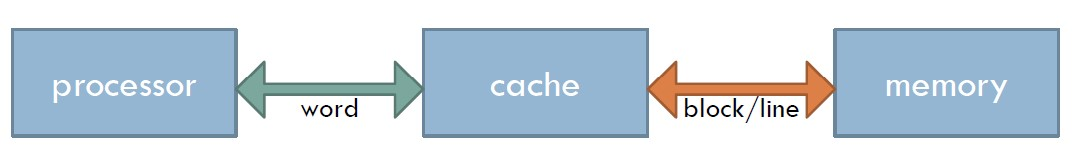
\includegraphics[scale = 1.2]{img/cache.jpg}
        \label{cache}
        \caption{Cache system}
\end{figure}

\begin{itemize}

    \item the data needed by the processor is first fetched into the cache (cache hit or miss), then all subsequent accesses to data items residing in the cache are serviced by the cache. The \textbf{cache hit ratio} is defined as the fraction of memory references that are resolved by the cache memory;
    
    \item performance improves in presence of \textit{high locality}:

    \begin{itemize}
    
        \item \textit{temporal locality}: a data item is re-used after a short amount of time;

        \item \textit{spatial locality}: data with close memory addresses is used within a short amount of time.
        
    \end{itemize}

    \item data transport between cache and main memory is done by the transfer of blocks comprising several words, whereas the processor accesses single words in the cache.
    
    
\end{itemize}

\underline{Example 2 (Memory latency with cache)}: let's consider a processor operating at 1 GHz (1 ns clock) connected to a DRAM with a latency of 100 ns and suppose that we have a cache of 32KB, with a latency of 1 ns per word, and we consider the problem of multiplying two matrices $A$ and $B$ of size 32*32 (we suppose that $A$, $B$ and $A * B$ fit in the cache). Then, the time needed to load $A$ and $B$ into the cache is $32*32*2* 100 ns = 205 \mu s$. Then, multiplying two matrices of size n*n takes $2n^3$ multiply-adds, in our case $2*32^3 = 66K$ multiply-adds, which implies $66 \mu s$. Finally, the total time is $205 + 66 = 271 \mu s$, so the throughput is $\frac{66K * 2}{271} = 488$ MFLOPS (> $10$ MFLOPS of the Example 1) (still < $2$ GFLOPS, which represents the peak processor rating). Moreover, we underline the fact that the locality is exploited by observing that the computational complexity of these operations is $n^3$, but here we are computing using $n^2$ memory locations!


\underline{Example 3 (Bandwidth with cache)}: let's consider the previous example. If the \textit{cache block} has a width of \textit{one single word}, then it takes $32*32*2*100 ns = 205 \mu s$ to load the two matrices in cache. However, if the width is of \textit{four words}, then the overhead is $32*32*2/4*100 ns = 51 \mu s$, with a total time (load into cache + computation) of $51 + 66 = 117 \mu s$. In this case, the throughput is $\frac{66K * 2}{117} = 1282$ MFLOPS (> 488 MFLOPS of Example 2) (> 10 MFLOPS of Example 1) (still < 2 GFLOPS of the peak processor rating).

Along with cache coherence problem, another important issue for the cache is the \textbf{cache-to-memory coherence}, i.e. the problem consisting on when to write to the memory data that have been modified in the cache. There exist two possible alternatives:

\begin{itemize}

    \item \textbf{write-through policy}, i.e. data is immediately written to memory, so a downside is that the write operation is delayed, while the pro is that the memory is always consistent with the content of the cache;

    \item \textbf{write-back policy}, i.e. memory is updated upon eviction. In this case the two major downsides are that the content of the memory may differ from the content of the cache (inconsistency) and that the processor may not need anymore the data that is currently in the cache. An example of inconsistency is represented in the following picture: the processors see different values of $u$ after the event 3.

    \begin{figure}[h!]
		\centering
		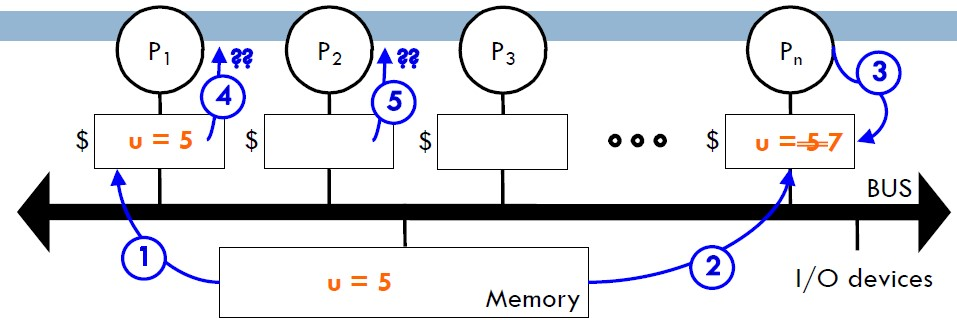
\includegraphics[scale = 0.8]{img/inconsistency.jpg}
        \label{inconsistency}
        \caption{Inconsistency problem}
    \end{figure}
    
    On the other hand, this policy results in having less writing operations;

    \item \textbf{snooping protocols}, most of which assumes that local caches of the processors use a write-through policy and that all memory accesses are performed via the central bus. In this way, each cache controller can observe all write accesses to perform updates or invalidations
    
\end{itemize}

Finally, one last example of important issue concerning cache is the \textbf{false sharing}, which happens when two \textit{unrelated variables}, i.e. variables that are logically private to distinct threads, are allocated in the same block and do not conflict. In this case, from the point of view of the data block the accesses are considered conflicts, even if the two processors access disjoint words of the same block, thus the cache updates are not necessary! In this sense, it is usually a good practice to put on the same block \textit{related variables}.

\subsection{Models}
So far we've seen that the cache has a significant impact on the performance of modern applications, so now we focus both on the cache models and on some algorithms that exploit the cache use, in particular \textit{matrix multiplication} and \textit{sorting}.

\subsubsection{External-Memory Model}
Before analyzing the \textit{cache-oblivious model}, we first review the standard model of a two-level memory hierarchy with block transfers. This model is known as \textbf{external-memory model}, and it defines the computer as having two levels, as represented in Picture \ref{external_memory_model}:

\begin{itemize}
    \item the \textit{cache} which is near to the CPU, cheap to access but limited in space;
    \item the \textit{disk} which is distant from the CPU, expensive to access but nearly limitless in space.
\end{itemize}


\begin{figure}[h!]
		\centering
		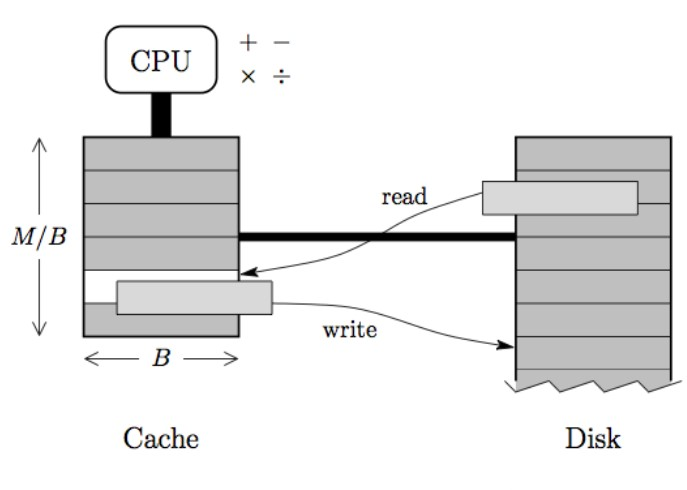
\includegraphics[scale = 1.2]{img/model.jpg}
        \label{external_memory_model}
        \caption{External-Memory model}
\end{figure}

The central aspect of this model is that transfers between \textit{cache} and \textit{disk} involve \textit{blocks} of data: as we can see, each block has size $B$, while the \textit{cache} has size $M \geq B^2$ and contains $M/B$ entries. The main properties of this model are:

\begin{itemize}

    \item it provides a simple description of the relationship between CPU, \textit{cache} and \textit{disk};

    \item the complexity of the algorithms we will consider will be based on the number of \textit{disk} accesses;

    \item the algorithms will be optimized for specific values of $M$ and $B$;

    \item we assume that the cache is working in the best possible way, i.e. it always makes the best possible choices.
    
\end{itemize}

\subsubsection{Cache-Oblivious Model}
The other important cache model is the \textbf{cache-oblivious model}, and its basic idea is to design external-memory algorithms without knowing $B$ and $M$. But this simple idea has several surprisingly powerful \textbf{consequences}:

\begin{itemize}
    \item If a cache-oblivious algorithm performs well between two levels of the memory hierarchy (nominally called \textit{cache} and \textit{disk}), then it must automatically work well between any two adjacent levels of the memory hierarchy;
    \item If the number of memory transfers is optimal up to a constant factor between any two adjacent memory levels, then any weighted combination of these counts (with weights corresponding to the relative speeds of the memory levels) is also within a constant factor of optimal;
    \item The cache-oblivious model does not require to tune the cache parameters, an operation which make the code portability difficult: using this model, an algorithm should work well on all machines without modification.
\end{itemize}

In contrast to the external-memory model, algorithms in the cache-oblivious models \textbf{cannot explicitly manage the cache}, and this is necessary since both $M$ and $B$ are not known. Moreover, this model is based on several \textbf{assumptions}:

\begin{enumerate}
    \item the \textit{ideal cache model} assumes that the \textit{page replacement} operation is \textit{optimal}: in particular, it specifies that the page replacement strategy knows the future and always evicts the page that will be accessed farthest in the future. Real-world caches do not know the future, and employ more realistic page replacement strategies such as evicting the least-recently-used block (\textit{LRU}) or evicting the oldest block (\textit{FIFO});
    \item \textit{Full associativity}, i.e. we assume that any block can be stored anywhere in the cache, in contrast with real-world caches that are characterized by \textit{limited associativity};
    \item \textit{Tall-cache assumption}: the cache is assumed to be tall, i.e. $M = \Omega(B^2)$ (usually a weaker condition is sufficient $M = \Omega(B^{1 + \gamma})$, for any constant $\gamma > 0$). This property is particularly important in some of the more sophisticated cache-oblivious algorithms and data structures, where it ensures that the cache provides a polynomially large “buffer” for guessing the block size slightly wrong. It is also commonly assumed in external-memory algorithms.
\end{enumerate}

While on the one hand these assumptions are really strong, the following theorems make the model described above more feasible to be applied in order to deal with real-world problems, with the running time that degrades only by a constant factor:

\begin{itemize}
    \item \textbf{Lemma 1}: if an algorithm makes $T$ memory transfers on a cache of size $M/2$ with optimal replacement, then it makes at most $2T$ memory transfers on a cache of size $M$ with LRU or FIFO replacement. This means that LRU and FIFO replacement do just as well as optimal replacement up to a constant factor of memory transfers and up a constant factor wastage of the cache;
    \item \textbf{Lemma 2}: for some constant $\alpha > 0$, an LRU cache of size $\alpha M$ and block size $B$ can be simulated in $M$ space such that an access to a block takes $O(1)$ expected time. This result can be reached by using 2-universal has functions and by knowing both $B$ and $M$.
\end{itemize}

By this two theorems we cal conclude that a cache-oblivious model can be translated into a FIFO/LRU cache with 1-associativity paying only constant factors.

\subsection{Algorithms}
We now analyze some important techniques for designing \textbf{cache-oblivious algorithms}.

\subsubsection{Scanning}
The first problem we address is the problem of \textit{scanning}, in which our goal is to traverse all the elements of a set. On a flat memory hierarchy (uniform-cost RAM), such a procedure requires $\Theta(N)$ time for $N$ elements. In the external-memory model, if we store the elements in $\lceil N/B \rceil$ blocks of size $B$, then the number of blocks transfers is $\lceil N/B \rceil$.

To achieve a similar bound in the cache-oblivious model, we can lay out the elements of the set in a contiguous segment of memory, in any order, and implement the $N$-element traversal by scanning the elements one-by-one in the order they are stored: this layout and traversal algorithm do not require knowledge of $B$ (or $M$), and it is represented in Picture \ref{scanning}.

\begin{figure}[h!]
		\centering
		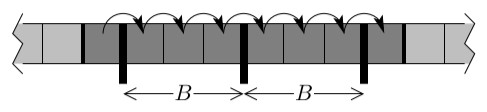
\includegraphics[scale = 1.2]{img/scanning.jpg}
        \label{scanning}
        \caption{Scanning problem in cache-oblivious model}
\end{figure}

The overall complexity using the cache-oblivious model is then $O(\lceil N/B \rceil) + 1$: as we can see, the cache-oblivious bound is an additive 1 away from the external-memory bound, and this is ideal, because normally our goal is to match bounds within multiplicative constant factors.

\subsubsection{Divide and Conquer}
After scanning, the first major technique for designing cache-oblivious algorithms is \textit{divide and conquer}, which often leads to algorithms whose memory-transfers count is optimal within a constant factor. 

The basic idea of this approach is that it \textbf{repeatedly refines the problem size}, until it will eventually \textbf{fit in the cache} (i.e. the size of the problem will be at most $M$) and, later, in a \textbf{single block} (i.e. the size will be at most $B$). The most important \textbf{property} of this approach is that if the number of leaves in the recursion tree is polynomially larger than the divide/merge cost, then the corresponding algorithm will use a number of memory transfers which is optimal within a constant factor.

We will now focus on a specific example of this approach, the \textit{matrix multiplication} problem.

\textbf{Matrix multiplication} \\
The problem of matrix multiplication consists of computing $C = A \cdot B$, where $A$ and $B$ being $N*N$ matrices. The first issue when considering this problem relies on how to store the matrices, and the two possibilities are (Picture \ref{row_column_major}):

\begin{itemize}

    \item \textit{row-major order}:in this case the elements of the matrix are stored by rows, so it is the preferable organization to store matrix $A$;

    \item \textit{column-major order}: in this case the elements of the matrix are stores by columns, so it is preferable organization to store matrix $B$.
    
\end{itemize}

\begin{figure}[h!]
		\centering
		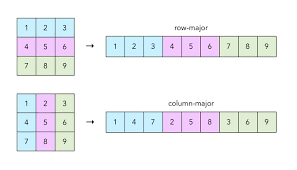
\includegraphics[scale = 0.9]{img/row_column_major.png}
        \label{row_column_major}
        \caption{Row-major order and column-major order representation}
\end{figure}

We can now take into considerations some algorithms to solve this problem.

\colorbox{yellow}{\underline{Algorithm 1}} (naive): this is the simplest algorithm, in which each element $C_{ij}$ is computed by scanning the $i$-th row of $A$ and the $j$-th column of $B$, where $A$ is stored in row-major order and $B$ is stored in column-major order. In this case, the \textbf{number of memory transfers} is given by:

$$
O(N^3/B + N^2)
$$

, since each element of $C$ involves a linear scanning of the row of $A$ and the column of $B$, i.e. $O(N/B + 1)$, and there are $N^2$ elements in $C$. A possible approach to reduce the cost of this algorithm consists of storing the row $i$ of $A$ in cache memory (if $M > N$), or to keep the matrix $A$ in cache (if $M > N^2$).

\colorbox{yellow}{\underline{Algorithm 2}} (external-memory model): this algorithms is based on the idea of multiplying the sub-matrices of $A$, $B$ and $C$, and the \textbf{optimal number of transfers} is $O(N^2/B + N^3/(B * \sqrt{M}))$

An important issue about this algorithm is the choice of the block size, and the optimal choice is to choose a block size $s$ such that $3*s^2 = M$, i.e. such that the cache can contain a block from $A$ and $B$, and that can store the result block of $C$.  

\colorbox{yellow}{\underline{Algorithm 3}} (cache oblivious): this algorithm exploits the \textit{divide-and-conquer} approach by recursively dividing the original matrix into sub-matrices until they fit into the cache, as represented in Picture \ref{mm_cache_oblivious}.

\begin{figure}[h!]
		\centering
		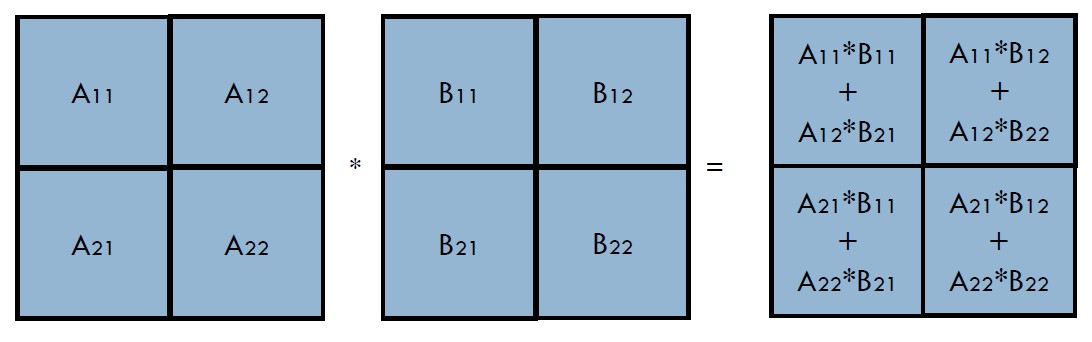
\includegraphics[scale = 0.9]{img/iimproved_algo.jpg}
        \label{mm_cache_oblivious}
        \caption{Divide-and-conquer approach for the matrix multiplication problem}
\end{figure}

Since we do not know in advance when a sub-matrix will fit into the cache, we need a recursive data layout such that however we recursively split the matrix, at some point all the data will be in (almost) consecutive memory locations that can be easily loaded in cache. An example of this organization is the \textit{Z-order representation}. 


The overall \textbf{number of transfers} of this algorithm is given by:

$$
O(N^2/B + N^3/(B \sqrt{M}))
$$

, so it has the same complexity of the external-memory model case.

This particular number of transfers is computed by solving the following recurrence:

$$
T(n) = 8T(N/2) + O(1 + N^2/B)
$$

, where:

\begin{itemize}
    \item $8T(N/2)$ represents the number of transfers of each of the eight multiplication subproblems;
    \item $O(1 + N^2/B)$ represents the number of transfers for each of the four addition subproblems
\end{itemize}


\subsubsection{Sorting} 
We now focus on the sorting problem.

\colorbox{yellow}{\underline{Merge-Sort}} (external-memory model): this algorithm works by recursively splitting the input vector into smaller sub-vectors (\textit{split phase}), by sorting them and by merging them together into the result sorted vector (\textit{merge phase}). We can easily notice that the main operation of the algorithm is represented by the merging phase. 

The best way of implementing this algorithm using an external-memory model is by using the $(M/B)$-way mergesort. In this case, during the merge each memory block maintains the first $B$ elements of each list, and when a block empties, the next block from that list is loaded. It can be shown this algorithm results in the following number of block transfers:

$$
\Theta(N/B \log_{M/B}(N/B))
$$

This number is computed by taking into account these informations:

\begin{itemize}
    \item the recursion tree has $\Theta(N/B)$ leaves;
    \item the leaf cost is $\Theta(N/B)$;
    \item the number of levels in the recursion tree is $\log_{M/B}N$
\end{itemize}

\colorbox{yellow}{\underline{Merge-Sort}} (cache oblivious): the goal of this algorithm is to run the merge phase, the most expensive one, in cache, for any value of $M$ and $B$. In particular, the provided solution consists of implementing a 2-way mergesort, whose complexity is:

$$
\Theta(N/B \log_2(N/M))
$$

Our next goal is then to find a method in order to improve this naive algorithm, in particular by rising the base of the logarithm in order to reach $M/B$. We will reach this goal by using the \textbf{k-funnel} and the \textbf{funnel-sort algorithm}.

\colorbox{yellow}{\underline{Funnelsort}} (cache oblivious): the core of this algorithm is characterized by the \textbf{k-funnel}, which is represented in Picture \ref{funnel}.

\begin{figure}[h!]
		\centering
		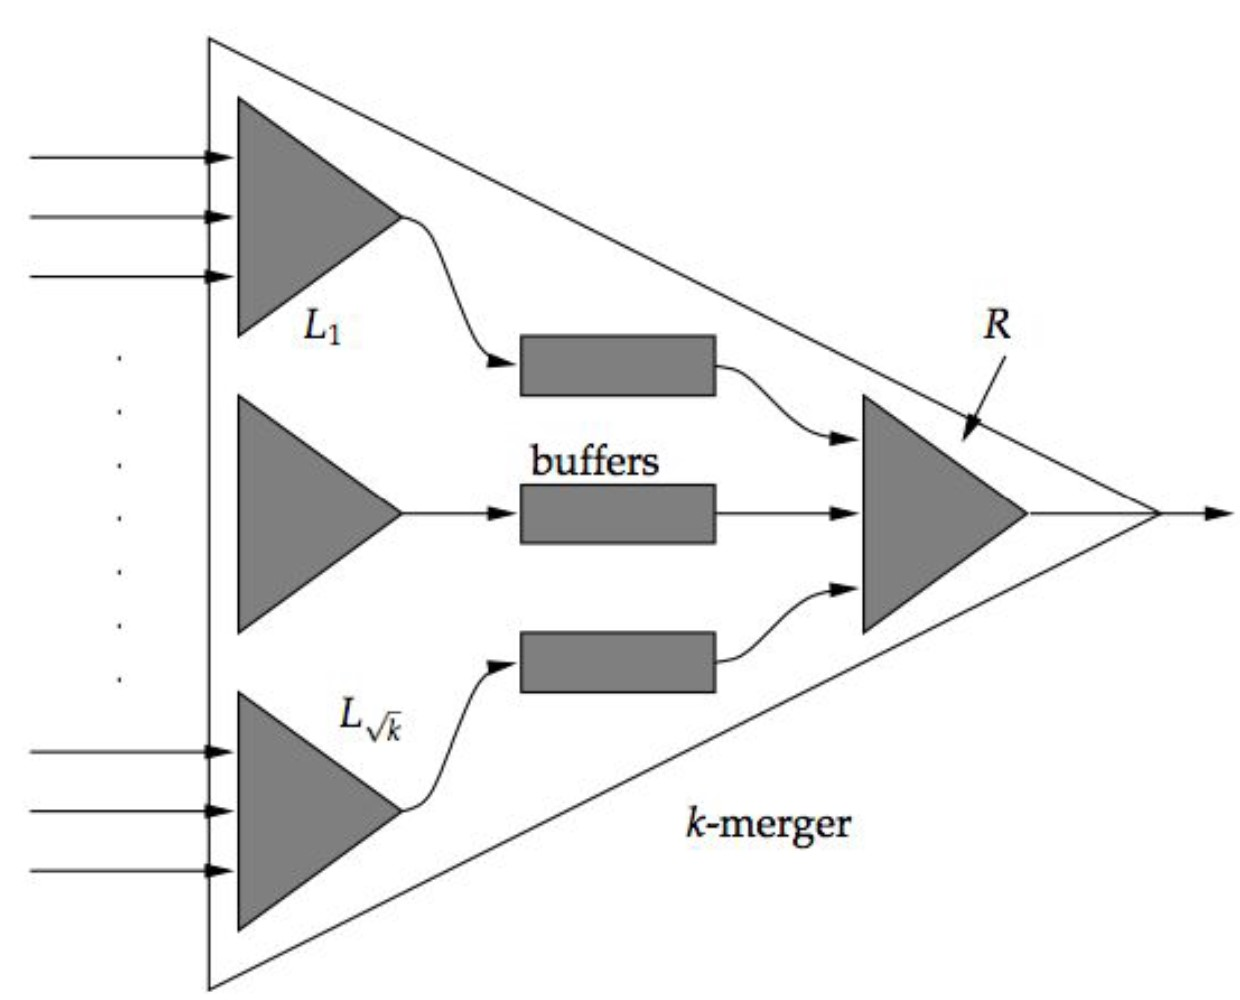
\includegraphics[scale = 0.5]{img/funnel.jpg}
        \label{funnel}
        \caption{k-funnel}
\end{figure}

A \textit{k-funnel} is a merger that merges $k$ sorted lists with total size $k^3 = N$ in a space $k^2$ (note that the cache locality is given by the $k^2 < k^3$ mismatch). More specifically, the \textit{k-funnel} receives in input $k$ sorted lists, that are partitioned into $\sqrt{k}$ groups of size $\sqrt{k}$: each group feeds a $\sqrt{k}$-funnel $L_i$. The output of each $L_i$ is stored in a buffer (FIFO) of size $2k^{3/2} = 2\sqrt{N}$: finally, the $\sqrt{k}$ buffers feed the $\sqrt{k}$-funnel $R$ whose output is the output of the \textit{k-funnel}. An important property of this merger is that if $R$ has buffer $i$ with less than $k^{3/2}$, it recursively invoke $L_i$.

The sizes of the \textit{k-funnel} are the following:

\begin{itemize}
    \item the size of each $L_i$ is $\sqrt{k} * \sqrt{k} = k$;
    \item $R$ has size $k$ as well;
    \item buffers has size $2 * k^{3/2}$
\end{itemize}

, so the total size of the merger is given by $(\sqrt{k} + 1)$ (number of funnels + $R$) + $\sqrt{k} * 2 * k^{3/2}$, which leads to $\Theta(k^2)$.
The \textit{funnelsort} algorithm is the first application of the tall-cache assumption: for simplicity, we assume that $M = \Omega(B^2)$, but the same result can be obtained when $M = \Omega(B^{1 + \gamma})$. Clearly, the crucial issue of this algorithm relies on the choice of the value of $k$: the larger the $k$, the faster the algorithm; however, $k$-funnel is fast only if it is fed at least $K^3$ elements. Thus, $k = N^{1/3}$ is chosen. The algorithm proceeds as follows:

\begin{enumerate}
    \item Split the array into $k = N^{1/3}$ contiguous segments, each of size $N/k = N^{2/3}$;
    \item Recursively sort each segment;
    \item Apply the $k$-funnel to merge the sorted segments.
\end{enumerate}

It can be proven that the \textbf{number of transfers} using the funnelsort algorithm is:

$$
\O(N/B \log_{M/B}(N/B))
$$

, i.e. it is the same as the mergesort using the external-memory model.

\underline{Example}: suppose that $N = 4,096 = 2^{12}$, then the operations of the funnelsort algorithm are:

\begin{enumerate}
    \item Split the array into $k = N^{1/3} = 2^4 = 16$ blocks, each of size $N/k = 2^8 = 256$;
    \item Sort each block independently;
    \item Merge the blocks with a $2^4 = 16$-funnel.
\end{enumerate}

Picture \ref{funnel1} represents the structure of the funnels, while Picture \ref{funnel2} shows the size of each component: note that each buffer has size $2 * k^{3/2} = 2 * 2^6 = 2^7 = 128$, and we recall that if $R$ has buffer $i$ with less than $k^{3/2} = 64$, it recursively invoke $L_i$.

\begin{figure}[h!]
		\centering
		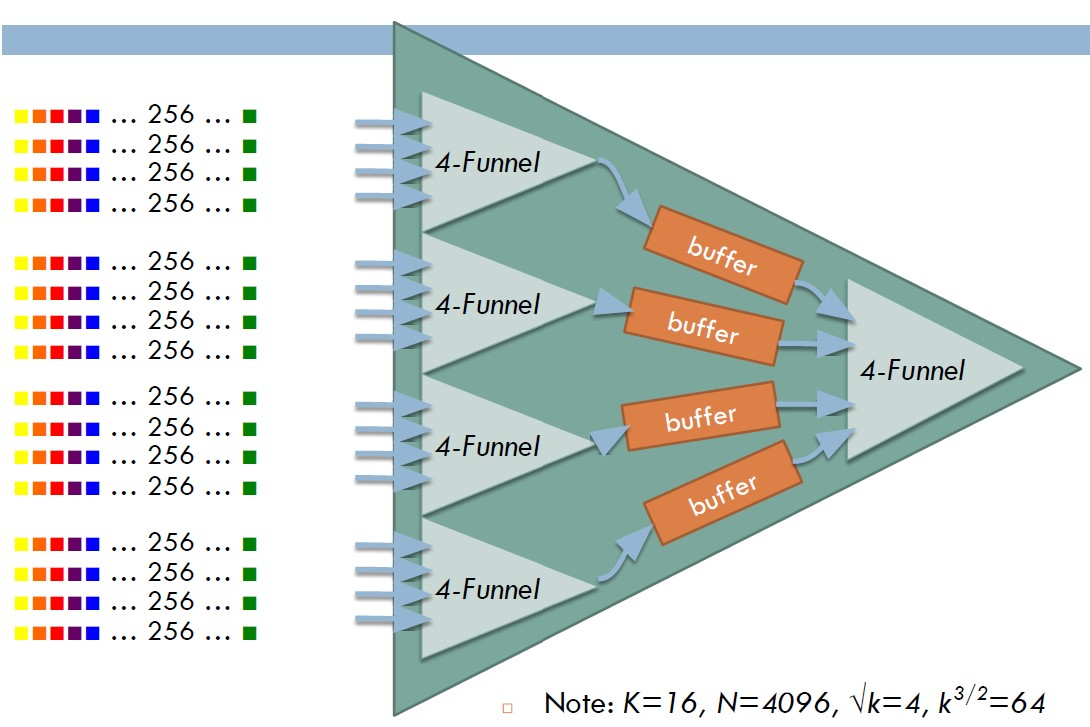
\includegraphics[scale = 0.7]{img/example_funnelsort_1.jpg}
        \label{funnel1}
        \caption{Example of 16-funnel: each buffer has size 128, while R has the same size of the funnel, i.e. 16}
\end{figure}

\begin{figure}[h!]
		\centering
		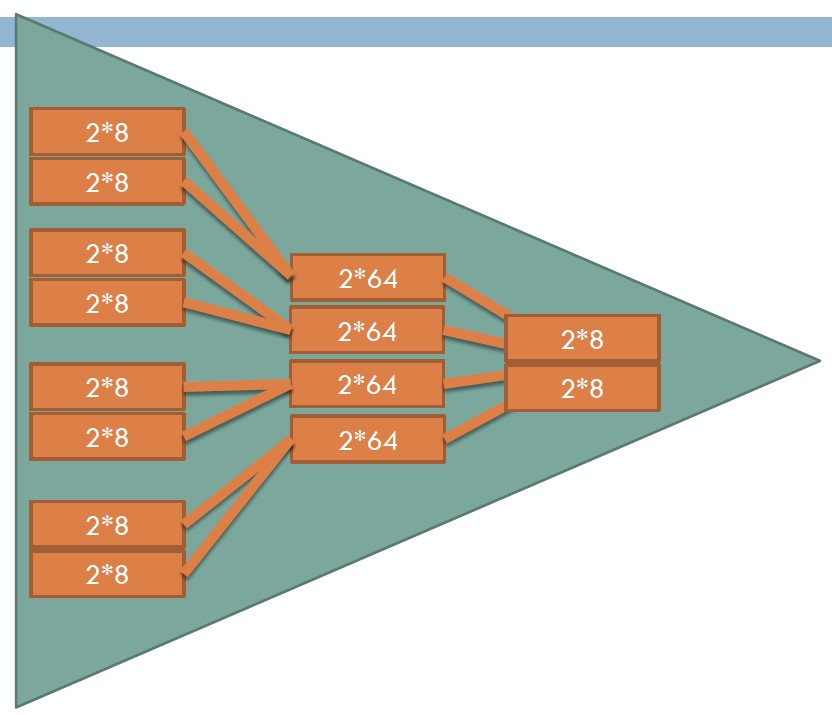
\includegraphics[scale = 0.7]{img/example_funnelsort_2.jpg}
        \label{funnel2}
        \caption{Sizes of the 16-funnel}
\end{figure}

Finally, another important issue about funnelsort is how to efficiently store a k-funnel. One possible solution could be to use a recursive layout, as represented in Picture \ref{funnel_recursive}.

\begin{figure}[h!]
		\centering
		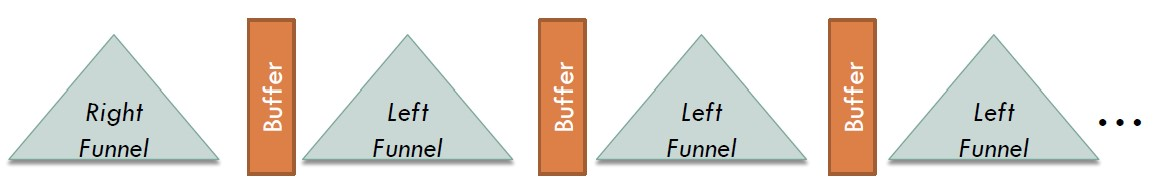
\includegraphics[scale = 0.8]{img/recursive_layout_funnels.jpg}
        \label{funnel_recursive}
        \caption{Recursive layout for a k-funnel}
\end{figure}

However, another possible approach could be to use the so called \textbf{lazy k-funnel}, which is represented as a binary tree of buffers (Picture \ref{lazy_kfunnel}), characterized by the following sizes:

\begin{figure}[h!]
		\centering
		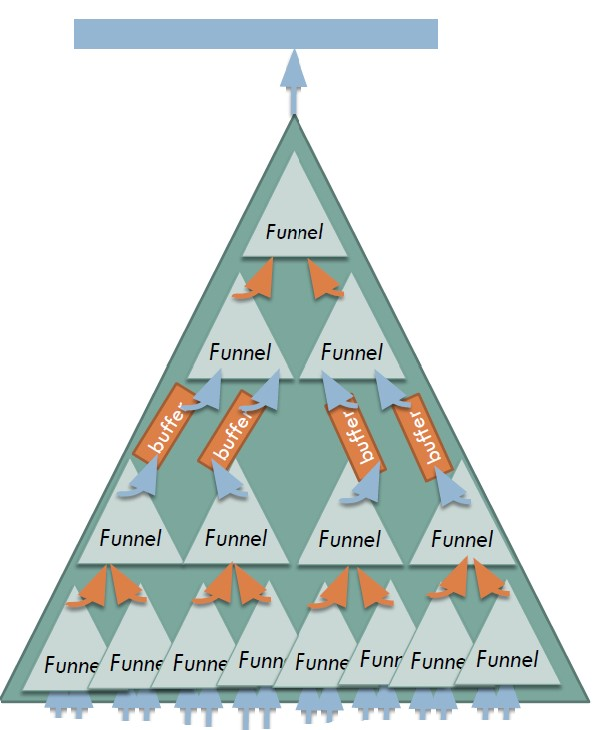
\includegraphics[scale = 0.8]{img/lazy_k_funnel.jpg}
        \label{lazy_kfunnel}
        \caption{Lazy k-funnel}
\end{figure}

\begin{itemize}
    \item the middle layer contains $2 ^ {\lceil \log(k)/2 \rceil}$ buffers, i.e. about $\sqrt{k}$ (in the picture, $k = 16$, so 4 buffers);
    \item each buffer has size $\lceil k^{3/2} \rceil$ (in the picture, the size is 64);
    \item the final buffer, containing the sorted elements, has size $k^3 = N$ (in the picture, $N = 2^{12}$).
\end{itemize}

One peculiarity of this lazy k-funnel is the FILL procedure, through which the buffers are filled, and it is defined as:

\begin{enumerate}
    \item While the buffer is not full:
    \begin{enumerate}
        \item If the left child is empty, then fill it;
        \item If the right child is empty, then fill it;
        \item Perform one merge step
    \end{enumerate}
\end{enumerate}

\subsection{Multicore Hierarchies: Key Challenge}
A crucial issue about the theory underlying the ideal cache model is that it falls apart once we introduce \textbf{parallelism}, i.e. good performances for any $M$ ans $B$ on a 2-level hierarchy do not imply good performances at all levels of hierarchy. This is mainly due to the fact that the \textbf{caches are not fully shared}, and for this reason the \textbf{scheduling} of \textbf{parallel threads} has a \textbf{large impact} on cache \textbf{performances}. Finally, the best technique to deal with caches and threads is to share a largely overlapping working set. 

\subsection{Other approaches}
Among other approaches for hiding the memory latency we can distinguish:

\begin{itemize}

    \item \textbf{multi-threading}, which consists in splitting the problem into multiple sub-problems and in running an independent thread for each sub-problem. Note that when a thread is idle on a miss, another thread can execute computational tasks;

    \item \textbf{pre-fetching}, which consists in anticipating load operations, so that data is already available when needed;

    \item \textbf{drawbacks}, which impact both on bandwidth and on cache pollution.
    
\end{itemize}

\section{Threads}\label{ch3}
In general, when we deal with parallel programs, the total CPU time spent by a parallel implementation is larger than a serial one, because parallelism involves an additional overhead caused by:

\begin{itemize}
    \item Synchronization and communication between threads;
    \item Exchange of data between threads;
    \item Load imbalance, i.e. threads that deal with smaller problems remain idle until other threads deal with bigger ones.
\end{itemize}

\subsection{Evaluation metrics}

Moreover, in general, evaluating a parallel algorithm is difficult, since its performances may depend on the architecture, on the network etc.. Some simple measures are:

\begin{itemize}
    \item The \textbf{parallel runtime $T_p(n)$}, where $p$ is the number of parallel units (cores), and $n$ is the problem size;
    \item The \textbf{cost $C_p(n) = pT_p(n)$}, which represents the total amount of work that is performed.
\end{itemize}

A parallel algorithm is said to be \textbf{cost optimal} if 

$$
C_p(n) = p T^*(n)
$$

, where $T^*(n)$ is the runtime of the fastest sequential algorithm for the given problem. In this sense, a parallel algorithm is cost-optimal if its cost has the same asymptotic growth as the fastest serial algorithm (as a function of the input size).

Another important metric for comparing sequential and parallel algorithms is the \textbf{speedup}, which is defined as:

$$
S_p(n) = \frac{T^*(n)}{T_p(n)}
$$

Theoretically, $S \leq p$, but in practice $S < p$, i.e. we have a \textit{sublinear speedup}, mainly due to the overheads we discussed before. Picture \ref{speedup} represents the speedup w.r.t to the number of processors.

\begin{figure}[h!]
		\centering
		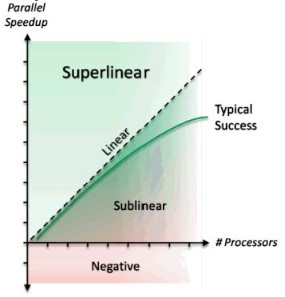
\includegraphics[scale = 1.5]{img/speedup.jpg}
        \label{speedup}
        \caption{Speedup vs number of processors}
\end{figure}

The goal when we implement a parallel algorithm is to measure a \textit{linear speedup}, i.e. $S = p$, and it is even possible to have \textit{superlinear speedup} because of cache sharing.

An alternative measure is \textbf{efficiency}:

$$
E_p(n) = \frac{S(n)}{p} = \frac{T^*(n)}{p T_p(n)}
$$

, and it is a measure of resource usage: it represents the fraction of time the processors are fully used to execute a fraction $1/p$ of the best sequential algorithm. We have that $E = 1$ for linear speedup.

When we deal with the evaluation of parallel algorithms, we have to consider two very important laws: the Amdahl's law and the Gustafson's law. The \textbf{Amdahl's law} regards speedup and says that the parallel execution time $T_p$ cannot be arbitrarily reduced by increasing $p$, i.e. the number of parallel units. If we suppose that a fraction $f$ of the computation cannot be executed in parallel (for example because of some dependencies), the have that:

$$
S_p(n) = \frac{T_{\text{seq}}}{T_{\text{par}}} = \frac{T_{\text{seq}}}{(f * T_{\text{seq}} + (1-f) * \frac{T_{\text{seq}}}{p})} = \frac{1}{f + \frac{1-f}{p}} \leq \frac{1}{f}
$$

, i.e. the sequential fraction $f$ is an upper bound of the speedup $S_p(n)$.

The \textbf{Gustafson's law} on the other hand regards scalability, and in particular it studies the behaviour of the algorithm when $n \to \infty$. In general, when we have a large amounts of data we would like to use a large number of processors. Suppose that the sequential part $c$ of an algorithm is constant w.r.t. to $n$. Then, let $T(n,p)$ be the execution time of the parallelizable part over $p$ processors: we define the \textbf{scaled speedup} as:

$$z
S_p(n) = \frac{c + T_1(n)}{c + T_p(n)} = \frac{c + T_1(n)}{c + \frac{T_1(n)}{p}} = \frac{\frac{c}{T_1(n)} + 1}{\frac{c}{T_1(n)} + \frac{1}{p}}
$$

When $n \to \infty$, we have:

$$
\lim_{n \to \infty} S_p(n) = p
$$

In general, the \textbf{scalability} of a parallel system is its ability to increase the speedup in proportion to the number of processors: scalable algorithms are characterized by a constant efficiency when increasing both the number of processors and the problem size.

\subsection{Shared-memory programming models}
\begin{itemize}
    \item \textbf{Process based models} assume that all data associated with a process is private by default, unless otherwise specified. Moreover, distinct page tables exist for each process in order to map the virtual addresses to distinct physical memory addresses. In this case, processes are units of resource ownership, i.e. they have their own program counter, heap memory etc.. Note that process can include more threads;
    \item \textbf{Thread based models} assume that all memory is global, i.e. the threads share the same address space (same page table), and there's at least one thread per process. Note that in this case the communication between the threads is far more easy than in the process based model;
    \item \textbf{Directive based models}: in this case the concurrency is specified in terms of high-level compiler directives, resulting in a sort of "annotated" source code. An example is given by the OpenMP library.
\end{itemize}

\subsection{pthreads}
In general, each thread has a separate execution flow, and it is the owner of a private program counter, stack memory, stack pointer etc.. , and they're also known as \textit{lightweight processes}. In this course we analyze the \textbf{pthreads} library (POSIX threads).

An example of the usage of the threads can be viewed in the matrix multiplication problem, as represented in Picture \ref{mm_threads}.

\begin{figure}[h!]
		\centering
		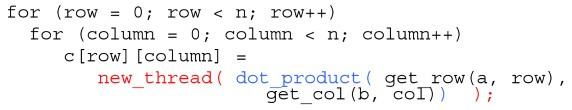
\includegraphics[scale = 1.5]{img/mm_threads.jpg}
        \label{mm_threads}
        \caption{Matrix multiplication with threads}
\end{figure}

In this case, we can consider a thread as the parallel asynchronous execution of a function with its parameters. In the \textit{pthreads} library, all the threads in a process are peers, and there's no explicit parent-child model, with the exception of the "main thread" that holds the process information. The main advantages over the processes are that threads can read/write to shared variables for communication, and that the context-switch operation is faster. The life cycle of a thread is represented in Picture \ref{threads}.

\begin{figure}[h!]
		\centering
		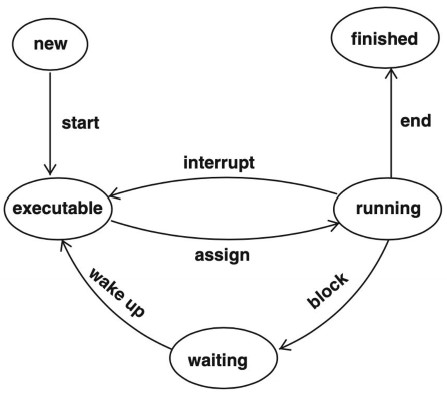
\includegraphics[scale = 1.5]{img/threads.jpg}
        \label{threads}
        \caption{Life cycle of a thread}
\end{figure}

An example of code that exploits the threads is shown in Picture \ref{pthreads example}.

\begin{figure}[h!]
		\centering
		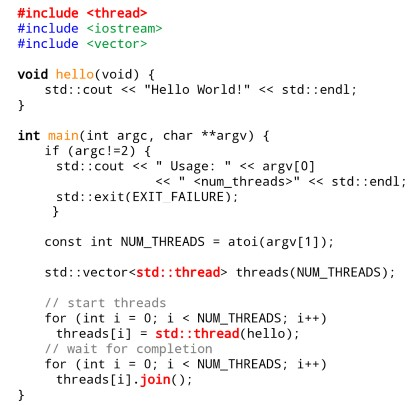
\includegraphics[scale = 1.7]{img/pthreads example.jpg}
        \label{pthreads example}
        \caption{Example of usage of threads}
\end{figure}

\begin{itemize}
    \item A vector of \textit{std::thread} objects is created. Notice that each thread object must be associated to a single actual thread;
    \item In the first for loop, each actual thread is created by passing the function \textit{hello}, which has no parameters;
    \item The second for loop is used to wait each thread to complete the execution, and this is done by the \textit{join} function.
\end{itemize}

In general, the class \textit{std::thread} is used to represent individual threads of execution: a thread is joinable, and it has a unique thread id. As we said before, a non-initialized thread does not represent a thread. The typical contructor for a thread is \textit{thread (function, arg1, arg2, .., argn)}, where the new thread of execution calls \textit{function} passing \textit{arg1, arg2, .., argn} as arguments. As we said before, no two \textit{std::threads} objects may represent the same thread of execution!

Other important functions are:

\begin{itemize}
    \item \textit{void join()}, which returns when the thread execution has completed, and after a call to this function, the thread object becomes non-joinable;
    \item \textit{void detach()}, which separates the thread of execution from the thread object, while the underlying thread executes independently;
    \item \textit{hardware\_concurrency()} returns the number of hardware thread contexts;
    \item \textit{void this\_thread::yield()}, which suggests the OS to re-schedule so as to allow other threads to be executed;
    \item \textit{void this\_thread::sleep\_for(duration)}, which stops the execution of the thread for duration, and the actual restart depends on OS scheduling decisions;
    \item \textit{void this\_thread\_sleep\_until(time\_point)}, which stops the execution until time\_point is reached. As before, the actual restart depends on OS scheduling decisions.
\end{itemize}

\colorbox{yellow}{\underline{Example}} (PI computation): the formula for deriving the value of $\pi$ can be approximated as:

$$
\pi = \frac{1}{n} \sum \limits_{i = 1}^n \frac{4}{1 + (\frac{i - 0.5}{n})^2}
$$

, the larger the $n$, the better the precision in the calculation of $\pi$. The idea to parallelize this computation is to split the work among the threads, in particular by assigning each thread a term of the summation, and then sum them up. Picture \ref{pi_function} shows the function that is called for each thread, while the others show the main.

\begin{figure}[h!]
		\centering
		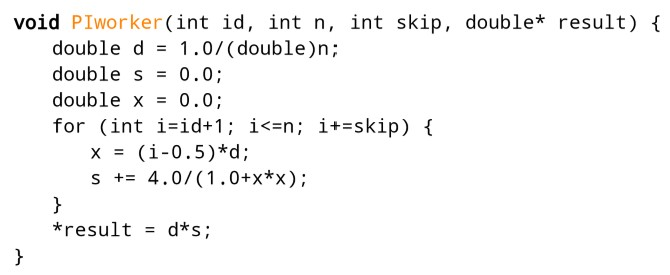
\includegraphics[scale = 1.4]{img/pi_thread.jpg}
        \label{pi_function}
        \caption{Function than computes the $\pi$}
\end{figure}

\begin{figure}[h!]
		\centering
		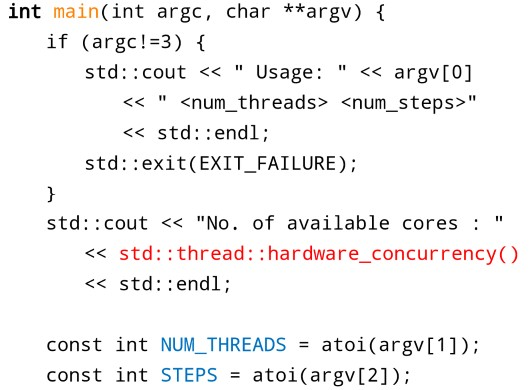
\includegraphics[scale = 0.8]{img/pi_main1.jpg}
        \label{pi_thread}
\end{figure}

\begin{figure}[h!]
		\centering
		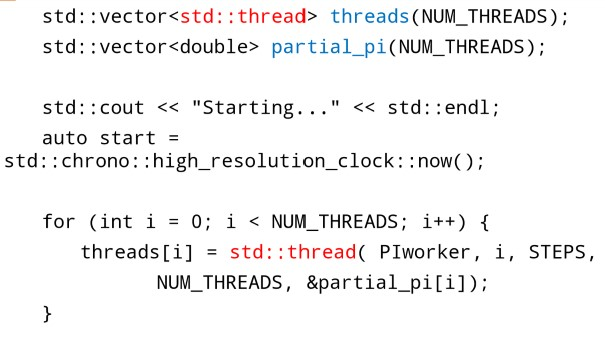
\includegraphics[scale = 0.8]{img/pi_main2.jpg}
        \label{pi_thread}
\end{figure}

\begin{figure}[h!]
		\centering
		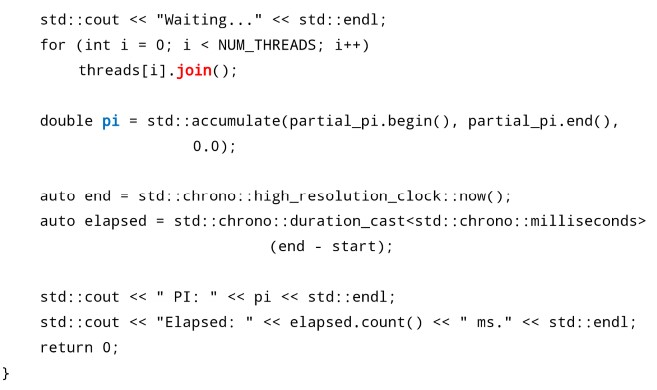
\includegraphics[scale = 0.8]{img/pi_main3.jpg}
        \label{pi_thread}
\end{figure}

As regards the \textit{PIworker} function:

\begin{itemize}
    \item the \textit{int skip} parameter determines the distance between the work of a thread and the work of another thread, since the work of the threads is interleaved;
    \item the result is stored into a variable, so it is not returned.
\end{itemize}

As regards the main:

\begin{itemize}
    \item we read from the terminal the number of threads and the value for the \textit{skip} parameter;
    \item a vector of threads is created: each thread writes in different part of the memory;
    \item a vector of double is created, to store the partial results.
\end{itemize}

\subsection{Mutex}
When multiple threads are manipulating the same data, results can be incoherent: we call \textit{critical section} the portion of code where a race condition occurs, and the idea of the \textit{mutual exclusion} is that at any point of time, only one thread can be in the critical section. In this sense, the \textit{mutex} is an object that prevents other threads with the same protection from executing concurrently and access the same memory locations. The main functions are:

\begin{itemize}
    \item \textit{void lock()}, to get the lock;
    \item \textit{void unlock()}, to release the lock;
    \item \textit{bool try\_lock()}, returns True if the lock was acquired;
    \item \textit{std::recursive\_mutex}, allows a thread to lock the same mutex multiple times;
    \item \textit{std::timed\_mutex}.
\end{itemize}

\colorbox{yellow}{\underline{Example}} (Consumer/Producer): the scheme of the consumer/producer problem is shown in Picture \ref{consumer_producer}. IN particular, the producer puts an item in the queue for 10 times, while the producer gets an item from the queue only it is not empty, again for 10 times. As we can see, the queue represents a critical section, since both the consumer and the producer access to it.

\begin{figure}[h!]
		\centering
		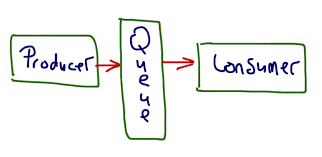
\includegraphics[scale = 0.8]{img/consumer producer.png}
        \label{consumer_producer}
        \caption{Consumer/Producer}
\end{figure}

Picture \ref{main} shows the main function to resolve the Consumer/Producer problem, while Picture \ref{consumer} and \ref{producer} shows the consumer and producer functions.

\begin{figure}[h!]
		\centering
		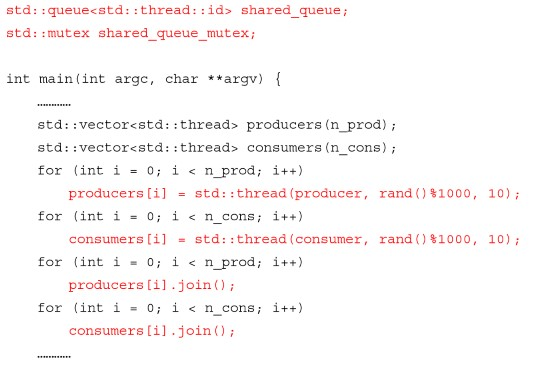
\includegraphics[scale = 1.4]{img/cp_main.jpg}
        \label{main}
\end{figure}

\begin{figure}[h!]
		\centering
		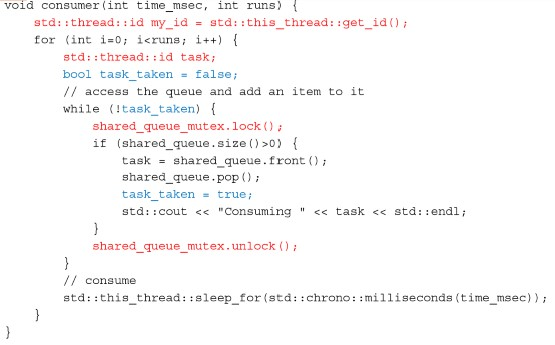
\includegraphics[scale = 1.4]{img/cp_c.jpg}
        \label{consumer}
\end{figure}

\begin{figure}[h!]
		\centering
		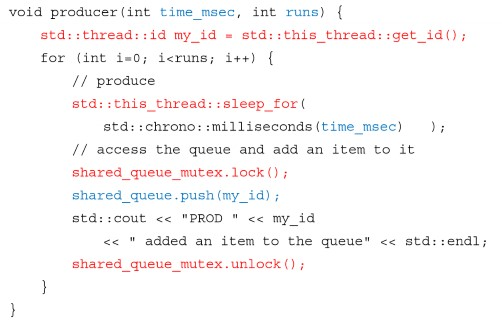
\includegraphics[scale = 1.4]{img/cp_p.jpg}
        \label{producer}
\end{figure}

For what regards the main:

\begin{itemize}
    \item we see that both a queue of thread IDs and a mutex are defined;
    \item a vector of threads is created, both for consumer and for producer: each consumer and each producer executes the respective function, then they're joined.
\end{itemize}

For what regards the producer, we see that before adding an item to the queue, the mutex is locked; then, after the writing, the mutex is unlocked, otherwise a deadlock would result. For what regards the consumer, we see that before reading the content of the queue, the mutex is locked, then if the queue is not empty, the value is read. Finally, the mutex is unlocked.

However, usually the mutexes are not used directly, but through:

\begin{itemize}
    \item \textit{lock\_guard(mutex)}, which allows to acquire a given mutex when created, and to release it when the end of the scope is reached;
    \item \textit{scoped\_lock}, which is similar to the previous one, but the locks are acquired and released on multiple mutexes.
\end{itemize}

, which allows easier handling and error free in case of exceptions or other issues. Moreover, the function \textit{std::call\_once(flag, callable, arg1..)} is used to make sure that a given function is executed only once even if invoked by multiple threads. The arguments are:

\begin{itemize}
    \item \textit{flag}, which should be an instance of \textit{std::once\_flag};
    \item \textit{callable}, which is a callable object, i.e. a function or anything supporting the () operator;
    \item \textit{arg1,..} are the arguments passed to the \textit{callable}.
\end{itemize}

Picture \ref{revised_producer} and \ref{revised_consumer} shows the revised implementation of the consumer and producer functions adopting the functions defined above.

\begin{figure}[h!]
		\centering
		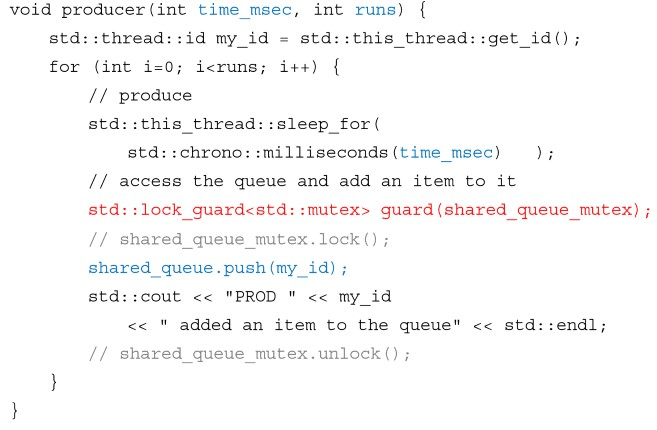
\includegraphics[scale = 1.4]{img/cp_revised_p.jpg}
        \label{revised_producer}
\end{figure}

\begin{figure}[h!]
		\centering
		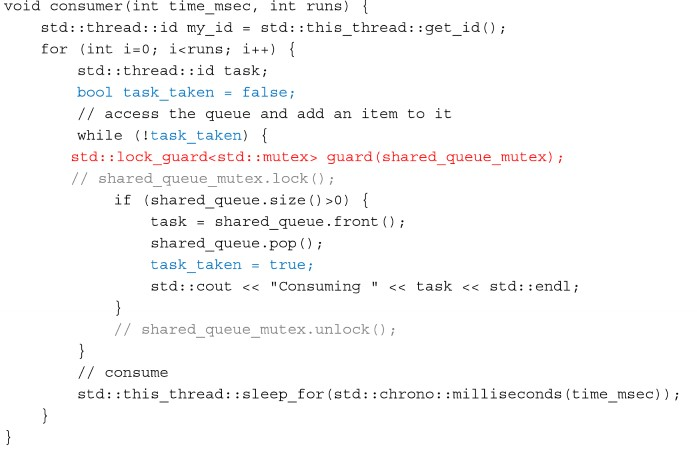
\includegraphics[scale = 1.4]{img/cp_revised_c.jpg}
        \label{revised_consumer}
\end{figure}

As we can see, the producer initialize a \textit{lock\_guard} passing the mutex as a parameter, and in this way the mutex is automatically locked and unlocked, so the \textit{lock()} and \textit{unlock()} functions are not needed anymore. On the other hand, the consumer does the same thing, so again the \textit{lock()} and \textit{unlock()} functions are not used.

Another useful tool that can be used are the \textbf{condition variables}, which allow a thread to block itself until specified data reaches a predefined state, which is checked by a predicate. In this sense, a condition variable can be thought as a notification system on the status of a variable, and it always has a mutex associated to it. The functioning is the following:

\begin{enumerate}
    \item A thread checks some data: if the data is ok it does some work, otherwise it waits;
    \item At some point the thread is awakened: it must re-check the data, since other threads may have been waiting for the same event and they may have already changed the status of the data.
    \item When a different thread modifies the data and reaches the desired status, it signals all the waiting threads.
\end{enumerate}

Notice that the shared data is accessed in mutual exclusion. If we consider the consumer/producer problem, we have:

\begin{itemize}
    \item the producer acquires a mutex, modifies the data and \textit{notify\_one} or \textit{notify\_all} on the condition variable, to wake up one or all threads on waiting;
    \item the consumer acquires s unique lock and executes the \textit{wait}, \textit{wait\_for} or \textit{wait\_until}. Then, the thread is awakened, it checks the condition and accesses the data.
\end{itemize}

Picture \ref{condition_p} and \ref{condition_c} shows the functions of the consumer and producer using the condition variable.

\begin{figure}[h!]
		\centering
		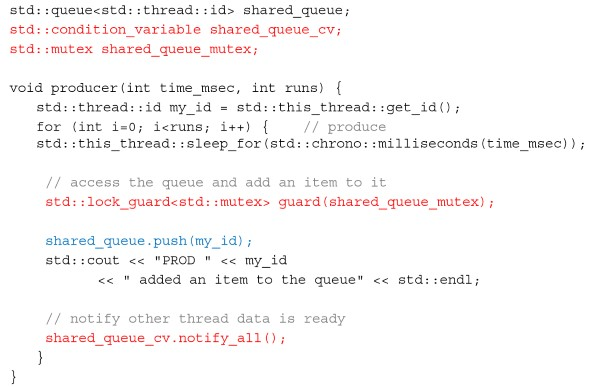
\includegraphics[scale = 1.4]{img/condition_p.jpg}
        \label{condition_p}
\end{figure}

\begin{figure}[h!]
		\centering
		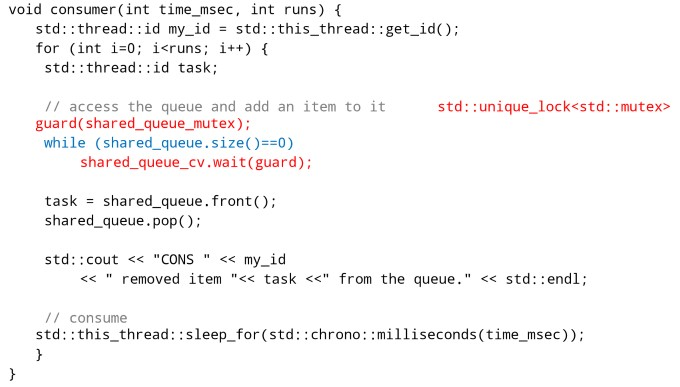
\includegraphics[scale = 1.4]{img/condition_c.jpg}
        \label{condition_c}
\end{figure}

As we can see, the condition variable \textit{shared\_queue\_cv} is created, and the producer notifies all the treads after writing in the queue. On the other hand, the consumer waits until the queue is not empty, and then it consumes the produced data. Notice that the while loop is very useful since many consumers may be waken up, so the loop is used to check whether some other consumer consumed the produced data. Moreover, we notice that the consumer waits on a unique lock.

Finally, other important tools are \textbf{atomic} and \textbf{promise/future}. The \textbf{atomic} creates a new variable whose modification and access does not cause data races. The \textbf{promise/future} tool allows to implement the communication between threads in a convenient way. An example is showed in Picture \ref{future_1} and \ref{future_2}.

\begin{figure}[h!]
		\centering
		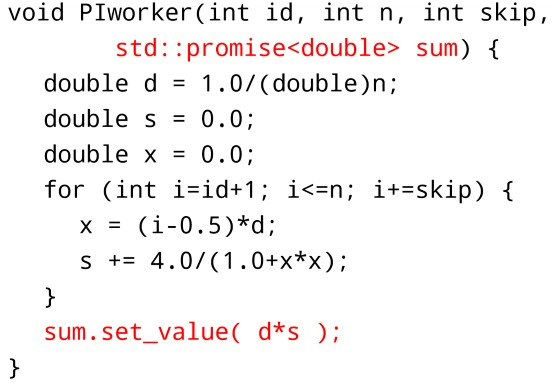
\includegraphics[scale = 1.4]{img/futures_pi.jpg}
        \label{future_1}
\end{figure}

\begin{figure}[h!]
		\centering
		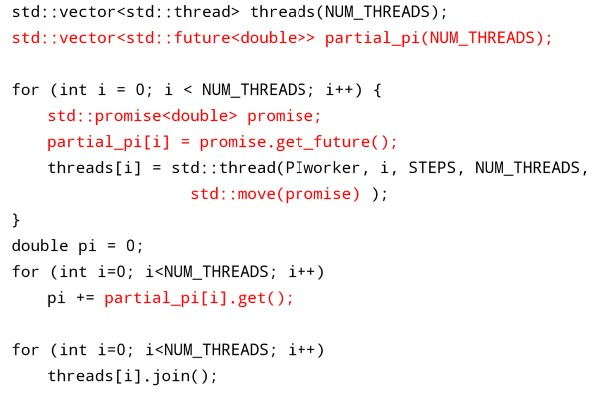
\includegraphics[scale = 1.4]{img/futures_pi_2.jpg}
        \label{future_2}
\end{figure}

Another way to launch a thread is by using the \textit{std::threads(std::launch policy, Function&& f, arg1,..)}, which runs the given function $f$ asynchronously and returns a \textit{std::future} that will eventually hold the result of that function call. The \textit{policy} can be:

\begin{itemize}
    \item \textit{async}, i.e. it creates a new thread that executes $f$ immediately;
    \item \textit{deferred}, i.e. the task is executed on the calling thread the first time its result (future) is requested
\end{itemize}

\subsection{OpenMP}
OpenMP is a very useful library for parallelizing some common patterns, e.g. for-loop, and it works by writing some instructions for the compiler, that automatically parallelizes the operations we indicate. In this sense, it provides the programmer a higher level of abstraction than pthreads, and it supports:

\begin{itemize}
    \item Parallel execution;
    \item Parallel loops;
    \item Critical sections;
    \item etc..
\end{itemize}

The OpenMP \textbf{directives} are based on the \textbf{\#pragma} compiler directives, and they consist of a directive name followed by some clauses, i.e. \textbf{\#pragma omp \textit{directive} [clause list]}. The OpenMP programs execute serially until they encounter the \textit{parallel} directive, which creates a team of threads that execute in parallel the given block. The main thread that encounters the parallel directive becomes the \textit{master} of the team of threads, and it is assigned with the thread id 0 within the group. We notice that despite executing in parallel the portion of code, no information is provided about the first thread that executes, the second etc.., i.e. the execution flow of each thread is not known.

\subsubsection{Basic clauses}
The \textbf{basic clauses} of the OpenMP library are:

\begin{itemize}
    \item \textit{num\_threads (int)}, that specifies the degree of concurrency, i.e. the number of threads that are created;
    \item \textit{if (scalar expression)}, that specifies the conditional parallelization, i.e. whether the parallel construct results in creation of not. If the expression evaluates false, the only one existing thread executes the following instruction block.
\end{itemize}

An example of the usage of this bases clauses is provided in Picture \ref{basis_clauses}.

\begin{figure}[h!]
		\centering
		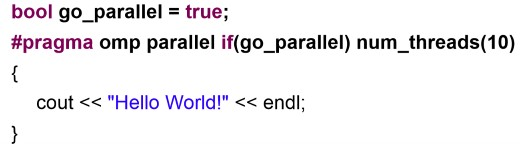
\includegraphics[scale = 1.4]{img/basis clauses.jpg}
        \label{basis_clauses}
\end{figure}

\subsubsection{Variable sharing clauses}
In OpenMP we can specify the level at which the variables of the code are shared among the threads that are created (in the following list, $x$ refers to a variable outside the block which can be accessed by the threads):

\begin{itemize}
    \item \textbf{private(x)}: in this case each thread has his own copy of $x$; $x$ is not initialized, so its initial value is undefined;
    \item \textbf{shared(x)}: in this case every thread accesses the same memory location, so it introduces race condition;
    \item \textbf{firstprivate(x)}: in this case each thread has his own copy of $x$, and $x$ is initialized with the current value of $x$ before the various threads start;
    \item \textbf{default (shared/none)}: affects all the variables not specified in other clauses
\end{itemize}

An example of the functioning of these clauses is provide in Picture \ref{variable_sharing}: as we can see, the number of threads is 10, and the variable $a$ is accessed as private, $b$ and $d$ are shared, while $c$ is firstprivate. In this sense, we see that the value of $a$ and $c$ at the end of the block are 1, since the increments are done in the private copies of the threads, while the values of $b$ and $d$ are 11, since they're incremented by each of the 10 threads.

\begin{figure}[h!]
		\centering
		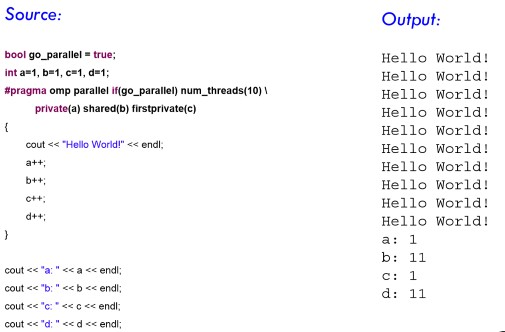
\includegraphics[scale = 1.6]{img/variable sharing clauses.jpg}
        \label{variable_sharing}
\end{figure}

It is important to notice that there's no guarantee that for the \textit{shared} variables the increments are atomic, so the result of the previous code could also be different from 11 in some cases, due to the race condition described above.

\subsubsection{Reduction clause}
The \textbf{reduction clause} specifies how multiple \textbf{local copies} of a variable at different threads are \textbf{combined} into a single copy at the master when threads exit. The clause is defined as \textit{reduction (operator: variable list)}, where:

\begin{itemize}
    \item each variable of the list is accessed as \textit{private} by each thread, and the variable is initialized as the value which is neutral w.r.t. the \textit{operator} (if +, then it is initialized as 0, if * as 1 etc..);
    \item the \textit{operator} can be one of +, *, -, &, |, etc..
\end{itemize}

An example of the functioning of reduction clause is provided in Picture \ref{reduction_clauses}. As we can see, $b$, $c$ and $d$ are shared, so their values are 11, while the value of $a$ is incremented in each thread to 2, then it is reduced using the * operator, so the overall computation is $2*2*..*2 = 2^{10} = 1024$.

\begin{figure}[h!]
		\centering
		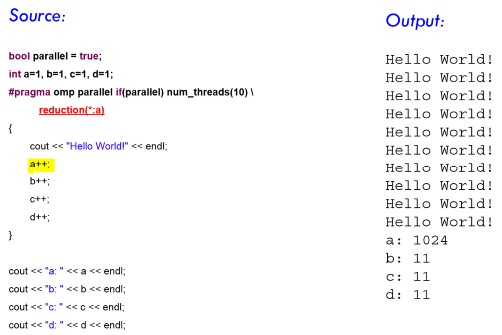
\includegraphics[scale = 1.6]{img/reduction clauses.jpg}
        \label{reduction_clauses}
\end{figure}

\subsubsection{\textit{for} directive}
OpenMP provides a directive \textit{for} to split iterations of the subsequent for loop among available threads: an example is provided in Picture \ref{for_clause}. As we can see, the code computes the sum of the first 10 squared numbers, and the variable \textit{add} is reduces according to the operator +.

\begin{figure}[h!]
		\centering
		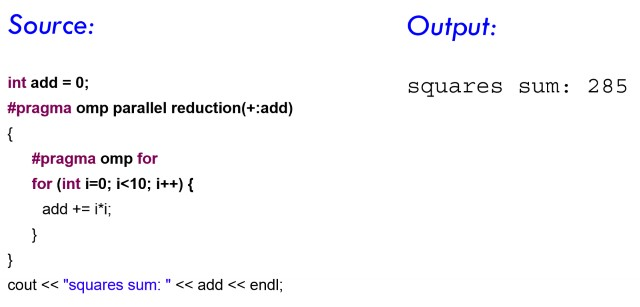
\includegraphics[scale = 1.6]{img/for clause.jpg}
        \label{for_clause}
\end{figure}

An additional clause can be attached to the \textit{for} directive, and it is the \textit{schedule} clause. The \textit{schedule}  is defined as \textit{schedule (policy [, param])}, and it deals with the assignment of iterations to each thread. The policies can be:

\begin{itemize}
    \item \textbf{schedule(static)}: in this case the loop is statically split into chunks and each chunk is statically assigned to a thread. Notice that we still do not know in which order the chunks will be executed;
    \item \textbf{schedule(dynamic)}: in this case the loop is statically split into chunks, and each thread asks for the next chunk to be executed. We do not know how much chunks each thread will execute, but this policy is useful to balance the load;
    \item \textbf{schedule(guided)}: in this case the chunk size decreases exponentially in time. Long tasks are assigned soon to minimize any overhead, while short tasks are assigned at the end to avoid idle threads and to have threads that complete their chunks at the same time;
    \item the \textit{param} specifies the chunk size; if the policy is \textit{guided}, then it specifies the minimum chunk size.
\end{itemize}

Other additional clauses are the \textit{nowait} clause and the \textit{ordered} directive. The \textit{nowait} clause enables the thread that completed the for loop execution to proceed the parallel execution of the rest of the code, while the \textit{ordered} directive forces a piece of code to be executed according to the natural order of the for loop. 

Finally, there are some restrictions in order to apply the \textit{for} directive:

\begin{itemize}
    \item for loops must not have break statements;
    \item loop control variable must be integer, as its initialization expression;
    \item the logical expression must be of $<, \leq, > , \geq$;
    \item the increments/decrements must have integers.
\end{itemize}

\subsubsection{Sections}
OpenMP supports non-iterative parallel task assignment using the \textit{sections} directive: in this case, each section is executed by only one thread (in parallel). There exist some synchronization directives:

\begin{itemize}
    \item \textbf{barrier}: all the threads must wait for each other to reach the barrier;
    \item \textbf{single[nowait]}: the following structures block enclosed is executed by only one thread in the team. Threads in the team that are not executing the single single block have to wait at the end of the block unless \textit{nowait} is specified;
    \item \textbf{master}: only the master thread of the team executes the block enclosed by this directive, the others skip it and continue;
    \item \textbf{atomic}, which ensures atomicity of expressions like $x++, ++x, x--, --x$ etc..;
    \item \textbf{critical[(name)]}, which restricts access to the structured block to only one thread at a time. The optional name argument identifies the critical region: no two threads can enter the critical section with the same name.
\end{itemize}

\subsubsection{Synchronization issues}
OpenMP is able to synchronize shared variable, but the \textbf{compiler} may unpredictably optimize the code, and in general it uses a minimum effort approach on synchronization. The \textit{flush(var list)} directive can be used to synchronize a set of shared variables among the threads in the team.

\subsubsection{OpenMP vs explicit thread management}
\begin{itemize}
    \item Directives layered on top of threads \textbf{facilitate a variety of
    thread-related tasks}, and the programmer is \textbf{rid of the tasks} of initializing attributes objects, setting up arguments to threads, partitioning iteration spaces, etc..;
    \item However, using explicit threading the \textbf{data exchange is more apparent}, and this helps in alleviating some of the overheads from data movement, false sharing, and contention. Explicit threading also provides a \textbf{richer API} in the form of condition waits, locks of different types, and increased flexibility for building composite synchronization operations;
    \item Finally, since explicit threading is used more widely than OpenMP, \textbf{tools and support} for Pthreads programs are \textbf{easier} to find.
\end{itemize}

\colorbox{yellow}{\underline{Example}} ($\pi$ computation): Picture \ref{pi_computation} shows the code for the parallel computation of $\pi$. We recall that the formula is 

$$
\pi = \frac{1}{n} \sum \limits_{i = 1}^n \frac{4}{1 + (\frac{i - 0.5}{n})^2}
$$

Some comments:

\begin{itemize}
    \item we see that the \textit{parallel} and \textit{for} directive are put together;
    \item the variable \textit{pi} is reduced using the + operator (see the formula);
    \item $x$ and $d$ are private, and $d$ is initialized as $\frac{1}{n}$
\end{itemize}

\begin{figure}[h!]
		\centering
		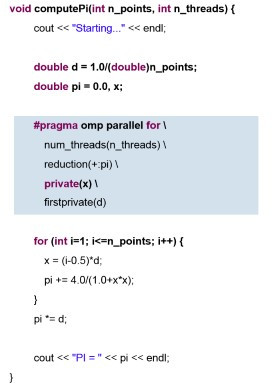
\includegraphics[scale = 1.8]{img/pi computation.jpg}
        \label{pi_computation}
\end{figure}


\colorbox{yellow}{\underline{Example}} (Mandelbrot set): the Mandelbrot set is the set $c$ of complex numbers such that the following function does not diverge:

$$
\begin{cases}
	z_0 = 0 \\
	z_{k + 1} = z_k^2 + c
\end{cases}
$$

The issues about this example are that the number of iterations $k$ is unknown, and the overall computation could lead to potential load imbalance, i.e. it can create very short or very long tasks! Picture \ref{mandelbrot} shows the parallel computation of the Mandelbrot set.

\begin{figure}[h!]
		\centering
		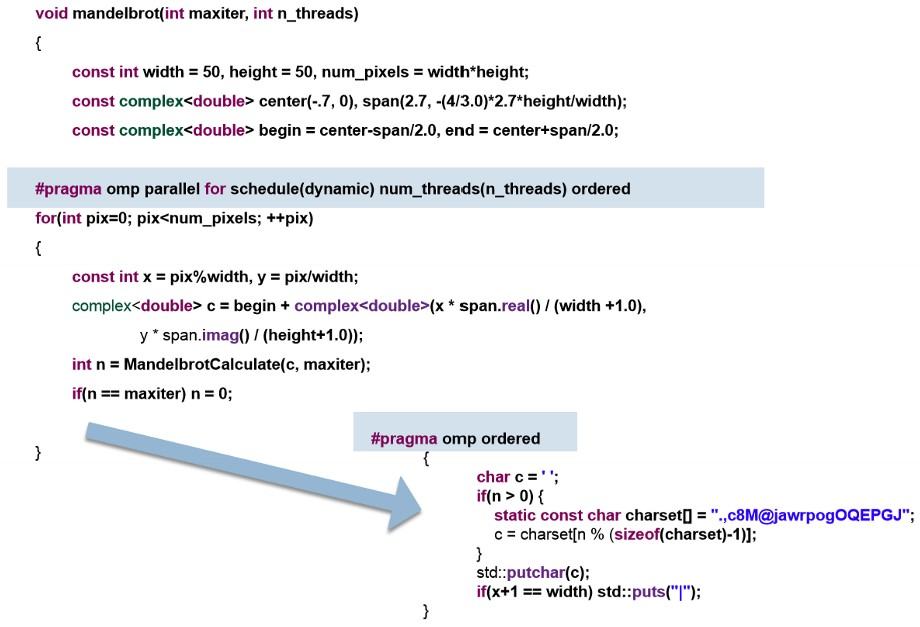
\includegraphics[scale = 1.6]{img/mandelbrot.jpg}
        \label{mandelbrot}
\end{figure}

As we can see:

\begin{itemize}
    \item the schedule is \textit{dynamic}, since the function could have some load imbalance;
    \item the \textit{ordered} directive is used for the output of the points, since we have some constraints in their order.
\end{itemize}


\subsection{OpenMP and Cache}
Once we introduced the OpenMP library, we can now analyze in detail some of its results when used for solving some classic problems. For example, if we consider again the \textbf{matrix multiplication problem}, we can compare the sequential and the parallel computation.

If we consider the sequential computation, showed in Picture \ref{sequential}, we see that each of the three for loops can be parallelized.

\begin{figure}[h!]
		\centering
		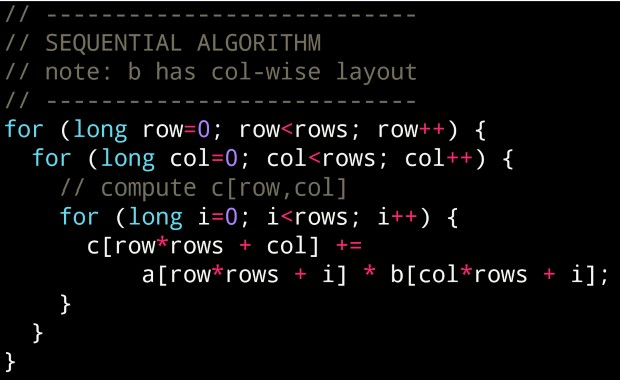
\includegraphics[scale = 1.6]{img/sequential.jpg}
        \label{sequential}
        \caption{Sequential algorithm}
\end{figure}

Intuitively, if we parallelize the most external loop, then $10$ threads are created; if we parallelize the central loop, then $10$ threads are created for each external loop, so $10*N$ threads, where $N$ is the number of rows; finally, if we parallelize the most internal loop, $10*N^2$ threads are created. 

More specifically, by parallelizing the external loop, a thread is created for each row of the matrix $A$, and it scans the full $B$ before writng a new row in $C$: from the point of view of the cache this is quite bad, since the matrix $B$ usually does not fit entirely in the memory. 

On the other hand, if we parallelize the central loop, a thread is created for each column of matrix $B$, and it writes a column in $C$. The advantages of this approach are:

\begin{itemize}
    \item differently from the previous case, not the entire matrix $A$ needs to be stored in memory, but only one row, since all the threads will access the same row for computing a column of $C$. Thus, this approach is very nice since it is characterized by a great cache locality;
    \item each thread computes one column at at time, so we only need to store one column for each thread, which is better for the cache.
\end{itemize}

On the other hand, the main disadvantage of this approach is that the threads are created and destroyed multiple times, resulting in a quite high overhead. Finally, the last approach is to parallelize the internal loop: the code is provided in Picture \ref{par3}.

\begin{figure}[h!]
		\centering
		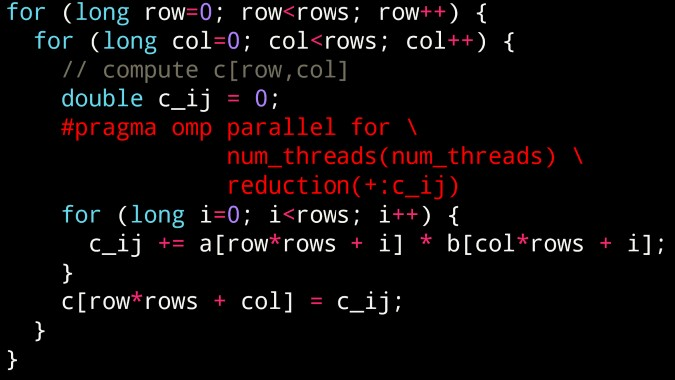
\includegraphics[scale = 1.6]{img/par3.jpg}
        \label{par3}
        \caption{Parallel algorithm: third strategy}
\end{figure}

As we can see, the count variable $c_{ij}$ is used to store the partial sums, and it is updated by each thread independently. In this sense, the parallelization is applied at single row and single column level. From the point of view of the cache, we only need to store one row and one column at a time, and this is very nice, but on the other hand the threads are created and destroyed $N^2$ times, so there's a huge overhead due to thread management.

The resulting execution times were:

\begin{itemize}
    \item 11,500ms for the sequential computation;
    \item 800-1,200ms for the first version of the parallel computation;
    \item 700-6,000ms for the second version of the parallel computation;
    \item 153,923ms for the last version of the parallel computation.
\end{itemize}

In general, we notice a sort of \textbf{instability} in the timings, and this phenomenon is due to the fact that threads can be rescheduled to a different core/processor, and in this case the thread is moved to a different core (or CPU) along with all the data. This phenomenon leads to many cache misses and to a significant decay of the performances, and it can be solved by forcing the threads to not move along the cores, by using the command \textit{export OMP\_PROC\_BIND = true}.

However, we notice that the second strategy is the one that better performs for our task. Now the goal is to \textbf{reduce the thread management overhead}, since, as we underlined before, the threads are created and destroyed multiple times (in particular, once for each row). A solution for this problem is given by switching the first and the second loop: in this case, each thread of the column is destroyed after all the rows of $A$ are scanned, but in terms of the cache this is worse, since we need now to store the matrix $A$ entirely. The code is showed in Picture \ref{par4}.

\begin{figure}[h!]
		\centering
		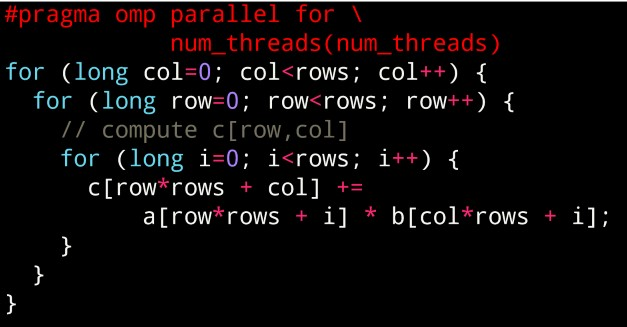
\includegraphics[scale = 1.6]{img/par4.jpg}
        \label{par4}
        \caption{Parallel algorithm: inverted strategy}
\end{figure}

A possible improvement to this implementation is showed in Picture \ref{par5}.

\begin{figure}[h!]
		\centering
		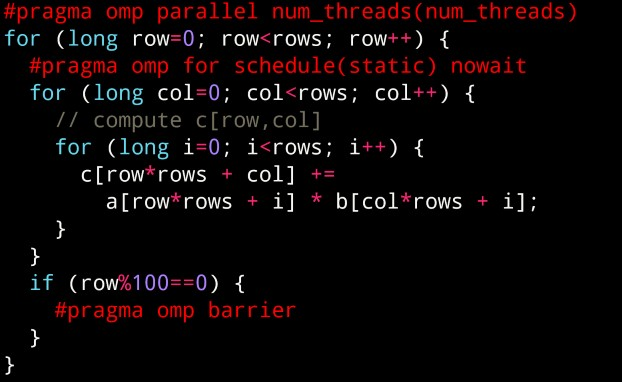
\includegraphics[scale = 1.6]{img/par5.jpg}
        \label{par5}
        \caption{Parallel algorithm: synchronized strategy}
\end{figure}

As we can see, first of all the loop is statically split into chunks, and the \textit{nowait} directive means that once a thread has completed the row, it moves to the following one, resulting in an increased number of rows that are processed simultaneously. Moreover, this approach results in less synchronization overhead and, potentially, in a better use of the cache; however, on the other hand, this reduction of synchronization could result in no cooperation between threads (so in less cache hits) and could lead to situations in which the data do not fit into the cache. For these reasons, a thread synchronization is performed after 100 rows of $A$ (note that this quantity depends on the cache memory that is available).

The timings for the strategy we described above are:

\begin{itemize}
    \item 810ms for the inverted strategy;
    \item 348ms for the synchronized strategy.
\end{itemize}

In particular, recalling that the time for the sequential implementation was 11,500ms, we notice that using the synchronized strategy we reach a speedup of $\frac{11,500}{348} = 33$, which is a great result.

\subsection{\textit{perf}}
The Linux OS provides the \textit{perf} command for profiling the execution of a given program, and in particular it allows to measure the number of misses for each level of the cache, the percentage of misses etc..

\section{Patterns of Parallelism}\label{ch4}
In general, there exist some frequent \textbf{patterns of parallelism}, but we may need to design something quite specific for our problem/algorithm. We might identify two main techniques:

\begin{itemize}
    \item \textbf{decomposition techniques} (like \textit{divide-and-conquer}) that are used to generate (possibly) \textbf{independent sub-problems} that can be run in \textbf{parallel}. Notice that usually this is not a simple task, and also the merging phase of the outputs could be a problem;
    \item \textbf{mapping techniques} to decide who is going to execute what. These techniques depend on the \textbf{dependencies} among the tasks to be performed and their goal is to \textbf{maximize the load balance}.
\end{itemize}

\subsection{Task dependency graph (TDG)}
In general, the decomposition can be modelled with a \textbf{Task Dependency Graph} or \textbf{TDG}, which is a direct acyclic graph (DAG) where each \textbf{node} corresponds to a \textbf{task}, the \textbf{edges} represent task/data \textbf{dependencies} and the labels on the nodes measure the task computational cost.

\begin{figure}[h!]
		\centering
		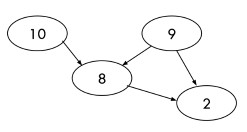
\includegraphics[scale = 2.0]{img/tdg.jpg}
        \label{tdg}
        \caption{Example of TDG}
\end{figure}

In this sense, the TDG is used to show the relationships between the tasks resulting from a decomposition, and is not unique for a given problem: each problem could have different decompositions, task size etc.., i.e. the TDG depends on the specific decomposition of the problem. Moreover, TDG can be used for discovering load balance and the order of execution of the tasks.

Now, we define \textbf{parallelism degree} the number of tasks that can be executed in parallel. Notice that this number may change during the execution of an application, but in general it increases with a fine-grained decomposition. Obviously, our goal is to obtain an high parallelism degree, in order to better exploit threads and parallel computations.

A \textbf{directed path in a TDG} is a sequence of tasks in the TDG (which cannot be executed in parallel) linked by a dependency relation. The length of the path is given by the sum of the weights (i.e. labels) of its nodes.

A \textbf{critical path} is the longest directed path in the TDG, and it represents the \textbf{bottleneck} of the application. In this sense, in represents the minimum execution time, i.e. $\text{total running time} \geq \text{critical path}$.

Finally, the \textbf{average parallelism degree} is defined as $\frac{\text{Total work}}{\text{Length of the critical path}}$, where Total work represents the sum of all the labels of the graph. This measure provides an estimation of how much work we can run in parallel, so the larger the result, the more work we can run in parallel. Our goal is to define a TDG with the shortest possible critical path, in order to maximize the work that can be done in parallel.

\subsection{Task interaction graph (TIG)}
In this case, the nodes represent the tasks, the edges represent interaction/data exchange, the node labels represent the computational cost and the edge labels represent the amount of data that is exchanged.

\begin{figure}[h!]
		\centering
		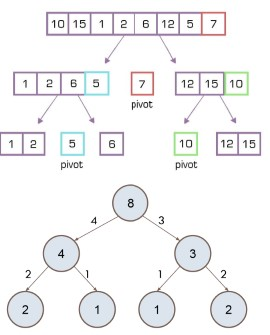
\includegraphics[scale = 2.0]{img/tig.jpg}
        \label{tig}
        \caption{Example of TIG}
\end{figure}

Our goal is to find the minimum cut (i.e. the cut with minimum weight) s.t. each partition has the same load.

\subsection{Mapping}
In general, the number of tasks exceeds the number of processors, so we have a \textbf{mapping problem}, i.e. we have to assign the tasks to the processors. Usually, this mapping is planned on the basis of TDG and TIG:

\begin{itemize}
    \item TDG helps in achieving load balance and minimizing waiting times (each processor receives the same load);
    \item TIG minimizes the interactions/communications between tasks (useful in a distributed environment).
\end{itemize}

Clearly, there can be a conflict between these two goals, but in general the \textbf{guidelines} are the following:

\begin{itemize}
    \item Assign independent tasks to different processors;
    \item Tasks on the critical path must be assigned as early as possible;
    \item Minimize the interaction/communication costs by scheduling "dense" sub-graphs of the TIG to the same processor.
\end{itemize}

We will now focus on some common patterns of parallelism:
\begin{itemize}
    \item Pipeline;
    \item Single Program Multiple Data / Data Parallel;
    \item Task Pool;
    \item Dynamic Task Creation.
\end{itemize}

\subsubsection{Pipeline}
A \textbf{pipeline} is a special kind of task-parallelism, where the \textbf{computation} is \textbf{partitioned} into stages that are executed sequentially: the output of a stage provides the input of the following one. 

\begin{figure}[h!]
		\centering
		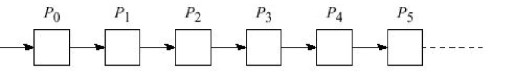
\includegraphics[scale = 2.0]{img/pipeline1.jpg}
        \label{pipeline1}
        \caption{Pipeline}
\end{figure}

\textbf{Asymptotically}, a pipeline achieves a speed-up equal to the number of stages. If we have $p$ processors, an input stream of $n$ elements and a cost of each task of $t$, then:

\begin{itemize}
    \item $(p-1)$ steps are used to fill the pipeline, in $(p-1)t$ time;
    \item $n$ steps are used to produce the output, in $nt$ time (each stage of the pipeline must be processed);
    \item The total speedup is $\frac{\text{sequential time}}{\text{parallel time}} = \frac{ptn}{nt + (p-1)t} = \frac{p}{1 + \frac{p-1}{n}} \rightarrow p$
\end{itemize}

In this sense, if each stage has the same load of work, then we reach a \textbf{linear speedup}.

\begin{figure}[h!]
		\centering
		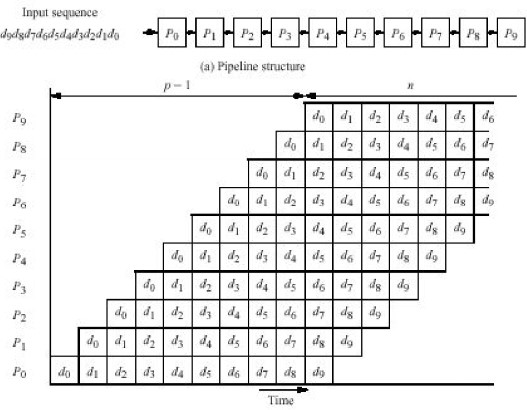
\includegraphics[scale = 2.0]{img/pipeline2.jpg}
        \label{pipeline2}
        \caption{Execution of a pipeline}
\end{figure}

\subsubsection{Single Program Multiple Data}
This strategy addresses to problems that can be solved with a large set of completely independent sub-tasks, i.e. in case of a completely disconnected TDG. Clearly, this is not a common scenario, but for example involves the Mandelbrot problem.

\begin{figure}[h!]
		\centering
		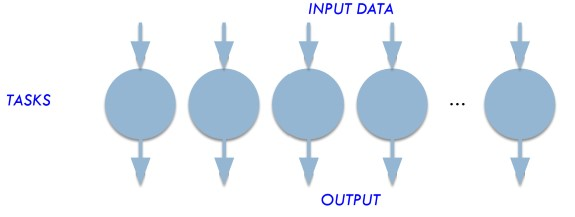
\includegraphics[scale = 1.5]{img/SPMD.jpg}
        \label{spmd}
        \caption{Single Program Multiple Data}
\end{figure}

\subsubsection{Task Pool}
In this case the task list is stored in a shared data structure, we have a fixed number of threads and each thread dynamically picks a task and executes it. Clearly, this technique is characterized by a synchronization overhead, and a thread may possibly generate a new task too.

\begin{figure}[h!]
		\centering
		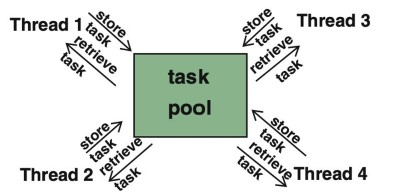
\includegraphics[scale = 1.7]{img/task pool.jpg}
        \label{task pool}
        \caption{Task Pool}
\end{figure}

In the Mandelbrot problem, there's a static partitioning of the input, assigning one pixel per task, then each thread processes a portion of the input, with dynamic assignment.

\subsubsection{Dynamic Task Creation}
In this technique, each thread can dynamically create new tasks, and it is useful to:

\begin{itemize}
    \item Improve the \textbf{parallelism degree};
    \item Adapt to task of unknown costs, since it can split a long task into smaller ones;
    \item Adapt to non uniform resources, since it can exploit multiple machines with different computing power.
\end{itemize}

Notice that a \textbf{task queue} must be shared among a pool of threads. This technique is very common, since it allows to deal with very different tasks.

\textbf{Distributed Load Balancing}

The goal of this approach is to remove centralization, i.e. remove the concept of \textit{master node}, and to favor data exchange among neighbors. There exist two different variant for this technique:

\begin{itemize}
    \item Push/Sender-Initiated, in which the worker that generates a new task sends it to another worker, instead of putting it in the task list;
    \item Pull/Receiver-Initiated, in which when a worker is idle, it asks other workers for a job to execute (work stealing)
\end{itemize}

\begin{figure}[h!]
		\centering
		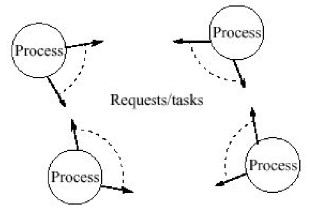
\includegraphics[scale = 2.0]{img/distributed load balancing.jpg}
        \label{distr load balancing}
        \caption{Distributed Load Balancing}
\end{figure}

In the Push/Sender-Initiated, the worker to which the task is sent can be selected:

\begin{itemize}
    \item At \textbf{random}, among all the workers;
    \item \textbf{Global Round Robin (GRR)} in which a global random variable/marker points to the "next" worker, and a worker needing a partner reads and increments the global variable;
    \item \textbf{Local Round Robin (LRR)}, in which each processor keeps a private pointer to the next available worker, so there's no overhead due to sharing a global variable.
\end{itemize}

In general, the choice among \textbf{static mapping} (pipeline, single program multiple data) and \textbf{dynamic mapping} (task pool, dynamic task creation) can be made according to the following schema:

\begin{figure}[h!]
		\centering
		\includegraphics[scale = 1.8]{img/dynamic vs static mapping.jpg}
        \label{dy vs st}
        \caption{Static vs dynamic mapping}
\end{figure}

In general, the \textbf{static mapping} is preferable, since is does not need any synchronization.

\subsection{Prefix sum}
Given a list of integers $x_0, x_1, .., x_{n-1}$, compute the partial sum up to index $i$, for each $i$. 

The optimal sequential algorithm has complexity $O(n)$: for ($i$ = 1; $i<n$; $i++$) : $x[i] += x[i-1]$.

However, this algorithm is difficult to be parallelized, since each iteration depends on the previous one. For example, we cannot split the vector $x$ into two parts $T_1$ and $T_2$, since $T_2$ must wait $T_1$ to perform its computations. For this reason, the naive parallel algorithm works as follows:

\begin{itemize}
    \item Break the dependencies through a step-wise algorithm;
    \item One thread computes one element at each step.
\end{itemize}

\begin{figure}[h!]
		\centering
		\includegraphics[scale = 1.6]{img/parallel prefix sum .jpg}
        \label{parallel prefix sum}
        \caption{Parallel prefix sum}
\end{figure}

In this case:

\begin{itemize}
    \item The total amount of work is $O(N \log N)$, where $\log N$ is the number of steps of the algorithm, and $N$ is the length of the vector. In the sequential version, the amount of work was $O(N)$;
    \item The complexity is $O(\log N)$, while in the sequential algorithm we had $O(N)$.
\end{itemize}

As we can see, in this case the parallel version of the algorithm is quite different from the sequential one, and we also notice that the parallel version results in more work to be done, but the execution time is faster. For this reason, in this case the benefits of the parallel algorithm can be obtained only if enough processors are available, otherwise it is better to execute the sequential algorithm.

\begin{figure}[h!]
		\centering
		\includegraphics[scale = 1.6]{img/prefix sum algo.jpg}
        \label{prefix sum algo}
        \caption{Implementation of the parallel algorithm}
\end{figure}

For this reason, now our goal is to \textbf{reduce the amount of work}, i.e. number of sums, in order to reduce the number of processors that are needed for the parallelization.

The idea is to focus on an \textbf{exclusive prefix sum}, i.e. a prefix sum that discards the last element, which is composed on two phases: the \textbf{Up-sweep} phase and the \textbf{Down-sweep} phase. 

\begin{figure}[h!]
		\centering
		\includegraphics[scale = 2.0]{img/up-sweep.jpg}
        \label{up-sweep}
        \caption{Up-sweep phase}
\end{figure}

On the one hand, the goal of the \textbf{Up-sweep} phase is to store in a vector some important partial sums. In particular, it performs $N-1$ summations in $\log N$ steps, and the resulting vector contains several \textbf{correct partial sums}, together with elements for which the prefix sum is not computed. In this sense, an important property of the resulting vector is that each node that contains the correct partial sums holds the \textbf{sum of its children}.


\begin{figure}[h!]
		\centering
		\includegraphics[scale = 2.0]{img/down-sweep2.jpg}
        \label{down-sweep}
        \caption{Down-sweep phase}
\end{figure}

On the other hand, the idea of the \textbf{Down-sweep} is to enforce the property that \textbf{each node should have the sum of all the leaves preceding it}, i.e. before its leftmost child. This means that:

\begin{itemize}
    \item The root has value 0;
    \item A \textbf{left} child has the same predecessors of its parent, so it has the \textbf{same value as it's parent};
    \item A \textbf{right} child is preceded by its parent predecessors plus the sibling's children, so its value should be equal to its \textbf{parent plus the up-sweep value of its sibling}.
\end{itemize}

This phase takes $\log N$ steps and $N-1$ summations, so the overall algorithm:

\begin{itemize}
    \item Has  complexity of $O(\log N)$ (i.e. number of steps);
    \item Performs $O(N)$ summations (amount of work), which is much less that the previous parallel version of the algorithm. Moreover, notice that a large parallelism degree can be exploited for most steps.
\end{itemize}

Picture \ref{gpu} shows the performances of the sequential algorithm (CPU), the naive parallel algorithm (Naive) and a version of the algorithm running on graphic processors (CUDA).

\begin{figure}[h!]
		\centering
		\includegraphics[scale = 1.5]{img/gpu perf.jpg}
        \label{gpu}
        \caption{GPU performance}
\end{figure}

\subsection{QuickSort}
We now focus on the problem of parallelizing the \textbf{QuickSort} algorithm.

\begin{figure}[h!]
		\centering
		\includegraphics[scale = 2.0]{img/quicksort.jpg}
        \label{quicksort}
        \caption{QuickSort algorithm}
\end{figure}

A naive approach would be of running step (a) as 1 sequential task, step (b) as 2 parallel tasks, step (c) as 4 parallel tasks, and so on.., until the number of tasks is equal to available parallelism. However, this approach, and in general this algorithm, could lead to two important \textbf{issues}:


\begin{itemize}
    \item \textbf{Load imbalance}, since the pivot does not split the array in a balanced way, so the recursion in one side could complete the computation before the recursion in another side. In other words, the array subsequences depend on the pivot selection, and different lengths lead to different workloads and imbalance.
\end{itemize}

We now focus on different techniques for parallelizing the QuickSort algorithm.

\subsubsection{Local and global arrangement}
The first method works as follows:

\begin{enumerate}
    \item Split the input array into several sub-arrays, and assign each of them to a processor;
    \item Pick a pivot;
    \item \textbf{Local arrangement}: separate each sub-array according to the chosen pivot;
    \item \textbf{Global arrangement}: separate the global array according to the chosen pivot;
    \item Recursively on the two sub-arrays until each processor can use a sequential algorithm to sort its sub-array.
\end{enumerate}

\begin{figure}[h!]
		\centering
		\includegraphics[scale = 2.0]{img/parallel quicksort.jpg}
        \label{quicksort par}
        \caption{Parallel QuickSort algorithm}
\end{figure}

This method suffers from the following \textbf{disadvantages}:

\begin{itemize}
    \item It requires a very high \textbf{parallelism degree};
    \item The \textbf{load balance} is still sensitive to the pivot selection.
\end{itemize}

\subsubsection{Odd-Even transposition}
This method works as follows:

\begin{enumerate}
    \item Repeat $\frac{n}{2}$ times:

    \begin{enumerate}
        \item Compare-exchange the \textbf{odd} elements with their immediate neighbor;
        \item Compare-exchange the \textbf{even} elements with their immediate neighbor.
    \end{enumerate}
\end{enumerate}

\begin{figure}[h!]
		\centering
		\includegraphics[scale = 2.0]{img/odd-even transposition.jpg}
        \label{odd-even}
        \caption{Odd-even transposition}
\end{figure}

Clearly, the \textbf{sequential} complexity is $O(n^2)$, so it is a bad sequential algorithm. On the other hand, each phase can be easily \textbf{parallelized}, and if the number of processors $p = \frac{n}{2}$, then each phase (compare odd or compare even) takes $O(1)$, so in total $O(n)$, so the overall complexity is $\frac{n}{2} * n = O(n^2)$. Since the complexity of sorting is $O(n \log n)$, this algorithm is not cost optimal.

However, this algorithm can be generalized by assigning batches of $n/p$ elements to each processor. In this case, the local sort on $n/p$ elements (i.e. the sort of each batch) takes $p (n/p \log (n/p)) = O(n \log (n/p))$, so in order to produce the result we need a linear scan of all the batches for each phase, so the cost is $p (p * n/p) = O(np)$. If $p = O(\log n)$, then the parallel algorithm is cost optimal with cost $O(n \log n)$. However, this strategy has the drawback that when increasing $p$, we must exponentially increase $n$ in order to have the same scalability, otherwise the algorithm would not be cost optimal anymore.

\subsection{Bitonic sort}
We now focus on another type of sort, and we will discuss a sequential algorithm which is not optimal, but easily to be parallelized (with an high parallel degree too).

A sequence $X = x_1, x_2, .., x_N$ is said to be \textbf{bitonic} if $x_1, .., x_j$ is \textbf{monotonically increasing} and $x_{j+1}, .., x_N$ is \textbf{monotonically decreasing}, or this holds for a cyclic shift of the input sequence.

\begin{figure}[h!]
		\centering
		\includegraphics[scale = 2.0]{img/bitonic sequence.jpg}
        \label{bitonic seq}
        \caption{Examples of bitonic sequences}
\end{figure}

We now address two problems:

\begin{enumerate}
    \item How to sort a bitonic sequence?;
    \item Supposing that we can sort a bitonic sequence, how can we make a sequence bitonic?
\end{enumerate}

\subsubsection{Bitonic sort}
A \textbf{comparator} $[i:j]$ sorts the i-th and the j-th element of a sequence into a non-decreasing order. A \textbf{Bitonic split} is the result of applying N/2 comparators of the kind $[i:i + N/2]$ for $1 \leq i \leq N/2$ to a \textbf{bitonic sequence}. Picture \ref{bitonic split} shows the functioning of a bitonic split.

\begin{figure}[h!]
		\centering
		\includegraphics[scale = 2.0]{img/bitonic split.jpg}
        \label{bitonic split}
        \caption{Functioning of a bitonic split}
\end{figure}

The Bitonic split ensures two properties:

\begin{itemize}
    \item All the elements of the first half are less or equal the elements of the second half: if $Z = BS(X)$, i.e. $Z$ is the result of the Bitonic split of the input $X$, then:

    $$
    Z_1, .., Z_{N/2} \leq Z_{N/2 + 1}, .., Z_N
    $$

    \item Each of the halves is a bitonic sequence, i.e. $Z_1, .., Z_{N/2}$ and $Z_{N/2 + 1}, .., Z_N$ are bitonic.
\end{itemize}

Both the properties hold since the input sequence is bitonic.

Now, the idea of the algorithm is to \textbf{recursively} apply a \textbf{Bitonic split} to \textbf{each of the sequences}. Thus, a \textbf{Bitonic merge} performs recursive Bitonic splits until the resulting sequence is sorted in increasing order.

\begin{figure}[h!]
		\centering
		\includegraphics[scale = 2.0]{img/bitonic merge.jpg}
        \label{bitonic merge}
        \caption{Functioning of a bitonic merge}
\end{figure}

This method involves $\log N$ steps (where $N$ is the length of the input sequence), and each step performs $N/2$ compare/swap operations (i.e. bitonic splits). Thus, the \textbf{complexity of the sequential algorithm} is $O(N \log N)$.

If we have $N/2$ processors, than each comparison can be executed in parallel, so the \textbf{complexity of the parallel algorithm} is $O(\log N)$.

Before focusing on how we can make a sequence bitonic, we now discuss an interesting \textbf{property} of this algorithm. Indeed, in this method the \textbf{operations do not depend on the input data}, so the algorithm works for every input, provided that it is bitonic. Notice that this is a very good advantage, since it makes the algorithm easily parallelizable, exploiting an high parallelism degree. Notice also that this property does not hold for every algorithm, e.g. the operations of the QuickSort algorithm depend on the choice of the pivot.

\subsubsection{Constructing a Bitonic sequence}
In order to feed the final Bitonic Merge step with a bitonic sequence, the two halves of the input are sorted ascendingly/descendingly by recursively invoking Bitonic sort. 

\begin{figure}[h!]
		\centering
		\includegraphics[scale = 2.0]{img/bitonic sort.jpg}
        \label{bitonic sort}
        \caption{Functioning of a bitonic merge}
\end{figure}

As we can see, there are $\log N$ Bitonic merge phases, each having complexity $N \log N$, so the overall complexity id $O(N \log^2 N)$. Notice that the Bitonic sort can be parallelized very well, and it can exploit a large parallelism degree. The parallel cost is $O(p \log^2 N)$, so it is not cost optimal, and this algorithm is very popular for GPUs and for medium sized inputs.

\section{Large-scale data processing with MapReduce}
When we have a lot of data, we must exploit multiple machines, so larger architectures that support parallelization, both on the computation and on the read/write operations. In this sense, some standard architectures are \textbf{commodity clusters}, which are standard servers that scale the computation up on different machines, and \textbf{Gigabit Ethernet interconnections.}

\subsection{Commodity clusters}

\begin{figure}[h!]
		\centering
		\includegraphics[scale = 2.0]{img/cluster.jpg}
        \label{cl arch}
        \caption{Cluster architecture}
\end{figure}

As we can see, two main failures may happen:

\begin{itemize}
    \item A failure in the \textbf{network}, after which some nodes are not reachable anymore;
    \item A failure on a \textbf{machine}.
\end{itemize}

In general, handling failures is difficult, since they're extremely frequent, so an important property of the cluster is to be \textbf{failure resilient}. In particular, if we address the problem of a \textit{machine failure}, we have a solution represented by the \textbf{Distributed File System}, which provides a global file namespace and it supports huge files (100 of GBs to TBs): in this case, data is rarely updated in place, and \textbf{reads} and \textbf{appends} are common. Some examples of such DFS are \textit{Google GFS} and \textit{Hadoop HDFS}

In particular, the Hadoop DFS is composed of the following entities:

\begin{itemize}
    \item \textbf{Chunk servers}, which contain the splitted file and serve the \textit{master node}. Each chunk is typically 16-64MB, and it is replicated 2x or 3x, so the \textbf{replication} is at \textbf{chunk level}. Note that the HDFS tries to keep the replicas in different racks;
    \item \textbf{Master node} (or \textbf{Name node}), which stores all the metadata and takes care of giving the user a unique FS, and it keeps track of all the chunk servers. The mater node might be replicated;
    \item Client library for file access, which talks to the master node to find the chunk servers and connects directly to chunk servers to access data.
\end{itemize}

The operations that are supported by the HDFS are \textbf{concurrent reads} and \textbf{single write} operations, which are implemented as append operations.

Two very important files in the HDFS are:

\begin{itemize}
    \item The \textbf{sequence file}, which is persistent data structure for binary key-value pairs. This file can be written only by using the \textit{append()} method, and can be read only by using the \textit{next()} method;
    \item The \textbf{map file}, which represents a higher-level file and it is a \textbf{sorted sequence file} with an \textbf{index} to support lookups by key. Thus, in this case the file can be read by using \textit{next()} or \textit{get()} (by key). Notice that the lookup by key is implemented with two sequence files: \textit{Index} and \textit{Data}, where the \textit{Index} file must be loaded in memory for random lookups.

    \begin{figure}[h!]
		\centering
		\includegraphics[scale = 2.0]{img/index map file.jpg}
        \label{sequence map files}
        \caption{\textit{Index} and \textit{Data} files}
    \end{figure}
\end{itemize}

Finally, notice that the \textbf{replication of data three times} is a robust guard against loss of data due to uncorrelated node failures: for a large cluster, the probability of losing a block during one year is less than 0.005. The key understanding is that about 0.8 percent of nodes fail each month, so for the sample of large clusters, a node or two is lost everyday.

\subsection{MapReduce}
\textbf{MapReduce} represents a "novel" programming paradigm, which is based on top of \textit{<key,value>} pairs, where the \textit{keys} and the \textit{values} are \textbf{user-defined}, so they can have any type. This framework is essentially based on two functions:

\begin{itemize}
    \item \textbf{Map}, which takes as input a key-value pair $(k_1, v_1)$, and produces as output an intermediate data $v_2$ labeled with a key $k_2$:

    $$
    \text{Map}(k_1, v_1) = \text{list}(k_2, v_2)
    $$
    
    \item \textbf{Reduce}, which given every data $\text{list}(v_2)$ associated with a key $k_2$ (so we suppose that we can execute multiple \textit{Map} operations on the same data), it produces the output of the algorithm $\text{list}(k_3, v_3)$, so its functioning is pretty similar to a GroupBy.

    $$
    \text{Reduce}(k_2, \text{list}(v_2)) = \text{list}(k_3, v_3)
    $$
\end{itemize}

If we put all in parallel, we have a set of \textbf{mappers} and a set of \textbf{reducers}:

\begin{enumerate}
    \item A \textbf{mapper} processes only a split of the input, which may be distributed across several machines;

    $$
    \text{Map}(k_1, v_1) = \text{list}(k_2, v_2)
    $$
    
    \item A \textbf{shuffle} phase transfers the data associated with a given key from the \textit{mappers} to the proper \textit{reducer}, so that the reducer will receive data sorted by key;
    \item A \textbf{reducer} produces only a portion of the output associated with a given set of keys. Notice that \textit{reducers} can run in parallel.

    $$
    \text{Reduce}(k_2, \text{list}(v_2)) = \text{list}(k_3, v_3)
    $$
    
\end{enumerate}

\underline{Example: WordCount using MapReduce}

Picture \ref{wc code} show the code of the Map and Reduce functions for the word count problem.

\begin{figure}[h!]
		\centering
		\includegraphics[scale = 2.0]{img/word count code.jpg}
        \label{wc code}
        \caption{Map and Reduce functions for word count problem}
\end{figure}

As we can see, the Map function produces a (word,1) pair for each of the word in the document, while the Reduce function receives in input a word and a list of 1's, and produce in output a (word,count) pair.

Picture \ref{wc scheme} shows the execution of the MapReduce framework for word counting.

\begin{figure}[h!]
		\centering
		\includegraphics[scale = 2.0]{img/word count scheme.jpg}
        \label{wc scheme}
        \caption{Execution scheme of MapReduce for word counting}
\end{figure}

As we can see, the text is splitted into 3 chunks: the Map function of each chunk produces a (word,1) pair for each word of the input. Then, the Shuffle phase implements a GroupBy over the output of the Map functions, and produces a pair composed by a word and a list of 1's, which represents the input of the Reduce function. Finally, the output provides the count for each word of the input. Notice that the only operations that the user has to implement are the one from the Split phase to the Map phase, and from the Shuffle phase to the Reduce phase, since all the others belong to the MapReduce framework.

\subsubsection{Architecture}

Picture \ref{mr arch} shows the general architecture of the MapReduce framework.

\begin{figure}[h!]
		\centering
		\includegraphics[scale = 2.0]{img/map reduce arch.jpg}
        \label{mr arch}
        \caption{MapReduce architecture}
\end{figure}

\begin{enumerate}
    \item The \textit{user program} invokes the MapReduce;
    \item The \textit{master node} coordinates the work. In particular, it assigns the \textit{workers} the splitting to which performing the Map function, and to other \textit{workers} the splitting to which performing the Reduce function and what intermediate files to read. The assignment of the chunks is usually based on the machine in which the chunk itself resides;
    \item The \textit{Map workers} read the split of the input files and they execute the Map function, writing the (key,value) output pairs into intermediate files in the local File System;
    \item The \textit{Reduce workers} read the intermediate files from the FS and execute the Reduce function, writing the final result into output files, which in turn can represent the input of another Map function.
\end{enumerate}

\subsubsection{Coordination and failures}
The coordination between all the workers is ensured by the \textbf{master node}. This data structure maintains the \textit{status} for each of the tasks (idle, in-progress, completed), and idle tasks get scheduled as workers become available. Moreover, when a Map task completes, it sends the master the location and size of its $R$ intermediate files, one for each reducer, and the master pushes these info to the reducers. Finally, another task of the master is to periodically ping the workers to detect failures.

A \textbf{failure} may happen on Map workers, on Reduce workers and on the Master node:

\begin{itemize}
    \item If a \textbf{Map worker failure} happens, then the Map tasks that are completed or in-progress are reset to idle, and the Reduce workers are notified when the task is rescheduled on another worker, in order to delete his local copy of the failed Map's data;
    \item If a \textbf{Reduce worker failure} happens, then only the in-progress tasks are reset to idle, since the results of the completed tasks are already saved in the distributed FS;
    \item If the \textbf{Master node} fails, then the MapReduce task is aborted, and the client is notified.
\end{itemize}

\subsubsection{Number of Map and Reduce jobs}
In general, we number $M$ of map tasks and $R$ of Reduce tasks are parameters to be tuned. A rule of thumb suggests that $M$ and $R$ should be larger than the number of nodes in the cluster, otherwise we would not exploit the parallelization. In general:

\begin{itemize}
    \item $M$ is determined by the number of input splits;
    \item $R$ is determined by the number of distinct key-value pairs, so on the data;
    \item Having several mappers and reducers may improve load balancing and it speeds the recovery from work failure, but on the other hand it increases the overhead given by the coordination between the different workers;
    \item Usually $R < M$, because the system has a maximum capacity of parallel reducers, so the reducers are executed in waves. The shuffling of the first wave is done in parallel with mappers, i.e. very early in the computation, but the shuffling of other waves is done later, so there's less communication/computation overlap.
\end{itemize}

\subsubsection{Some improvements}
Some improvements over the classic architecture of Picture \ref{mr arch} can be done:

\begin{itemize}
    \item We know that Map tasks on the same node will produce many pairs with the same key (an example is provided in Picture \ref{wc scheme}, where we have a node containing two pairs \textit{(Car, 1)}), so the idea is to save some network time by pre-aggregating the pairs at Map level by using the \textbf{combiners}. In this sense:

    $$
    \text{combine}(k_2, \text{list}(v_2)) = \text{list}(k_3, v_3)
    $$

    In the example, the result of the use of the \textit{combine} function is to have a pair \textit{(Car, 2)} before the shuffling phase. Notice that the \textit{combine} functionality usually exploits the Reduce function, if the Reduce function is commutative and associative.

    \item We know that the input of the Map tasks are created by contiguous splits of the input file, and for the Reducer we need to ensure that intermediate \textit{(k,v)} pairs with the same key end up at the same reducer. In this sense, the system uses a default \textbf{partition function}, e.g. $\text{hash}(key) \text{mod} R$, in order to ensure both a faster computation of the Reduce functions and load balance among the reducers. Notice that the partition functions may be overridden and customized.

    \item In order to shorten the total execution time and to ensure fault tolerant property of the system, the system enables the \textbf{back-up tasks}, i.e. tasks that are executed twice, in two different machines, and the result of the faster one is kept. This solution dramatically shortens the job completion time.
    
\end{itemize}

In general, it is useful to underline that the MapReduce framework is \textbf{not} adopted for \textbf{performances}, since for example the writes of the mapper to the disk produce a huge overhead, and in general the shuffle step represents the bottleneck of the system. The \textbf{advantage} of this framework is that the user is asked only to override two functions (sometimes, other functions are needed to be implemented, such as combiners, partitioners, etc..), but on the other hand \textbf{not everything can be implemented in terms of MapReduce}. For example, the \textit{all pairs similarity problem} requires to scan $N^2$ candidates, where $N$ is the number of documents in the collection, and experiments showed that for 60MB worth of documents, the framework would generate 40GB of intermediate data to be shuffled. Graph mining problems such as community detection and PageRank computation are hard problem for MapReduce too.

\subsubsection{Implementations of MapReduce}
There exist many methods for implementing a MapReduce framework:

\begin{itemize}
    \item \textbf{Hadoop}, which is an Apache project providing a Java implementation of MapReduce and relying on the HDFS (Hadoop Distributed File System), which is efficient and reliable. Hadoop only needs to copy Java libraries into each machine of the cluster;
    \item \textbf{Dryad & DryadLINQ};
    \item \textbf{Pig}, which provides a rich scripting language, which is then transformed into a chain of MapReduce jobs;
    \item \textbf{Hive}, which is a open-source data warehousing solution built on top of Hadoop, supporting queries in a SQL-like declarative language;
    \item \textbf{Spark}, which is a fast and general-purpose cluster computing system, that provides a high-level APIs in Scala, Java and Python, that make parallel jobs easy to write. It resolves around the concept of a Resilient Distributed Dataset (RDD), which is a fault-tolerant collection of elements that can be operated on in parallel
\end{itemize}

\subsection{Documents all pairs similarity with MapReduce}
The problem is defined as follows: given a collection of documents and a minimum required similarity threshold, the goal is to retrieve from the collection the number of pairs of documents that have a similarity greater or equal to the threshold value. In this case, each document is represented as a vector $d$ of $N$ elements, where $N$ is the size of the lexicon, and each $d[i]$ stores the \textit{tf-idf} value of term $i$ in the corpus. Moreover, the similarity is computed using the cosine similarity:

$$
s(a,b) = \sum_{i = 1, .., N} a[i] \cdot b[i]
$$

We now discuss a method for solving this problem exploiting the MapReduce framework. 

\subsubsection{First solution}
First of all, we can observe that the minimum requirement for two documents to have a similarity greater than 0 is to have at least one term in common, so the idea is to skip the computation of the similarity for two documents that do not have any term in common. In this sense, if we store, for each term in the lexicon, the list of documents containing that term, we can easily compute the similarity between these documents.

$$
(\text{term}_1, [\text{doc}_1, \text{doc}_2, ..])
$$

Thus, the \textbf{Reduce function} works like this: it receives in input a key-value pair, where:

\begin{itemize}
    \item the key is represented by the term;
    \item the value is represented by the list of documents in which the term appears.
\end{itemize}

, and for each pair of documents in which each term in the lexicon appears, it computes the similarity and it compares it with the threshold value. Thus, it never computes the cosine similarity of documents that do not contain any term in common. 

Once we designed the Reduce function, we must design the Map and the Shuffle functions. The \textbf{Map function} produces, for each term in the lexicon, a key-value pair where:

\begin{itemize}
    \item the key is represented by the term;
    \item the value is represented by a tuple (docID,document), where document represents the full document;
\end{itemize}

Then, the \textbf{Shuffle function} simply performs a GroupBy operations by key, i.e. by term, and it produces the key-value pairs that are given in input to the Reduce function. Picture \ref{mr all pairs} shows the Map and the Reduce functions for this problem.

\begin{figure}[h!]
		\centering
		\includegraphics[scale = 2.0]{img/map reduce all pairs.jpg}
        \label{mr all pairs}
        \caption{Map and Reduce functions for all pairs similarity}
\end{figure}

Picture \ref{mr ex} shows an example of the functioning of the MapReduce framework for this problem.

\begin{figure}[h!]
		\centering
		\includegraphics[scale = 2.0]{img/mr ex.jpg}
        \label{mr ex}
        \caption{Example of MapReduce functioning for all pairs similarity}
\end{figure}

However, a \textbf{first problem} is the following one: if a document has 1,000 terms, then the document is replicated 1,000 times after the Map execution.

\subsubsection{Second solution}
In order to solve the previous problem, we implement the so called \textbf{prefix filtering}. The idea is to reduce the number of terms we consider, in order to reduce the number of pair for which the similarity is computed.

\begin{enumerate}
    \item First of all, if we consider the term-document matrix, we sort the terms by decreasing score in the corpus, i.e. $d[0]$ corresponds to the term having the largest score of \textit{tf-idf};
    \item Then, we create the \textit{maximum document} d*, i.e. $d^*[i] = \max d[i]$ for each $d$ in the collection. In other words, $d^*$ stores the maximum score of terms in any document. Now we can have \textbf{two observations}:

    \begin{itemize}
        \item If $\text{sim}(d,d^*) < \text{threshold}$, then $d$ has no similar documents in the corpus. This is true because $d^*$ represents the maximum document, so for sure it does not exist another document $d_j$ s.t. $\text{sim}(d, d_j) \geq \text{threshold}$;
        \item Suppose we arrive at a certain term, and $\text{sim}(d,d^*) < \text{threshold}$: then, we can find another document $d_j$ similar to $d_i$ only if they have a term in common after the term we're now considering, otherwise we now that it does not exist another document $d_j$ s.t. $\text{sim}(d, d_j) \geq \text{threshold}$ form the above observation. In this sense, all the terms up to the current one are useless, so we only consider the other in the Map function. In other words, the Map function only considers the terms $t > b(d)$, where $b(d)$ is the \textit{boundary} of a document s.t.:

        $$
        \sum_{0 \leq t \leq b(t)} d[t] \cdot d^*[t] < \text{threshold}
        $$

        , i.e. the boundary of each document is represented by the largest term for which we have $\text{sim}(doc, d^*) < \text{threshold}$
    \end{itemize}
    
\end{enumerate}

Picture \ref{mr all pairs2} shows the Map and Reduce functions for this version of the solution.

\begin{figure}[h!]
		\centering
		\includegraphics[scale = 2.0]{img/mr ex2.jpg}
        \label{mr all pairs2}
        \caption{Map and Reduce functions for all pairs similarity with prefix filtering}
\end{figure}

However, we have another \textbf{problem}: if two documents share 10 terms after filtering, then their similarity is computed and produced in output 10 times.

\subsubsection{Third solution}
A possible solution for this new problem could be sort the whole output and remove the duplicates, but we can easily notice that it is quite expensive.

For this reason, another approach is based on the following idea: only one Reducer is forced to compute the similarity. However, if the two documents are replicated 10 times with 10 different keys, they may end up in 10 different Reducers, so how do we tell the Reducers whether to compute or not the similarity? A selection mechanism can be exploited, e.g. if the reducer has the key equivalent to the largest item, it can compute the similarity.

\begin{figure}[h!]
		\centering
		\includegraphics[scale = 2.0]{img/mr ex3.jpg}
        \label{mr all pairs3}
        \caption{Map and Reduce functions for all pairs similarity with improved prefix filtering}
\end{figure}

Picture \ref{mr all pairs3} shows the Map and Reduce functions for this version of the solution.

\subsection{Graph mining problem with MapReduce}
We consider an undirected graph, and our goal is to find the \textbf{number of connected components}, possibly exploiting the MapReduce framework. In general, graph mining problems are difficult to be parallelized, because, for example, if we think of the "divide-et-impera" approach, we have to partition the graph (i.e. breaking connected components), run the algorithm on each sub-graph and merge the partial results. In this sense, we now exploit a different paradigm of computation, the \textbf{vertex centric paradigm}.

The idea of this paradigm is to write an algorithm for a node rather than a graph, i.e. we specify what each node has to do. In particular, the sketch of the algorithm is the following:

\begin{itemize}
    \item Each node knows about its neighbors and may hold some additional custom information;
    \item The same computational kernel is executed for each node;
    \item Repeat until convergence.
\end{itemize}

The \textbf{advantages} of of this paradigm are:

\begin{itemize}
    \item It is easier to design a "local" algorithm for a single node, rather than for the entire graph;
    \item We can exploit a large parallelism degree, since each node is independent from the others;
    \item It can be implemented over MapReduce, and there exist some specific frameworks like Spark GraphX.
\end{itemize}

However, a \textbf{disadvantage} is that the local view may lead to sub-optimal results.

\subsubsection{Label propagation}
We now describe the algorithm we introduced in the previous section. 

The \textbf{input} of the algorithm is a list of $(X,C_{\text{min}})$ pairs, meaning that $X$ belongs to the connected component with id $C_{\text{min}}$: clearly, when the algorithm starts, node $X$ belongs to component with id $X$. Moreover, each node knows its neighbors $N(X)$.

The algorithm works as follows:

\begin{enumerate}
    \item Node $X$ sends its own component id $C_{\text{min}}$ to all its neighbors $N(X)$, along with itself. In this sense, each node outputs a $(X, C_{\text{min}})$ pair;
    \item Node $X$ receives a list of component ids and computes the minimum among them, i.e. the new $C_{\text{min}}$;
    \item Repeat until convergence, i.e. when no updates occur.
\end{enumerate}

As we said before, the idea of the algorithm is at each step, each node shares its own information to the neighbors, and the information shared by a node may eventually reach all the nodes of the connected component.

Picture \ref{lab prop} shows an example of the execution of Label Propagation.

\begin{figure}[h!]
		\centering
		\includegraphics[scale = 0.5]{img/label propagation.jpg}
        \label{lab prop}
        \caption{Example of Label Propagation execution}
\end{figure}

As we can see, the initial value of $C_{\text{min}}$ is $X$ itself. In the first iteration, node 1 receives the component id of node 2, while node 2 receives the component ids of both node 1 and 3, and so on. Now, the minimum of such received component ids in computed, and the spread operation is repeated until convergence. In the end, the two connected components are retrieved.

Notice that this algorithm well adapt the MapReduce framework, since:

\begin{itemize}
    \item The Map function produces a list of $(\text{destination}, \text{message})$ pairs, where the \textit{destination} is the destination node of the \textit{message} that is spread at each iteration;
    \item The Shuffle function simply performs a GroupBy operation by key, in this case by \textit{destination}, so all the messages for each destination node are collected;
    \item The Reduce function produces a list of $(\text{destination}, \text{minimum value})$.
\end{itemize}

Notice that the \textbf{complexity} of the algorithm depends on the size of the largest connected component(s).

\subsubsection{Hash-To-Min}
We now discuss another algorithm for collecting the connected components of a directed graph.

In this case the \textbf{input} of the algorithm is given by a list of $(X,C)$ pairs, meaning that $X$ knows about nodes in the set $C$: clearly, when the algorithm starts, the set $C$ is composed of the node $X$ and its neighbors.

The algorithm works as follows:

\begin{enumerate}
    \item Node $X$ computes $C_{\text{min}}$, the smallest node in $C$;
    \item Node $X$ sends $C$ to node $C_{\text{min}}$;
    \item Node $X$ sends $C_{\text{min}}$ to any other node in $C$;
    \item Node $X$ creates a new $C$ by merging all the received messages;
    \item Repeat until convergence.
\end{enumerate}

Picture \ref{htm} shows an example of the execution of Hash-To-Min. As we can see:

\begin{itemize}
    \item When the algorithm starts, each node knows about itself and its neighbors;
    \item At iteration 1, each node computes $C_{\text{min}}$, and sends $C$ to $C_{\text{min}}$: node 1 sends (1,2) to itself, while it receives (1,2,3) from node 2. Then, each node sends $C_{\text{min}}$ to any other node in $C$: node 1 sends 1 to node 2, while node 2 sends 1 to node 3 etc..;
    \item At the end of each iteration, each node merges the received messages, and the operation are repeated until convergence.
\end{itemize}

Note that in this case the complexity is $O(\log d)$, where $d$ is the diameter of the graph: the idea is that at each iteration the information of each node nearly doubles.

\begin{figure}[h!]
		\centering
		\includegraphics[scale = 0.5]{img/htm1.jpg}
        \includegraphics[scale = 0.5]{img/htm2.jpg}
        \includegraphics[scale = 0.5]{img/htm3.jpg}
        \includegraphics[scale = 0.5]{img/htm4.jpg}
        \label{htm}
        \caption{Example of Hash-To-Min execution}
\end{figure}
\section{Ranking}\label{ch5}
The topic of \textbf{ranking} is central in the usage of massive data, for example is used in:

\begin{itemize}
    \item \textbf{Search}: a search engine takes a query and provides the most relevant pages on the web in an ordered list;
    \item \textbf{Question answering}: find a resource that contains the answer to a question. QA in turns can be divided into \textit{Factoid QA}, whose goal is to find the answer to a factual question (e.g. "The heigth of Monte Bianco"), and \textit{Community QA}, whose goal is to provide similar questions that other asked in the past;
    \item \textbf{Recommendation}: find new content I might be interested in;
    \item etc..
\end{itemize}

To tackle the problem of document retrieval, many heuristic ranking models have been proposed and used in IR literature. Recently, given the amount of potential training data available, it has become possible to leverage \textbf{Machine Learning (ML)} technologies to build \textbf{effective ranking models}. Specifically, we call those methods that learn how to combine predefined features for ranking by means of discriminative learning \textbf{“learning-to-rank” methods}.

\subsection{What is ranking}
In general, the problem of ranking can be formalized as follows: given a query $q \in Q$ and a (dynamic) collection of documents $D$, ranking finds a \textbf{ordered $k$-subset} that \textbf{maximizes} a function $f : Q \times D^k \to \mathbb{R}^k$.

\begin{figure}[h!]
		\centering
		\includegraphics[scale = 1.6]{img/ranking.jpg}
        \label{ranking}
        \caption{Sketch of the ranking problem}
\end{figure}

In general, the main challenges when we talk about ranking are:

\begin{itemize}
    \item How do we evaluate a ranking system?
    \item How do we represent $Q$ and $D$?
    \item What utility do we care about? How do we formulate $f$?
    \item How do we find the $k$-subset from a large collection $D$ as efficiently as possible?
\end{itemize}

Over a decade ago, machine learning transformed how we approach the document ranking problem and answer the questions above. That wave resulted in a paradigm shift from early statistical methods, heuristics, and hand-crafted rules to determine the relevance of documents to a query, to what would later be called \textbf{Learning to Rank} (\textbf{LtR}), where the relevance of a document to a query is estimated by a learnt function, hence “learning” to rank. More specifically, this framework comprises of two distinct algorithms, depicted in Picture \ref{ltr}: \textbf{top-$k$ retrieval}, which finds a subset of $k$ documents that are more relevant to a query, followed by \textbf{ranking} which orders the documents in the top-$k$ set.

\begin{figure}[h!]
		\centering
		\includegraphics[scale = 1.6]{img/LtR framework.jpg}
        \label{ltr}
        \caption{Top-$k$ retrieval and ranking}
\end{figure}

Usually, the \textbf{ranking stage} uses an often \textbf{expensive function} that was trained using supervised or online learning methods, while the \textbf{retrieval algorithm} solves a form of the \textbf{maximum inner product search (MIPS)} problem among the documents and the queries.

\subsection{LtR framework and approaches}

In general, the following elements are needed to learn a function:

\begin{itemize}
    \item $\Psi$, a \textit{dataset} of labeled examples;
    \item $U(.,.)$, an \textit{evaluation metric};
    \item $l(.,.)$, a \textit{loss function};
    \item $\phi(.)$, a \textit{representation function};
    \item  $f(., \theta)$, the \textit{hypothesis class}, i.e. the relationship between the data and the labels.
\end{itemize}

\begin{figure}[h!]
		\centering
		\includegraphics[scale = 1.5]{img/learning a function.jpg}
        \label{learning}
        \caption{Elements to learn a function}
\end{figure}

Moreover, there exist many approaches for LTR framework:

\begin{itemize}
    \item \textbf{Pointwise}: in this case \textbf{each} query-document \textbf{pair} is associated with a \textbf{score}, and the \textbf{objective} of the ML model is to \textbf{predict} such \textbf{score}. In this sense, it can be considered ad a pure \textbf{regression problem} (if the score is "continuous"), or a \textbf{multi-class classification problem} (if the score is "discrete"). Notice that this approach does not consider the position of a document into the final ranking;
    \item \textbf{Pairwise}: in this case we're given \textbf{pairwise preferences}, e.g. $d_1$ is better than $d_2$ for a query $q$, so the \textbf{objective} is to \textbf{predict} a \textbf{score} that \textbf{preserves such preferences}. In this sense, it can be considered as a \textbf{binary classification problem}. Notice that this approach does not consider the relevance of a document into the final ranking;
    \item \textbf{Listwise}: finally, in this case we're given the \textbf{ideal ranking} of results for each query, so the \textbf{objective} is to \textbf{maximize the quality of the whole resulting ranked list} by exploiting the whole list at training time. This approach is also used in recommendation systems.
\end{itemize}

In general, a modern ranking architecture should be:

\begin{itemize}
    \item \textbf{Effective}, i.e. the users should be happy of the results they receive;
    \item \textbf{Efficient}, i.e. it should have a low response time (<0.1 sec);
    \item \textbf{Easy to adapt}, i.e. it should perform a continuous crawling of the Web, exploiting users' feedback.
\end{itemize}


\subsection{Review of Supervised Learning}
The first topic of supervised learning we cover is \textbf{linear regression}. Given $m$ data points $X \in \mathbb{R}^{m \times n}$ and their real values $Y \in \mathbb{R}^m$, we can predict the value of an \textit{unseen} example $x \in \mathbb{R}^n$ using a linear function:

$$
f(x) = w^Tx + b
$$

\begin{figure}[h!]
		\centering
		\includegraphics[scale = 1.6]{img/linear regression.jpg}
        \label{linear regression}
        \caption{Linear regression}
\end{figure}

In this case, the \textbf{quality} of the regression function is computed using the \textbf{distance} between the \textbf{predicted value} and the \textbf{actual value}. In particular, many measures exist:

\begin{itemize}
    \item \textit{L1 distance}: $l(f,y) = |f(x) - y|$;
    \item \textit{L2 distance}: $l(f,y) = (f(x) - y)^2$.
\end{itemize}

\begin{figure}[h!]
		\centering
		\includegraphics[scale = 1.6]{img/linear regression quality.jpg}
        \label{linear regression quality}
        \caption{Quality of a linear regression function}
\end{figure}

By exploiting this concept of quality of a function, we can \textbf{learn} a regression function by adjusting the parameters of the function, $w \in \mathbb{R}^n$ and $b \in \mathbb{R}$ until the error is minimal. Mathematically, this is translated into the following problem:

$$
w^*,b^* = \text{arg}\min_{w,b} \quad L(f,y) = \text{arg}\min_{w,b} \quad \frac{1}{m} \sum \limits_{i = 1}^m l(f(x_i), y_i)
$$

In particular, the \textit{gradient descent} approach exploits the gradients in order to update the parameters, in particular:

\begin{enumerate}
    \item $w$ and $b$ are initialized randomly;
    \item $$
            w \xleftarrow{} w - \eta \nabla_{w} L(f,y)
            $$
            and
            $$
            b \xleftarrow{} b - \eta \nabla_{b} L(f,y)
            $$
    \item Return $w$ and $b$.
\end{enumerate}

In general, if we have a parameterized function $f(.; \Theta) : \mathbb{R}^n \to \mathbb{R}$, then:

\begin{enumerate}
    \item Initialize $\Theta$ randomly;
    \item Update until convergence:
    $$
    \Theta \xleftarrow{} \Theta - \eta \nabla_{\Theta} L(f(.;\Theta), y)
    $$
    \item Return $\Theta$.
\end{enumerate}

The other important task in Supervised Learning is \textbf{classification}. In this case, the \textit{gradient descent} approach is applied to learn a function $f(.;\Theta) : \mathbb{R} \to \{ \pm 1 \}$. In this case, there exist many different methods for evaluating the accuracy of the predicted class:

\begin{enumerate}
    \item \textit{0-1 loss}:
    $$
    l(f,y) = \begin{cases}
	0 \qquad \text{if } y = f(x)\\
	1 \qquad \text{otherwise} 
	\end{cases}
    $$

    Notice that the problem with this loss is that it cannot be derived!
    
    \item \textit{Hinge loss}:
    $$
    l(f,y) = \text{max} (1 - y(f(x)), 0)
    $$
    \begin{figure}[h!]
		\centering
		\includegraphics[scale = 0.5]{img/hinge loss.jpg}
        \label{hinge loss}
        \caption{Hinge loss}
    \end{figure}

    \item \textit{Logistic loss}, if $y \in \{ 0,1 \}$:
    $$
    l(f,y) = -y \log \frac{1}{1 + \exp{-f(x)}} - (1-y) \log (1 - \frac{1}{1 + \exp{-f(x)}})
    $$

    \begin{figure}[h!]
		\centering
		\includegraphics[scale = 0.5]{img/logistic loss.jpg}
        \label{logistic loss}
        \caption{Logistic loss}
    \end{figure}
    
\end{enumerate}

\subsection{Datasets}

A typical LtR dataset comprises a set of triplets $(q,d,y)$, where:

\begin{itemize}
    \item $q \in Q$ represents a \textbf{query} ;
    \item $d \in D$ represents a set of $k$ \textbf{documents} ;
    \item $y \in Y^k$ represents the \textbf{labels} (i.e. the relevance) of the documents.
\end{itemize}

\begin{figure}[h!]
		\centering
		\includegraphics[scale = 1.5]{img/ranking datasets.jpg}
        \label{ranking datasets}
        \caption{Ranking datasets}
\end{figure}

As we can see, this task is more complicated than a classification/regression, since we have multidimensional vectors, and in general the evaluation function is more complicated.

\subsubsection{Representation}
One of the main \textbf{challenges} of ranking datasets is the \textbf{representation of queries and documents}. Suppose for now that there exists a function $\phi : Q \times D \to \mathbb{R}^{k \times m}$, that turns a query and a set of $k$ documents into $m$-dimensional vectors, as represented in Picture \ref{ranking repr}. 

\begin{figure}[h!]
		\centering
		\includegraphics[scale = 2.0]{img/ranking representation.jpg}
        \label{ranking repr}
        \caption{Representation of queries and documents}
\end{figure}

However, we distinguish three methods for selecting the features that represent queries and documents as vectors:

\begin{itemize}
    \item \textbf{query-only features}, for example \textit{query type, length, topic} etc.. These kind of features are only considered for queries;
    \item \textbf{query-independent features}, for example \textit{PageRank, URL, length, in- and out-links, click count} etc.. These kind of features are only considered for documents;
    \item \textbf{query-dependent features}, for example \textit{#query terms, TF-IDF score, BM25 score} etc.. These features are considered for both queries and documents.
\end{itemize}

\subsubsection{Relevance labels}
Regarding the entities involved in the ranking task, the labels may come from:

\begin{itemize}
    \item \textit{explicit feedback}, i.e. human assessors are presented with a query and a ranked list, and they're asked to grade each document w.r.t. the query. Clearly, this approach is not scalable when the collection of documents becomes very large. Moreover, this approach is characterized by several issues: for example, the cost of annotating queries and ranked lists, or the possibility that a new ranking function returns a document which is not judged etc..;
    \item \textit{implicit feedback}, i.e. the users interacting with the ranking system collect signals that are indicative of the relevance of the documents. One the one hand, this approach is scalable, but on the other it may suffer from some biases, e.g. the position bias (users more likely click on the first results). 
\end{itemize}

\subsection{Evaluation metrics}
Another important issue about ranking are the \textbf{ranking metrics}, which are used to evaluate the quality of a ranking. As represented in Picture \ref{ranking metr}, after applying the function $f$ to the vector representation of the documents and the query, for each document we obtain a vector of \textbf{scores} $s \in \mathbb{R}^k$, which in turn is sorted to obtain the ranking $\pi_s$, i.e. the \textbf{actual ranking}. Finally, the actual ranking is compared with the \textbf{ideal ranking} (given by the sorting of the documents in decreasing order of their relevance labels) by using the ranking metrics.

\begin{figure}[h!]
		\centering
		\includegraphics[scale = 2.0]{img/ranking metrics.jpg}
        \label{ranking metr}
        \caption{Evaluation of a ranking function}
\end{figure}

It is helpful to consider the important factors in the way users interact with a ranked list. First, \textbf{users} \textbf{expect} the \textbf{relative ordering of documents to be correct}. That is, documents that are placed higher in the ranked list (i.e., towards the top of the list) should satisfy the information needs of a user better than documents lower on the list, and that as the user goes down the list, documents become less relevant to the query. Second, user \textbf{attention} has a \textbf{skewed distribution} with much of it focused on the top of the ranked list. In other words, users typically do not examine all documents at every position with equal probability or care. As such, higher positions carry more weight.

Some examples of ranking metrics are:

\begin{itemize}
    \item \textit{0-1 loss}, i.e.
    $$
    l(f,y) = \begin{cases}
	0 \qquad \text{if } y = f(x)\\
	1 \qquad \text{otherwise} 
	\end{cases}
    $$
    As we can see, this metric returns 0 if the sorted scores of the actual ranking ($\pi_{f(q,d)}$) are the same of the ones of the ideal ranking ($\pi_y$), 1 otherwise;
    \item \textit{Regression loss}, i.e.
    $$
    l(f,y) = ||f(q,d) - y||_2^2
    $$
    As we can see, this metric measures the squared distance between the actual scores and the ideal scores.
\end{itemize}

However, these two metrics have some disadvantages. The \textit{0-1 loss}, for example, tells us if a ranked list is correct, in its entirety, or not. That's often \textbf{too coarse}. We often don't care how non-relevant documents are ranked with respect to one another, only that relevant documents are above non-relevant ones. That is, if document A is relevant, B, C, and D are not, then A-B-C-D is correct and so is A-C-B-D, but the 0-1 metric considers one of these correct and the other incorrect. On the other hand, a regression loss evaluates whether the ranking function predicted the label of a document (0, 1, 2, etc.). But labels are only used in an ordinal sense: 1 does not mean integer 1, it just indicates a document labeled as 1 is more relevant than a document labeled as 0. So predicting the labels makes little sense.

In this sense, we can introduce some other metrics:

\begin{itemize}
    \item \textit{Kendall's $\tau$}, i.e.:

    $$
    \tau = \frac{2}{n(n-1)} \sum_{i<j} sign(y_i - y_j) sign(f_i - f_j)
    $$

    , which can also be reformulated as:

    $$
    \tau = \frac{\text{(number of concordant pairs) - (number of discordant pairs)}}{\text{number of pairs}}
    $$

    In this sense, the \textit{Kendall's $\tau$} captures the misclassification rate. If we consider, for example, the actual ranking and the ideal ranking in Picture \ref{ranking metr}, then $\tau = \frac{5 - 5}{10}$, since the concordant and discordant pairs are the one represented in Picture \ref{kendall}.

    \begin{figure}[h!]
		\centering
		\includegraphics[scale = 2.0]{img/kendall's tau.jpg}
        \label{kendall}
        \caption{Concordant and discordant pairs of Kendall's $\tau$ coefficient}
    \end{figure}

    The main drawback of this metric is that the top and the bottom elements of the ranking are treated equally, while we know that they have different importance.

    \item \textit{ReciprocalRank@k} or \textit{RR@k}, which is defined as the inverse of the rank of the first positive document, i.e. the first document among the top-k of the ranking which has the same ranking in the ideal ranking. If none of the top-k ranked documents is contained in the ideal ranking, the reciprocal rank is 0.

    $$
    RR@k = \frac{1}{\text{rank}_i}
    $$

    \begin{figure}[h!]
		\centering
		\includegraphics[scale = 2.0]{img/rr@k.jpg}
        \label{rr}
        \caption{RR@k}
    \end{figure}

    The main drawback of this metric is that we only care about the first relevant document, and this is showed in the Picture \ref{rr}, where the RR has the same values for all the values of $k$, since the ranking of the first relevant document is 1.

    \item \textit{Precision@k} or \textit{P@K}, which is defined as the fraction of documents $x_i$ in the top $k$ set for which $y_i > 0$, i.e. the fraction of documents in the top $k$ that are relevant.

    \begin{figure}[h!]
		\centering
		\includegraphics[scale = 2.0]{img/p@k.jpg}
        \label{prec}
        \caption{P@k}
    \end{figure}

    The two main drawbacks of this metric are that it does not take into account the order of the documents, but it only considers the fraction of relevant doc, and tho other issue is that when $k \to \infty$, then $P@k \to 0$, which in general is not a good behaviour.

    \item \textit{Recall@k} or \textit{R@k}, which is defined as the proportion of relevant documents that are retrieved in the first k positions. 
    
    This metric is quite useful, since it can be combined together with the \textit{P@k} metric to produce the \textit{Precision-Recall curve}, for which we can compute AUC. An example is provided in Picture \ref{auc}.

    \begin{figure}[h!]
		\centering
		\includegraphics[scale = 2.0]{img/AUC.jpg}
        \label{auc}
        \caption{Precision-Recall curve}
    \end{figure}

    \item \textit{AveragePrecision@k} or \textit{AP@k}, which combines \textit{R@k} and \textit{P@k}:

    $$
    AP@k = \frac{1}{\sum_i \mathbm{1}_{y_{\pi_i} > 0}} \sum \limits_{i = 1}^k \mathbm{1}_{y_{\pi_i} > 0} P@i
    $$

    \item \textit{DiscountedCumulativeGain@k} or \textit{DCG@k}, which tries to focus on the behaviour of a user when a ranked list is presented (Picture \ref{dcg}), and

    \begin{figure}[h!]
		\centering
		\includegraphics[scale = 2.0]{img/dcg.jpg}
        \label{dcg}
        \caption{Usual behaviour of a user}
    \end{figure}
    
    it is defined as:

    $$
    DCG@k = \sum_{r = 1}^k Gain(y_{\pi_r}) \cdot Discount(r)
    $$
    , where 

    $$
    Gain(y) = 2^y - 1
    $$

    and 
    $$
    Discount(r) = \frac{1}{\log_2(r+1)}
    $$

    We can notice that:

    \begin{itemize}
        \item the input of the \textit{Gain} function is the label of the document in position $r$ of the ranking; if the label is 0, then $Gain = 0$, if the label is 1, then $Gain = 1$;
        \item the \textit{Discount} function is correlated to the probability of a document of being visited.
    \end{itemize}

    \item \textit{NDCG@k}, i.e. the normalization of \textit{DCG@k} by its maximum value.
    
\end{itemize}

In general, by now we've considered only metrics that are related to a single query: given a test set of $N$ ranking samples $\Psi = \{ (q_i, D_i, Y_i) \}_{i = =1}^N $ we can consider the mean of the metrics of interest over the entire set:


    $$
    MAP@k = \frac{1}{N} \sum_i AP@k(\pi_{f(q_i, D_i)}, Y_i)
    $$

    $$
    MeanNDCG@k = \frac{1}{N} \sum_i NDCG@k(\pi_{f(q_i, D_i)}, Y_i)
    $$

, where $\pi_{f(q_i, D_i)}$ denotes the ranked list induced by evaluating $f(q,D)$.

\subsection{Loss functions}
After considering how the dataset is produced and the most important metrics that are used to evaluate a ranking system, we now focus on the \textbf{loss functions}. If we consider again the Picture \ref{learning}, we notice that the loss is used to train our ranking function, and it is used in the training phase.

\begin{figure}[h!]
		\centering
		\includegraphics[scale = 1.5]{img/learning a function.jpg}
        \label{learning}
        \caption{Elements to learn a function}
\end{figure}

Depending on the objective of our problem, we may consider many different losses:

\begin{itemize}
    \item If we consider \textbf{ranking} as a \textbf{classification} or \textbf{regression} problem, i.e. each document has a score of relevance (0/1 in case of classification, other scores in case of regression), then we may consider \textbf{pointwise losses}. In this case \textbf{each} query-document \textbf{pair} is associated with a \textbf{score}, and the \textbf{objective} of the ML model is to \textbf{predict} such \textbf{score}. In this sense, it can be considered ad a pure \textbf{regression problem} (if the score is "continuous"), or a \textbf{multi-class classification problem} (if the score is "discrete"). Notice that this approach does not consider the position of a document into the final ranking;

    \item If we consider \textbf{ranking} as a \textbf{preference learning} problem, then we may consider \textbf{pairwise losses}. In this case we're given \textbf{pairwise preferences}, e.g. $d_1$ is better than $d_2$ for a query $q$, so the \textbf{objective} is to \textbf{predict} a \textbf{score} that \textbf{preserves such preferences}. In this sense, it can be considered as a \textbf{binary classification problem}. Notice that this approach does not consider the relevance of a document into the final ranking;
    
    \item If we consider \textbf{ranking} as a \textbf{permutation} or \textbf{probabilistic} problem, then we may consider \textbf{listwise losses}. Finally, in this case we're given the \textbf{ideal ranking} of results for each query, so the \textbf{objective} is to \textbf{maximize the quality of the whole resulting ranked list} by exploiting the whole list at training time. This approach is also used in recommendation systems.
\end{itemize}


\subsubsection{Pointwise losses}

We begin our discussion with the \textbf{regression loss}. In this case:

$$
l(f,y) = ||f(q,d) - y||_2^2
$$

\begin{figure}[h!]
		\centering
		\includegraphics[scale = 2.0]{img/regression losses.jpg}
        \label{regression losses}
        \caption{Regression loss}
\end{figure}

If we consider \textbf{classification loss}, we could either use the \textit{0-1 loss}:

$$
    l(f,y) = \begin{cases}
	0 \qquad \text{if } y = f(x)\\
	1 \qquad \text{otherwise} 
	\end{cases}
$$

or if we assume $f(q,d) = [g(q,d_1), g(q,d_2), .., g(q,d_k)]$ where $g(q,d): Q \times D \to \mathbb{R}$, and given a set of training examples $\Psi = \{ (q_i, d_i, y_i) \}_{i = 1}^N$, then the learning objective becomes the cross entropy:

$$
L(f) = \frac{1}{N} \sum_{(q,d,y) \in \Psi} \sum_{i = 1}^k -y_i \log \frac{1}{1 + e^{-g(q,d_i)}} - (1-y_i) \log [1 - \frac{1}{1 + e^{-g(q,d_i)}}]
$$

, where $\frac{1}{1 + e^{-g(q,d_i)}} = sigmoid(g(q,d_i))$. In this case the gradient of $L$ w.r.t. $g$ is:

$$
\frac{\partial}{\partial g} L(f) = - \frac{1}{N} \sum_{(q,d,y) \in \Psi} \sum_{i = 1}^k (y_i - \frac{1}{1 + e^{-g(q,d_i)}})
$$

Since the \textbf{input} object in the \textbf{pointwise approach} is a \textbf{single document}, the \textbf{relative orde}r between documents \textbf{cannot} be naturally \textbf{considered} in the learning process, although \textbf{ranking} is \textbf{more about predicting relative order} than accurate relevance degree. Moreover, the \textbf{position} of \textbf{each document} in the ranked list is \textbf{invisible} to the \textbf{pointwise loss functions}. Therefore, the pointwise loss function may unconsciously overemphasize those unimportant documents (which are ranked low in the final ranked list and thus do not affect user experiences). 

Given the above problems, the pointwise approach can only be a \textbf{sub-optimal solution to ranking}. To tackle the problem, people have made attempts at regarding a document pair, or the entire group of documents associated with the same query, as the input object. This results in the \textit{pairwise} and \textit{listwise} approaches of learning to rank. With the pairwise approach, the relative order among documents can be better modeled. With the listwise approach, the position information can be visible to the learning-to-rank process.

\subsubsection{Pairwise loss}

If we consider \textbf{pairwise loss}, we could consider Kendall's $\tau$:

$$
\tau = \frac{2}{n(n-1)} \sum_{i<j} sign(y_i - y_j) sign(f_i - f_j)
$$

, which can also be reformulated as:

$$
\tau = \frac{\text{(number of concordant pairs) - (number of discordant pairs)}}{\text{number of pairs}}
$$


Another possibility is to consider \textbf{RankNet's loss function}. 

Assume $f(q,d) = [g(q,d_1), g(q,d_2), .., g(q,d_k)]$ where $g(q,d): Q \times D \to \mathbb{R}$, and given a set of training examples $\Psi = \{ (q_i, d_i, y_i) \}_{i = 1}^N$, then \textit{RankNet}'s learning objective is:

$$
L(f) = \frac{1}{N} \sum_{(q,d,y) \in \Psi} \sum_{i,j} -p_{ij} \log \frac{1}{1 + e^{-(g_i - g_j)}} - p_{ij} \log \frac{1}{1 + e^{-(g_j - g_i)}}
$$
, where $g_i \triangleq g(q,d_i)$, 

$$
p_{ij} = \begin{cases}
	1 \qquad \text{if } y_i > y_j\\
	0.5 \qquad \text{if } y_i = y_j\\
        0 \qquad \text{if } y_i < y_j
	\end{cases}
$$

and 

$$
-p_{ij} \log \frac{1}{1 + e^{-(g_i - g_j)}} - p_{ij} \log \frac{1}{1 + e^{-(g_j - g_i)}} = l_{ij}
$$

In this case the gradient is:

$$
\frac{\partial}{\partial g_i} l_{ij} = -p_{ij} + \frac{1}{1 + e^{-(g_i -g_j)}} = -\frac{\partial}{\partial g_j} l_{ij}
$$

If we denote with $l = \sum_{i,j} l_{ij}$ and let $\Theta$ be the parameters of $g$, we can write:

\begin{equation*}
\begin{split}
\nabla_{\Theta} l = \sum_{i,j} \frac{\partial l_{ij}}{\partial g_i} \nabla_{\Theta} g_i + \frac{\partial l_{ij}}{\partial g_j} \nabla_{\Theta g_j}\\
\qquad = \sum_{i,j} \frac{\partial l_{ij}}{\partial g_i} (\nabla_{\Theta} g_i - \nabla_{Theta} g_j)\\
\qquad = \sum_{i} \left(  \sum_{j : y_i > y_j} \frac{\partial l_{ij}}{\partial g_i} - \sum_{j : y_i < y_j} \frac{\partial l_{ij}}{\partial g_i} \right) \nabla_{\Theta} g_i
\end{split}
\end{equation*}

, where

$$
\sum_{j : y_i > y_j} \frac{\partial l_{ij}}{\partial g_i} - \sum_{j : y_i < y_j} \frac{\partial l_{ij}}{\partial g_i} = \lambda_i
$$

Each $\lambda_i$ can be thought as a force that "pulls" a document down the list of that "pushes" it up the list. We could amplify this force based on the rank of document $d_i$ in the following way:

$$
\nabla_{\Theta l} = \sum_i \left( \sum_{j : y_i > y_j} \frac{\partial l_{ij}}{\partial g_i} |\Delta Z_{ij}| - \sum_{j : y_i < y_j} \frac{\partial l_{ij}}{\partial g_i} |\Delta Z_{ij}| \right)
$$

, where $|\Delta Z_{ij}|$ is the amount of change in the ranking metric $Z$ is $d_i$ and $d_j$ were to trade ranks.

It seems that the pairwise approach has its advantages as compared to the pointwise approach, since it can model the relative order between documents. However, in some cases, it faces even larger challenges than the pointwise approach, for example the problem of the pointwise approach when documents are distributed in an imbalanced manner across queries. Here this issue becomes even more serious in the pairwise approach. Considering that every two documents associated with the same query can create a document pair if their relevance degrees are different, in the worse case, the pair number can be quadratic to the document number. As a result, the difference in the numbers of document pairs is usually significantly larger than the difference in the numbers of documents.

\subsubsection{Listwise loss}

Finally, we can now consider \textbf{listwise loss}: since we cannot directly optimize a \textit{DCG@k} susing gradient descent since it is a discontinuous function, the idea is to replace it with a smooth surrogate, i.e.

$$
DCG@k = \sum_{r \leq k} \frac{2^{y_r} - 1}{\log_2 (\pi^{-1}(d_r) + 1)}
$$

and we can approximate the rank of document $d$ by writing

$$
\pi^{-1}(d_r) = 1 + \sum_{i \neq r} \mathbm{1}_{f_r < f_i} \approx 1 + \sum{i \neq r} \frac{1}{1 + e^{- \alpha (f_i - f_r)}}
$$

Another possibility, provided by the \textbf{ListNet loss function}, is to apply the \textit{softmax} function to both the set of labels $Y$ and to the scores $f(q,d)$. In general, we have that $softmax(x_1) = \frac{e^x_1}{\sum_i e^{x_i}}$, so for $y \in \mathbb{R}^n$ and $f(q,d) \in \mathbb{R}^n$ we have that the \textit{ground truth probability} is:

$$
p_i = \frac{e^{y_i}}{\sum_j e^{y_j}}
$$

, while the \textit{predicted probability} is:

$$
q_i = \frac{e^{f_i}}{\sum_j e^{f_j}}
$$

Finally, we can compute the \textit{cross-entropy} as:

$$
-\sum_i p_i \log q_i
$$

Intuitively speaking, they model the ranking problem in a more natural way than the pointwise and pairwise approaches, and thus can address some problems that these two approaches have encountered. As we have discussed in the previous sections, for the pointwise and pairwise approaches, the position information is invisible to their loss functions, and they ignore the fact that some documents (or document pairs) are associated with the same query. Comparatively speaking, the listwise approach takes all the documents associated with the same query as the input and their ranked list (or their relevance degrees) as the output. In this way, it has the potential to distinguish documents from different queries, and to consider the position information in the output ranked list in its learning process.

\subsection{Ranking functions}
After discussing the loss functions, we now focus on \textbf{ranking functions}. We will mainly focus on three different families of ranking functions:

\begin{itemize}
    \item Gradient Boosting Decision Trees (GBDTs);
    \item Neural Networks and Pre-Trained Transformers;
    \item Inner Product of Dense or Sparse Vectors (or both).
\end{itemize}

\subsubsection{Gradient Boosting Decision Trees (GBDTs)}
In this family of ranking functions we wish to learn an additive function

$$
F^{(M)}(x) = \sum_{t = 1}^M f_t(x)
$$

, where each $f_t(x)$ is a weak learner, that at iteration $m$ learns to predict the residual error:

$$
r_m(x) = - \frac{\partial L(F)}{\partial F}|_{F = F^{m-1}(x)}
$$

The weak learner of GBDTs are the \textbf{regression trees}, which are models that recursively partition the dataset into two subsets by thresholding on a \textit{feature value}: when no further splits are possible, the node of the tree is a \textit{leaf} and it is assigned with the output of the regression. An example is provided in Picture \ref{reg trees}.

\begin{figure}[h!]
		\centering
		\includegraphics[scale = 1.5]{img/regression trees.jpg}
        \label{reg trees}
        \caption{Regression tree}
\end{figure}

In general, the more leaves, i.e. the more splittings, a regression tree contains, the less generalization in the prediction we have.

Now, we can consider the \textbf{empirical error} of a regression tree $f$ made up of leaves $L_j$ with values $C_j$:

$$
L(f) = \sum_i (y_i - f(x_i))^2 = \sum_{L_j} \sum_{i : x_i \in L_j} (y_i - C_j)^2
$$

, i.e. for each leaf, we compute the squared difference between the actual value and the predicted one.

The \textbf{splitting criterion} of a node $L*$, according to a feature $k*$ and a threshold $\theta*$ is to choose:

$$
L*, k*, \theta* = \arg\min_{L_j, k, \theta} (\min_l \sum_{i : L_j \ni x_{ik} < \theta} (y_i - l)^2 + \min_r \sum_{i : L_j \ni x_{ik} \geq \theta} (y_i - r)^2)
$$

In other words, we want to split the node $L*$, according to a feature $k*$ and a threshold $\theta*$ in a way that minimizes the sum between the empirical error of the left partition and the one of the right partition. The splitting is performed until a stopping criterion is reached, e.g. the number of data points in a leaf is below a certain limit etc..

\subsubsection{Neural Networks and pre-trained Transformers}
One problem of \textit{GBDTs} is that we have to provide ourselves the features to the model, and in general the feature engineering operation is costly. Thus, in this section we focus on the following problem: can we learn $\phi(q,d)$, i.e. the representation of the queries and the documents (possibly in conjunction with $f$)?

For example, \textit{Skip-gram} learns to predict neighboring terms given a current term, or \textit{Continuous Bag of Words} learns to predict a term given its neighboring terms: these methods produce \textbf{static embeddings}. However, there exist some methods that exploit the contextual information in order to represent the words, like \textbf{BERT}.

\subsubsection{Complexity of ranking functions}\label{5.6.3}
In general, the complexity of a ranking system is given by the following costs:

\begin{itemize}
    \item the cost of \textbf{model training};
    \item the cost of \textbf{feature extraction};
    \item the cost of \textbf{model inference}, which may involve hundreds to thousands of decision nodes to traverse or large tensor multiplication.
\end{itemize}

In this section we focus on methods for reducing the inference complexity.

\underline{\textbf{Knowledge distillation}}
The first method we consider is \textbf{knowledge distillation}, which can be described with the following sentence: \textit{given a large model, find a smaller, more efficient model that is just as effective}. In other words, the idea of \textit{knowledge distillation} is to shrink the model in order to produce a more efficient model that is as effective as the original one. 

When considering GBDTs, this technique could be implemented by \textbf{pruning the nodes in the trees}, in order to generate shallower and more balanced trees. For example, we could stop generating nodes when the number of nodes $n \geq \alpha (2^{d+1} - 1)$, where $d$ indicates the depth of the tree. Another techinque could be computing the impact scores of the trees, \textbf{discarding the one with lowest impact}, repeating this operation until $p$ percent of the trees are removed. At each tree discard, the other trees are re-weighted. Finally, one last method could be \textbf{learning a neural network from a tree}, since NNs are more efficient and more predictable.

\underline{\textbf{Early exit algorithm}}
Here, the idea is to perform an approximate inference by stopping the model before its conclusion. 

In the case of GBDTs, we have that:

$$
F(x) = \sum_i f_i(x)
$$

, i.e. the output is the sum of the inference of each decision tree $f_i$, where $x = \phi(q,d) \in \mathbb{R}^m$, as represented in Picture \ref{gdbt}.

\begin{figure}[h!]
		\centering
		\includegraphics[scale = 2.5]{img/gdbt.jpg}
        \label{gdbt}
        \caption{GBDT for ranking}
\end{figure}

In this sense, the idea of early exit is to compute a "partial" output using a certain number of trees, and then train a classifier that decides whether a document has to be discarded or not, as represented in Picture \ref{gdbt early}. Notice that the decision of discarding a document can rely either on a certain score threshold or on a rank threshold. 

\begin{figure}[h!]
		\centering
		\includegraphics[scale = 2.5]{img/gdbt early exit.jpg}
        \label{gdbt early}
        \caption{GBDT for ranking with early exit}
\end{figure}

A similar method applies for NNs, where a classifier can be inserted in each exit point in order to discard some documents by comparing the current approximate ranking with the ideal one. In this sense, the classifier becomes part of the ranking model, as in the case of GBDT.

\begin{figure}[h!]
		\centering
		\includegraphics[scale = 2.5]{img/nn exit.jpg}
        \label{nn eaxit}
        \caption{NN with exit points}
\end{figure}

\underline{\textbf{Ranking cascades}}
Thus far we have not considered the case in which a set of documents is provided as input to the ranking model. Due to the dimensionality of the set of documents, applying the same sophisticated ranking function to each of the document becomes very expensive (Picture \ref{rc}): for this reason, the idea of \textbf{ranking cascades} is to apply \textbf{progressively more complex} \textbf{models} to \textbf{progressively smaller} set of \textbf{documents}, as represented in Picture \ref{rc 1}.

\begin{figure}[h!]
		\centering
		\includegraphics[scale = 2.5]{img/ranking cascades.jpg}
        \label{rc}
        \caption{Normal ranking model}
\end{figure}

\begin{figure}[h!]
		\centering
		\includegraphics[scale = 2.5]{img/ranking cascades_1.jpg}
        \label{rc 1}
        \caption{Ranking cascade model}
\end{figure}

In this sense, the idea of \textit{ranking cascade} is to use less sophisticated ranking functions to provide faster and less accurate evaluatations on the majority of the documents, and use more sophisticated ranking functions are used to provide more accurate evaluations on few documents. Again, the main idea is that at each evaluation stage some documents are pruned in order to make the evaluation of more sophisticated models feasible in terms of computation time. 

More specifically, 

\begin{enumerate}
    \item Stage $i$ evaluates $f_i(q,d^{(i)})$ on the set of documents $d^{(i)}$;
    \item The set $d^{(i)}$ is pruned and reduced to $d^{(i+1)}$ where $|d^{(i+1)}| \leq |d^{(i)}|$;
    \item $d^{(i)}$ is passed to stage $i+1$.
\end{enumerate}

In this sense, we will see that \textbf{linear functions}, for example \textbf{dot product}, can be used to get rid of the irrelevant documents, in an operation called \textbf{first stage retrieval}.

\section{Retrieval with MIPS}
In Section \ref{5.6.3} we introduced the notion of \textbf{first stage retrieval}, which is an operation that takes as input the vector representations of documents and queries and produces a ranking of the documents w.r.t. the queries. The main features of this operation are:

\begin{itemize}
    \item it is \textbf{cheap}, since in involves linear function, such as the \textit{inner product}, so it can be implemented for very large collections of documents and queries;
    \item it is \textbf{effective}, i.e. it allows to discard all the non relevant documents, in order to reduce the size of the corpus for the following stages of the cascade.
\end{itemize}

In this section we address the first stage retrieval as a \textbf{MIPS} (or \textbf{Maximum Inner Product Search}) problem, which can be described as follows: given a query vector $q \in \mathbb{R}^n$ and a set of document vectors $D \subset \mathbb{R}^n$, the goal is to find the \textbf{top-$k$ documents} with maximal inner product with $q$, i.e.:

$$
\varsigma = \max_{d \in D}^{(k)} \langle q,d \rangle
$$

In general, the solution of this problem scales well for very large collections since the documents representation $\phi_d$ can be pre-computed, so the only operation that are done at query time are:

\begin{itemize}
    \item representation of the queries $\phi_q$;
    \item computation of the dot product.
\end{itemize}

There exist some algorithms for solving the \textit{MIPS} problem when the queries and the documents are provided as sparse and dense vector, but in general the brute-force approach has a complexity of $O(nm + n\log k)$, where:

\begin{itemize}
    \item $nm$ is given by the dot product;
    \item $n \log k$ is given by the sorting operation of the top-$k$ results, using HeapSort.
\end{itemize}

In Section \ref{sparse} and \ref{dense} we discuss two different methods for representing the queries and the documents, while in Section \ref{mips for sparse} and \ref{mips for dense} we address some algorithms for solving the MIPS problem when the documents and the queries are either sparse or dense.

\subsection{Sparse representation}\label{sparse}
In general, when we're asked to measure the relevance of a document w.r.t. an input query, there exist two main indicator of relevance:

\begin{itemize}
    \item the \textbf{frequency} of a query term in the document;
    \item the \textbf{propensity} of a term in the document, i.e. how much information the term provides to the document. Intuitively, the more common a term is, the less information it conveys.
\end{itemize}

The first indicator is measured by the \textbf{term frequency (TF)}: for a query term $q_t \in q$, the term frequency w.r.t. a given document $d$ is defined as:

$$
TF(q_t, d) = |\{ d_i | q_t = d_i, d_i \in d \}|
$$

, while the second one is measured by the \textbf{inverse document frequency (IDF)}: for a query term $q_t \in q$, the inverse document frequency w.r.t. the collection of documents $D$ is defined as:

$$
IDF(q_t) = \log (1 + \frac{|D| - DF(q_t) + 0.5}{DF(q_t) + 0.5})
$$
, where:

\begin{itemize}
    \item $DF(q_t) = |\{ d | q_t \in d, d \in D \}|$ is the \textbf{collection frequency} of $q_t$, i.e. the number of documents containing the query term $q_t$;
    \item 0.5 is a quantity that ensures that we do not divide by 0.
\end{itemize}

Another possible measure for the frequency of a term is provided by the \textbf{TF$_{\textbf{BM25}}$}, which is define as:

$$
TF_{\text{BM25}}(q_t,d) = \frac{TF(q_t,d)  (k_1 + 1)}{TF(q_t,d) + k_1 (1 - b + b \frac{|D|}{l})}
$$
, where $k_1$ and $b$ are hyperparameters and $l$ is the average lenghts of the documents in the collection. Notice that in this case, $0 \leq TF_{\text{BM25}} \leq 1$.

In this sense, we can compute the impact score of query-document pair in the following sum:

$$
\text{score}(q,d) = \sum_{q_t \in q} TF(q_t,d) \cdot IDF(q_t)
$$

or

$$
\text{score}_{\text{BM25}}(q,d) = \sum_{q_t \in q} TF_{\text{BM25}}(q_t,d) \cdot IDF(q_t)
$$

From a mathematical point of view, the \textit{sparse} score of a document w.r.t. a given query is basically represented by the dot product between the $TF$ (or $TF_{\text{BM25}}$) and the $IDF$ vectors. Let $V$ be a vocabulary, $\Vec{d} \in \mathbb{R}_{+}^{|V|}$ be a vector whose $i$-th coordinate records the importance of the $i$-th term in $V$, i.e. the $TF$ (in the case of BM25, the $TF_{\text{BM25}}$), and $\Vec{q} \in \mathbb{R}_{+}^{|V|}$ be a vector whose $i$-th coordinate records the count of the $i$-th term of $V$ in the query, i.e. the $IDF$, then:

$$
\text{score}(q,d) = \langle \Vec{q}, \Vec{d} \rangle
$$

,or

$$
\text{score}_{\text{BM25}}(q,d) = \langle \Vec{q}, \Vec{d} \rangle
$$

Notice that in this case:

\begin{itemize}
    \item $\Vec{q}$ and $\Vec{d}$ are \textbf{sparse} vectors, i.e. very few coordinates are non-zero in each vector, and every coordinate is non-zero in very few vectors;
    \item $\Vec{q}$ and $\Vec{d}$ are \textbf{non-negative} vectors.
\end{itemize}

\begin{figure}[h!]
		\centering
		\includegraphics[scale = 1.2]{img/sparse.jpg}
        \label{sparse}
        \caption{Sparse representation of documents w.r.t. an input query}
\end{figure}

\subsubsection{Learning term importance}
We now address the problem of learning the \textit{term frequency}, and in particular we consider the \textbf{Deep Contextualized Term Weighting} (or \textbf{DeepCT}). In this case each term frequency is defined as:

$$
TF(q_t, d) = \begin{cases}
    w(q_t; d), \qquad q_t \in d \\
    0, \qquad \text{otherwise}
\end{cases}
$$
, where $w$ is a regression function that predicts a value given a term in the context of a document. In this case the \textbf{training set} is represented by the collection $D$ of query-document pairs, and the objective is the \textbf{MSE} associated with the following metric:

$$
QTR(t,d) = \frac{|\{ q | (q,d) \in D \land \ t \in d \}|}{|\{ q | (q,d) \in D \}|} 
$$
, i.e. the fraction of queries that contain the term $t$.

Another important concept in ranking is the \textbf{query expansion}, that is represented in Picture \ref{query exp}.

\begin{figure}[h!]
		\centering
		\includegraphics[scale = 1.8]{img/query expansion.jpg}
        \label{query exp}
        \caption{Example of query expansion}
\end{figure}

As we can see, the term overlap between the document and the query without query expansion is represented only by the term \textit{Indonesia} (\textbf{vocabulary mismatch} problem), while exploiting the query expansion method we notice that the document results to be very relevant w.r.t. the query. A famous model for query/document sparse expansion is \textbf{SPLADE}, which exploits the BERT MLM (Masked Language Model) for encouraging sparsity via regularization. The main features of this model are that it produces sparse expansion which are also semantically similar to the original terms of query/document.

Finally, one last important concept is \textbf{query prediction}, i.e. predicting a possible query for an input document. This operation works as follows: the query predictor receives as input a document $d$, and it produces as output the top-$k$ query terms with highest probability. Then, the term with highest probability is sampled, and it is provided as input again to the query predictor: as scheme of the functioning is provided in Picture \ref{query pred}.

\begin{figure}[h!]
		\centering
		\includegraphics[scale = 1.8]{img/query prediction.jpg}
        \label{query pred}
        \caption{Example of query prediction}
\end{figure}

A famous model for query prediction is \textbf{Doc2Query}, which is characterized by the following advantages:

\begin{itemize}
    \item All the operations are done offline, since the query does not need any type on transformation;
    \item It helps the vocabulary mismatch problem, since it performs an expansion using terms that are not present in the document;
    \item It optimizes log-likelihood: $- \sum_{i = 1}^{|q|} \log P[q_i | q_{<1}, d]$
\end{itemize}

\subsection{Dense representation}\label{dense}
The idea of \textbf{dense representation} is that instead of learning a function $\phi(q,d)$ to represent a query-document pair (Picture \ref{dense 1}), we can separately learn $\phi_q$ and $\phi_d$ to represent query and documents, respectively (Picture \ref{dense 2}). In this way, we can perform the dot product (linear operation) between the two representations, which have a good quality, since the similarity of original queries/documents is preserved in the dense vectors.

\begin{figure}[h!]
		\centering
		\includegraphics[scale = 1.8]{img/dense 1.jpg}
        \label{dense 1}
        \caption{Original query-document representation}
\end{figure}

\begin{figure}[h!]
		\centering
		\includegraphics[scale = 1.8]{img/dense 2.jpg}
        \label{dense 2}
        \caption{Dense representation}
\end{figure}

We recall that we introduced \textit{Skip-gram} and \textit{Continuous Bag of Words} for representing \textbf{words} as vectors, but there exist some models for representing \textbf{sentences} as vectors, such as \textbf{Sentence BERT}. This model is trained on pairs of similar sentences: it takes as input two sentences and produces in output the probability that the sentences are similar, as showed in Picture \ref{sentence bert}.

\begin{figure}[h!]
		\centering
		\includegraphics[scale = 1.6]{img/sentence bert.jpg}
        \label{sentence bert}
        \caption{Sentence BERT}
\end{figure}

However, since our goal is to assess the relevance of a (long) document w.r.t. a (short) query, if a term is rare (whether in query or document), its embedding less accurately captures its semantics. That's because the embedding model doesn't see all the term's usage examples and contexts. So its model of the semantics of a rare term in a sentence is more noisy.

Finally, a document can also be split up into several passages, so we can consider a model that represents \textbf{passages} as vectors, such as \textbf{Deep Passage Retrieval (DPR)}. The goal of this model is to learn two different representations $\phi_q$ and $\phi_d$, and it is trained on a dataset composed of a query, a positive document and many negative documents. Then, the model optimizes an inner product ranker's loss to learn better representations $\phi_q$ and $\phi_d$. 

\begin{figure}[h!]
		\centering
		\includegraphics[scale = 2.0]{img/dpr.jpg}
        \label{dpr}
        \caption{Deep Passage Retrieval (DPR)}
\end{figure}

Clearly, the peculiarity of this model is represented by the presence of \textbf{negative documents} in the training set, but where do these negative docs come from? Intuitively, any non-positive example is good, so which one do we pick?

A possible strategy could be the following one:

\begin{enumerate}
    \item Compute the BM25 score between the query and each of the document in the collection;
    \item Select another document randomly form the corpus ($d^{+}$ in the Picture);
    \item Perform in-batch negative sampling among the non-relevant documents, i.e. all the documents $d \neq d^{+}$. Usually, the in-batch negative sampling is performed by providing a batch as input to a model, then propagate the error of the loss function back to the model, in order to change its parameters.
\end{enumerate}

\begin{figure}[h!]
		\centering
		\includegraphics[scale = 1.8]{img/negative sampling 1.jpg}
        \label{negative 1}
        \caption{A possible strategy for negative sampling}
\end{figure}

The \textbf{advantage} of this method is that the non-relevant documents retrieved by \textit{BM25} are syntactically relevant w.r.t. the query, but not semantically, so choosing them as negative examples for the model is very useful for improving its accuracy. However, this method suffers of two \textbf{disadvantages}:

\begin{itemize}
    \item If the queries are very similar, then the documents are very similar too, so the negative examples that are retrieved by the method are not significant;
    \item On the other hand, if the queries are very dissimilar, the negative examples are trivial to be learned.
\end{itemize}


Another possibile method is \textbf{ANCE}, which finds negative examples by retrieving over the current learnt representations, and it works as follows:

\begin{enumerate}
    \item Computes the embedding for each document of the corpus using the representation function $\phi$;
    \item Performs MIPS to retrieve the non-relevant documents;
    \item The non-relevant documents are used for training the representation function $\phi$.
\end{enumerate}

\begin{figure}[h!]
		\centering
		\includegraphics[scale = 1.8]{img/negative sampling 2.jpg}
        \label{negative 2}
        \caption{ANCE method for negative sampling}
\end{figure}

The \textbf{advantage} of this method is that it is quite accurate, but on the other hand it is very expensive, since it asks every time to compute $\phi(d)$, for each $d \in D$, so it suffers of a very slow tuning phase.

Once we discussed the main methods for representing queries and documents, we can now discuss the possible solution for solving the MIPS problem:

$$
\varsigma = \max_{d \in D}^{(k)} \langle \phi(q),\phi(d) \rangle
$$

\subsection{MIPS algorithms for sparse vectors}\label{mips for sparse}
We now discuss some algorithms for solving the MIPS problem when both the documents and the queries are represented as \textbf{sparse vectors}.

The first issue we have to solve is how to represent sparse vectors: one naive representation could be a $|D| \times m$ matrix, as represented in Picture \ref{matrix}.

\begin{figure}[h!]
		\centering
		\includegraphics[scale = 1.5]{img/matrix.jpg}
        \label{matrix}
        \caption{Matrix for sparse vectors}
\end{figure}

However, this representation is quite expensive, both in space and time (the sort operation takes $O(|D| \log k)$ time).

In this sense, we can exploit the sparse nature of the vectors by removing all the 0s and represent documents and queries as an \textbf{inverted index}. An inverted index is composed of:

\begin{itemize}
    \item A \textbf{term identifier};
    \item An \textbf{inverted list}, that consists of pairs (docID, score), where the score represents the impact score of the term for that document, for each docID that contains the term. Formally, each entry of the inverted list is $L[i] = \{ (j, d_j[i] | d_j[i] \neq 0) \}$
\end{itemize}

An example of inverted index is provided in Picture \ref{inv ind}.

\begin{figure}[h!]
		\centering
		\includegraphics[scale = 1.8]{img/inverted index.jpg}
        \label{inv ind}
        \caption{Example of inverted index}
\end{figure}

Analogously, a query is then represented as a list of terms.

We now discuss two possible methods for query processing, i.e. for retrieving the top-$k$ sparse documents w.r.t. a sparse query.

\subsubsection{TAAT query processing}
The first method we discuss is defined as \textbf{TAAT} query processing, and the idea is that for each term of the query, we build a vector $v \in \mathbb{R}^{|D|}$, s.t. $v[i]$ contains the product between the impact score of the query term and the impact score of document $d_i$. Clearly, if a document does not contain a query term, the corresponding impact score is 0. A visual representation of this method is provided in Picture \ref{taat}.

\begin{figure}[h!]
		\centering
		\includegraphics[scale = 1.8]{img/taat.jpg}
        \includegraphics[scale = 1.8]{img/taat 2.jpg}
        \label{taat}
        \caption{Example of TAAT query processing}
\end{figure}

More formally, the algorithm takes as input an inverted index $L$ and a query vector $q$, and it is described in \ref{TAAT}.

\SetKwComment{Comment}{/* }{ */}

\begin{algorithm}[]
\caption{TAAT query processing}\label{TAAT}
\KwData{$L$, $q$}
\KwResult{Top-$k$ document vectors with scores}
$\textit{Scores}[1:|D|] \gets 0$\;
\For{$i$ s.t. $q[i] \neq 0$}{
\For{$(j, d_j[i]) \in L[i]$}{
$\textit{Scores}[j] \gets \textit{Scores}[j] + q[i] d_j[i]$
}
}
Sort $\{ 1, 2, .., |D| \}$ by \textit{Scores}[] in descending order\;
Return top-$k$ identifiers with corresponding scores\;
\end{algorithm}

\subsubsection{DAAT query processing}

\begin{figure}[h!]
		\centering
		\includegraphics[scale = 1.8]{img/daat.jpg}
        \includegraphics[scale = 1.8]{img/daat 2.jpg}
        \label{daat}
        \caption{Example of DAAT query processing}
\end{figure}

Here the algorithm receives as input an inverted index $L$ where the inverted lists are sorted by docID, and a query vector $q$, and it is described in \ref{DAAT}.

\begin{algorithm}[]
\caption{DAAT query processing}\label{DAAT}
\KwData{$L$, $q$}
\KwResult{Top-$k$ document vectors with scores}
$Q \gets \text{PriorityQueue}$\;
$p[i] \gets 0 \qquad \forall_{i : q_[i] \neq 0}$\;
$j \gets \text{min} \{ j | (j, .) \in L[i], \forall i \}$\;
\While{$p[i] < |L[i]| \qquad \forall i$}{
$\textit{Score} \gets 0$\;
$\text{next} \gets \infty$\;
\For{$i$ s.t. $q[i] \neq 0$}{
\If{$j = L[i][p[i]].\text{id}$}{
$\textit{Score} \gets \textit{Score} + q[i] \times L[i][p[i]].\text{weight}$\;
$p[i] \gets p[i] + 1$
}
\If{$L[i][p[i]] < \text{next}$}{$\text{next} \gets L[i][p[i]].\text{docID}$}
}
$Q$.Push(($j, \textit{Score}$))\;
\If{$|Q| > k$}{$Q$.Pop()}
$j \gets \text{next}$\;
}
Return $Q$\;
\end{algorithm}

\subsubsection{Dynamic pruning algorithms}
Since users are mostly interested in the top few pages of results for a query, the complete scoring of every document that contains at least one query term results in high latency. However, not all of these documents will make the top-$K$ retrieved set of documents that the user will see. Two main general approaches have been exploited to \textbf{increase the efficiency} of \textbf{query processing} in IR systems in the top-$K$ ranked retrieval scenario: 

\begin{enumerate}
    \item Avoid wasting time in processing portions of the inverted index containing documents that are unlikely to be relevant;
    \item Improve the efficiency of algorithms when processing portions of the inverted index containing relevant documents
\end{enumerate}

One of the main design solutions for dealing with these two approaches can be implemented at the query processing level, i.e., by modifying the behaviour of the retrieval algorithms to try to prune documents that will not be retrieved in the top-$K$ . In this section, we summarise the growing literature on dynamic pruning optimisation techniques that improve the query processing efficiency for both the TAAT and DAAT retrieval strategies.

While static pruning strategies alter the index structure at index construction time, \textbf{dynamic pruning} aims to \textbf{alter query processing} in such a way that potentially \textbf{non-relevant documents}, for a given query, \textbf{can be efficiently ignored}. Although different dynamic pruning strategies have been proposed for TAAT and DAAT strategies through the years, all of these optimisations rely on a common observation, which is that as soon as it can be determined that a document will never be able to enter in the final top-$K$ results, we can ignore it during processing, or stop its current processing. This observation, sometimes referred to as the \textbf{early termination condition}, can be stated more clearly by introducing the following definitions:

\begin{itemize}
    \item \textit{early termination}: during the processing of a query, a document evaluation is early terminated if all or some of its postings, as defined by the terms of the query, are not fetched from the inverted index or not scored by the ranking function;
    \item \textit{term upper bound}: for each term $t$ in the vocabulary, we compute a term upper bound (also known as \textit{max score}) $\sigma_t(q)$ such that, for all documents $d$ in the posting list of term $t$:
    
    $$
    \sigma_t(q) \geq s_t(q, d)
    $$
    , where $s_t(q, d)$ is the score. The term upper bounds can be computed offline by taking the maximum score value of the highest scoring document for each term in the vocabulary and storing the observed score in the vocabulary. Alternatively, for some similarity measures, term upper bounds can be quickly estimated at runtime;
    \item \textit{document upper bound}: given a similarity function, for a query $q$ and a document $d$, we can compute a document upper bound $\sigma_d(q)$ based on the terms occurring in the document, by summing up the $n$ term upper bounds:

    $$
    \sigma_d(q) = \sum_{t \in q} \sigma_t(q)
    $$

    \item \textit{thresholds}: during query processing, the top-$K$ full or partial scores computed so far, together with the corresponding docIDs, are organised in a separate data structure, and the smallest value of these (partial) scores is called threshold $\theta$. If there are not at least $K$ scores, the threshold value is assumed to be 0. This data structure can be implemented as a priority queue queue with capacity $K$ (also known as max-heap), supporting the operations of \textit{push} (adding the (docID, score) pair to the queue if the score is greater than the current threshold), \textit{min} (returning the value of the current threshold $\theta$) and \textit{pop} (removing the top scoring (docID, score) pair from the queue). Notice that the threshold has the fundamental property of \textbf{non-negative monotonicity}, i.e. during query processing its value always increases.
    
\end{itemize}

At this point, we can formulate the \textbf{pruning condition}: for a query $q$ and a document $d$, if the \textbf{document upper bound} $\sigma_d(q)$, computed by using partial scores, if any, and term upper bounds, is \textbf{less than or equal to the current threshold} $\theta$, the \textbf{document processing can be early terminated}, i.e., if the condition

$$
\sigma_d(q) \leq \theta 
$$

evaluates to false. 

In essence, all dynamic pruning strategies aim to process queries conjunctively when possible, and disjunctively otherwise. Dynamic pruning strategies work well when queries are composed of highly discriminative (i.e., rare) terms as well as poorly discriminative (i.e., common) terms.

In general, this pruning condition and how it is used can have further consequences on the particular query processing strategy adopted, but we can classify the various optimizations obtained from this pruning condition into 4 classes:

\begin{itemize}
    \item \textbf{safe / un-optimized}: in this case, all the documents, not just the top-$k$, are ranked correctly;
    \item \textbf{safe up to $k$ / rank safe}: in this case the top-$k$ documents are ranked correctly, but the document scores are not guaranteed to coincide with the scores produced by an un-optimized strategy. These are the most interesting dynamic pruning optimizations, since they do not negatively impact the effectiveness of the documents returned to the users while introducing efficiency gains. Indeed, relevance evaluation metrics are typically computed over the top K = 10, 20 documents, such as \textit{MAP@10} or \textit{NDCG@20};
    \item \textbf{unordered safe up to $k$ / set safe}: in this case the documents returned by this optimization coincide with the top-$k$ documents computed by a full strategy, but their ranking could be different;
    \item \textbf{approximate / unsafe}
\end{itemize}

\underline{\textbf{Dynamic pruning for TAAT}}

In this case a very effective technique is the \textbf{early termination}. An example is provided in Picture \ref{early termination}.

\begin{figure}[h!]
		\centering
		\includegraphics[scale = 1.8]{img/early termination.jpg}
        \label{early termination}
        \caption{Example of early termination}
\end{figure}

In the example, the current threshold value $\theta$ is 6.0, resulting from documents in the current top results. While scoring docID 11, the document upper bound is initially set to 10.1, the sum of the 4 term upper bounds. While postings are processed, the document upper bound is adjusted with the actual scores computed for each term. Hence, it decreases to 8.5 after the posting from the first posting list is processed. Since 8.5 > 6.0, we must continue to process the other posting lists. After the posting from the second list is processed, the document upper bound becomes 4.6. At this point we are sure that document 11 will never obtain a final score greater than 4.6 and since it is less than the current threshold, the postings of the last two lists can be ignored, and the processing of docID 11 can be terminated, proceeding to the
next docID.

\underline{\textbf{Dynamic pruning for DAAT}}

We now focus on some dynamic pruning algorithms for the DAAT strategy, \textbf{MaxScore} and \textbf{WAND}, which both maintain a term upper bound in the vocabulary for each posting list, which is used at runtime to take decisions on the early termination and/or skipping of certain postings/documents.

The \textbf{MaxScore} algorithm is a \textbf{safe up to $k$ strategy} aiming to boost the efficiency of the DAAT algorithm through the following observation. At some point during query processing, we can expect that the threshold will be large enough to prune documents appearing only in the posting list with the smallest term upper bound contribution. When this happens, the algorithm can \textbf{safely skip over documents} appearing only in that \textbf{posting list}, and can consider as top-$K$ candidate documents only those appearing in the remaining posting lists. Once a new candidate document must be fully scored, that posting list can be traversed in an AND mode to look for the candidate docID only. This observation can be applied to the remaining posting lists as the query processing proceeds and the threshold increases. 

A possible implementation is reported in Picture \ref{max score}.  

\begin{figure}[h!]
		\centering
		\includegraphics[scale = 1.4]{img/max score.jpg}
        \label{max score}
        \caption{Implementation of MaxScore algorithm}
\end{figure}

The algorithm takes as input two arrays of size $n$: the posting lists $p$ to be processed and the corresponding term upper bounds $\sigma$. Both arrays are sorted in increasing order of max score. At runtime, the posting lists are kept separated into two sub-lists by a pivot index, running from 0 to $n-1$. The posting lists indexed from the pivot up to $n$ form the \textit{essential lists}, while the remaining posting lists, if any, are the \textit{non-essential lists}. At any time during query processing, no document can be returned as a top-$K$ result if it only appears in the non-essential lists, i.e., at least one of the terms corresponding to the essential lists must occur in any top-$K$ document.

To update the pivot, we compute $n$ document upper bounds $ub$ (line 5). The entry $ub[0]$ contains the document upper bound for documents appearing just in $p[0]$, the entry $ub[1]$ contains the upper bound for documents appearing only in $p[0]$ and $p[1]$, and so on. While there is at least an essential list and there are documents to process (line 9), the MaxScore algorithm first processes the essential lists selecting the candidate docID as in DAAT, while storing the next docID to process (lines 12–17). Then, it proceeds by processing the non-essential lists by skipping to the candidate docID (lines 18-23). As soon as the pruning condition holds (line 19), we are sure that the candidate docID cannot be in the final top-$k$ documents, and the remaining posting lists can be skipped completely. If all the non-essential posting lists are processed, we check if the final score is high enough to enter.

Picture \ref{max score ex} shows the MaxScore pruning with 4 posting lists.

\begin{figure}[h!]
		\centering
		\includegraphics[scale = 1.8]{img/max score ex.jpg}
        \label{max score ex}
        \caption{Example of MaxScore algorithm}
\end{figure}

In the example, the current threshold value $\theta$ is 6.0, resulting from documents in the current top results. The posting lists are sorted by increasing term upper bound, and we have used the term upper bounds to compute the values of the array $ub$. Since $ub[1] = 3.4$ and $ub[2] = 7.1$, the pivot is set to 2, $p[0]$ and $p[1]$ are the \textit{non-essential lists}, while $p[2]$ and $p[3]$ are the \textit{essential lists}. We are processing the document with docID 11. Firstly, we process the \textit{essential lists} and compute the partial score of the document, keeping track of the next docID to process while advancing the posting list iterator of these lists by one step. Since, given the partial score computed so far, it is possible that docID 11 could exceed the current threshold (e.g., $2.8 + ub[1] = 2.8 + 3.4 = 6.2 > 6.0 = \theta$), we start processing the \textit{non-essential lists} for that document. After we process $p[1]$, skipping directly to the next docID greater than or equal to the next docID to process (e.g., 23), we get an updated partial score of 4.5. Now, since $ub[0]= 1.3$, we can safely ignore the first posting list (e.g., $4.5 + 1.3 = 5.8 < 6.0$), and skip directly to docID 23 using the $p.next(d)$ operator. Note that in the example we do not include the priority queue and pivot updates for simplicity.

The other algorithm is \textbf{WAND}. This algorithm is based on the \textit{WAND}, or \textit{Weak AND} operator, which takes as input a list of $n$ boolean variables $X_0, . . . ,X_{n−1}$, a list of $n$ associated weights $w_0, . . . , w_{n−1}$ and a threshold $\theta$. By definition, \textit{WAND} $(X_0, w_0, . . . ,X_{n−1}, w_{n−1}, \theta)$ is true if and only if: 

$$
\sum_{i = 0}^{n-1} w_ix_i \geq \theta
$$
, where $x_i$ is equal to 1 if $X_i$ is true, and 0 otherwise. Note that, with unary weights and a threshold equal to $n$ or 1, the \textit{WAND} operator implements the boolean \textit{AND} or \textit{OR}, respectively. 

Given a query $q = \{t_0, . . . , t_{n−1}\}$ and a document $d$, we can apply the \textit{WAND} operator in the following way. We assume that $X_i$ is true if and only if the term $t_i$ appears in document $d$, and we take the term upper bound $\sigma_{t_i} (d)$ as weight $w_i$. The threshold $\theta$ has the usual meaning, i.e., the smallest score among the top $K$ documents scored thus far during query processing. Hence the condition \textit{WAND} $(X_0, \sigma_{t_0}(d), . . . ,X_{n−1}, \sigma_{t_{n−1}}(d), \theta)$ evaluates to true if and only if:

$$
\sum_{i = 0}^{n-1}\sigma_{t_i}(d) \geq 0
$$

Assuming that all terms $t$ appear in document $d$, this inequality corresponds to the pruning condition $\sigma_d(q) \leq \theta $.

This algorithm exploits the \textit{WAND} operator to prune the documents whose \textit{WAND} evaluation is false, and then perform a full evaluation to compute the actual scores. Picture \ref{wand} represents a possible implementation of the algorithm.

\begin{figure}[h!]
		\centering
		\includegraphics[scale = 1.8]{img/wand.jpg}
        \label{wand}
        \caption{WAND algorithm}
\end{figure}

\begin{itemize}
    \item INPUT: two arrays of size $n$: the posting lists $p$ to be processed and the corresponding term upper bounds $\sigma$. Note that they are not required to be sorted since they will be kept sorted though increasing the docIDs by the algorithm itself (lines 3 and 25). Indeed, the \textit{SortByDocid}$(p,\sigma)$ procedure guarantees that the array of posting lists are sorted by increasing docID and that the term upper bound $\sigma[i]$ always corresponds to the posting list $p[i]$;
    \item The core idea of the algorithm is to evaluate the \textit{WAND} operator (i.e., the pruning condition) one posting list at a time, accumulating the score of the candidate document in $\sigma_d$ (line 10);
    \item As soon as this value exceeds the current threshold (line 11), we have potentially identified a pivot docID (pivot\_id) that could enter the top $K$ documents. The pivot docID undergoes a full evaluation (lines 17–22) and might be included in the current top $K$ results (lines 23–24) only if it is present in all posting lists up to, and including, the list containing the pivot docID. Since the posting lists are sorted by docID, it is sufficient to test the pivot docID with the current posting’s docID of the first list p[0] (line 16);
    \item Otherwise, since the posting lists are sorted by docID, we can safely affirm that the pivot docID is the smallest docID among all posting lists from 0 to pivot that could enter the top $K$ results. The docID smaller than pivot\_id will never be able to accumulate enough term upper bounds to have a chance to beat the current threshold;
    \item Unfortunately, we cannot be sure that pivot\_id will be a candidate, since we do not know yet in which posting lists it appears. Thus, we “backtrack” to the first posting list whose iterator is not on the pivot docID (lines 27–28), and we move its iterator to the pivot\_id (or further) (line 29) using the p.next(d) operator. The \textit{SwapDown}$(p,\sigma,\textit{pivot})$ procedure on line 30 restores the docID-sorting of the posting lists by moving the pivot posting list and the associated term upper bound “down” to the correct position. Using the $p.\text{next}(d)$ operator means that skipping occurs, and hence the reading and decompression of skipped postings can be avoided;
    \item To conclude, note that if no pivot docID can be found (line 13), we are sure that no new document can beat the current threshold, and hence the algorithm can safely terminate.
\end{itemize}

Picture \ref{wand ex} illustrates a few \textit{WAND} iterations with 4 posting lists. In the example, the current threshold value $\theta$ is 6.0, resulting from documents in the current top results. 

\begin{figure}[h!]
		\centering
		\includegraphics[scale = 1.8]{img/WAND example.jpg}
        \label{wand ex}
        \caption{Example of WAND algorithm}
\end{figure}

The posting list iterators are sorted by current docID. The next pivot id is 22 since neither 2.1 nor $2.1 + 1.3 = 3.4$ are greater than the current threshold, while $2.1 + 1.3 + 4.0 = 7.4$ does exceed the threshold. Since the $p[0]$ iterator is not 22, the only knowledge we have so far is that no docID smaller than 22 will have a score greater than the current threshold. Hence, we select $p[1]$ and we advance its iterator to 22, with no reordering of the posting lists since they are already sorted by docID. At the next iteration, our pivot docID is again 22, but we cannot fully score it since we do not know if $p[0]$ will actually contribute to the approximate score of the pivot docID, i.e., we do not know if $p[0]$ contains docID 22. We try to advance the $p[0]$ iterator to 22, but it skips to docID 24, forcing the move of $p[0]$ to the end of the array of iterators. At the next iteration, we are again considering docID 22: its approximate score now is 1.3 + 4.0 + 3.7 = 9.0, enough for a full processing, and since all posting lists up to the pivot docID include it, docID 22 undergoes a full evaluation, and a potential threshold update. During the full evaluation, the iterators of the involved posting lists are advanced to the next docID (line 22), hence a full reordering of the four lists is mandatory, to correctly select the next pivot docID (that, with the current threshold $\theta = 6.0$, will be 24, since $\sigma[2] + \sigma[0] = 4.0 + 2.1 = 6.1 > \theta)$.

Note that the \textit{WAND} optimisation is \textbf{safe up to $K$}, since the pruning condition is used to select the candidate docIDs. Nevertheless, aggressive (i.e., approximate) versions of \textit{WAND} have been proposed forcing the new candidate documents to beat the current threshold by a larger quantity.

\subsection{MIPS algorithms for dense vectors}\label{mips for dense}
We now focus on the solving methods for the MIPS problem when the documents and the queries are \textbf{dense vectors}, i.e., vectors characterized by very few zero entries. 

First of all, we try to reason about some of the techniques we used for sparse vectors, for example inverted indexes: are the suitable for dense vectors? The answer is no, since we recall that the objective of the inverted index data structure is to skip the dot product evaluation in presence of 0 entries. In this sense, the resulting data structure would be a very long list, which is inefficient. Moreover, we also cannot exploit the dynamic pruning algorithm, since the inverted lists are full of elements.

For these reasons, we have to consider new methods for speeding up the computation of the solution of MIPS problem in presence of dense vectors.

\subsubsection{Quantization methods}
In general, some documents of a collection can be very similar to each other (this is true from the nature of data), so the idea of \textbf{quantization methods} is to reduce the complexity of the problem by quantizing very similar documents, which are represented as points in a high-dimensional space, and then solve the MIPS problem considering only the representatives for each quantized region. From a mathematical point of view, we can define a codebook $C = \{ c_1, c_2, .., c_m \}$, with $c_i \in \mathbb{R}^n$, and a map $\pi : D \to [m]$. Then, the approximate solution of the MIPS problem is given by all the documents in $c_k$, where:

$$
c_k = \text{arg}\max_{c_{\pi(d)}} \langle c_{\pi(d)}, q \rangle
$$

, i.e. the documents contained in the quantized region which has a maximum inner product with the query. A visual representation of this method is provided in Picture \ref{quantization}.

\begin{figure}[h!]
		\centering
		\includegraphics[scale = 1.8]{img/quantization.jpg}
        \label{quantization}
        \caption{Example of quantization}
\end{figure}

Finally, we can compare the approximate solution with the exact one by computing the \textit{recall} between the two sets of top-$k$.

An important \textbf{issue} about this methods relies in the so-called \textbf{curse of dimensionality}, a phenomenon for which, when the dimensionality of the vectors goes to $\infty$, the concepts of similarity and distance do not hold anymore.

For this reason, another idea that exploits quantization is called \textbf{product quantization}, and it works as follows: since the dot product is linear, we can rewrite is as:

$$
\langle q,d \rangle = \sum_{i = 1}^n q_i d_i = \sum_{i = 1}^n \sum_{j = 1}^n q_{ij} d_{ij} = \langle q_1, d_1 \rangle + \langle q_2, d_2 \rangle + .. + \langle q_1, d_1 \rangle = \sum_{i = 1}^M \langle q^{(i)},d^{(i)} \rangle
$$

, where $d^{(i)} \in \mathbb{R}^{n/M}$. In this sense, the idea is to break up both the vectors $q$ and $d$ into $M$ subvectors, each of which containing a quantized region of points called $C_i$. Then, for each $i$, we can compute the distance between $q^{(i)}$ and each of the points in $d^{(i)}$, in order to select the \textbf{representative} for each region, i.e. the point with minimum distance. Finally, we compute the dot product between $q^{(i)}$ and each representative $C_i$ and we sum up the scores, in order to get an approximate solution for the dot product between $q$ and $d$. A visual representation of this method is provided in Picture \ref{quantization2}. 

\begin{figure}[h!]
		\centering
		\includegraphics[scale = 2.0]{img/quantization_2.jpg}
        \label{quantization2}
        \caption{Example of product quantization}
\end{figure}

One \textbf{advantage} of this new method is that it is \textbf{efficient} in time, since the only operations that are involved are the \textbf{lookup} in the tables containing the distance between each segment of the query and all the points in a segment of the doc and the \textbf{summation} of the partial dot product scores. Moreover, this algorithm obtains \textbf{perfect results} if each segment contains a number of centroids which is equal to the number of points. On the other hand, this method is \textbf{useless} if we have one cluster per segment, and it is still heavy from a space point of view. 

For this reason, one last quantization method can be used, called \textbf{IVFPQ}, which works as follows: we cluster the collection of documents $D$ and we create an inverted index that maps cluster centers to list of points in that partition. Then, within each cluster we can apply \textit{product quantization} to the residuals $d - u$, where $u$ is the center of the cluster. A visual representation of this method is provided in Picture \ref{quantization3}.

\begin{figure}[h!]
		\centering
		\includegraphics[scale = 2.0]{img/ivfpq.jpg}
        \label{quantization3}
        \caption{Example of IVFPQ}
\end{figure}

Finally, Picture \ref{quantization4} provides a comparison between the complexity, both in time and space, of quantization and product quantization methods.

\begin{figure}[h!]
		\centering
		\includegraphics[scale = 2.0]{img/quantization_3.jpg}
        \label{quantization4}
        \caption{Comparison of quantization and product quantization}
\end{figure}

\subsubsection{Clustering methods}
Another important method is \textbf{clustering}, which works as follows:

\begin{enumerate}
    \item Cluster the documents into $m$ clusters with centroids $C = \{ c_1, c_2, .., c_m  \}$, with $c_i \in \mathbb{R}^n$
    \item Given a query $q$:
    \begin{enumerate}
        \item Compute the distance between the query and each of the centroid: $\langle c_i, q \rangle$
        \item Solve MIPS over the "closest" clusters.
    \end{enumerate}
\end{enumerate}

A visual representation is provided in Picture \ref{clustering}.

\begin{figure}[h!]
		\centering
		\includegraphics[scale = 2.0]{img/clustering.jpg}
        \label{clustering}
        \caption{Clustering method}
\end{figure}

Notice that this method is quite useful and effective when we can exploit distributed that are able to solve MIPS.

\subsubsection{Graph methods}
We now discuss the \textbf{graph methods}. 

Given two points $A$ and $B$, and a query point $q$, we can draw the line that is orthogonal to the line connecting $A$ and $B$, and divide the space into two regions:

$$
H_1 = \{ p | d(p,A) < d(p,B) \}
$$

$$
H_2 = \{ p | d(p,A) \geq d(p,B) \}
$$

, where $d(x,y) = ||x-y||_2$.

\begin{figure}[h!]
		\centering
		\includegraphics[scale = 1.6]{img/voronoi 1.jpg}
        \label{voronoi1}
        %\caption{Clustering method}
\end{figure}

If we have 3 points, the situation is the following one:

\begin{figure}[h!]
		\centering
		\includegraphics[scale = 0.6]{img/voronoi 2.jpg}
        \label{voronoi2}
        %\caption{Clustering method}
\end{figure}

Each of the $H_i$ is called \textbf{Voronoi region}, and they are formally defined as convex regions formed by the intersection of hyperplanes. A \textbf{Voronoi diagram} divides the space into $D$ Voronoi regions s.t. each point $d_i$ lies in exactly one Voronoi region. 

\begin{figure}[h!]
		\centering
		\includegraphics[scale = 1.8]{img/graph_1.jpg}
        \label{graph1}
        \caption{Voronoi diagram}
\end{figure}

Now we can introduce the \textbf{Delaunay graph}, which is a graph $G = (V,E)$ where $V = D$, i.e. the vertices are the documents, and $e_{ij} = 1 \iff H_i \cap H_j \neq \emptyset$.

\begin{figure}[h!]
		\centering
		\includegraphics[scale = 1.8]{img/graph_2.jpg}
        \label{graph2}
        \caption{Delaunay graph}
\end{figure}

How can we exploit this graph to find the document point which is closest to a query point $q$? We can prove that a \textbf{greedy traversal} of the Delaunay graph guarantees the discovery of the \textbf{correct nearest neighbor} to a query point. However, in \textbf{high dimensions} the graph is almost \textbf{fully connected}, since the average degree in the Euclidean space grows exponentially in dimensions.

For this reason, we can approximate the Delaunay graph by considering a subgraph of the original one in which $e_{ij} = 1 \iff \forall d_k, d(d_i, d_j) \leq \text{max} \{ d(d_i, d_k), d(d_k, d_j) \}$. 

\begin{figure}[h!]
		\centering
		\includegraphics[scale = 1.8]{img/graph_3.jpg}
        \label{graph3}
        \caption{Approximation of the Delaunay graph}
\end{figure}


\end{document}